% AE 2440 — Introduction to Scientific Programming
% Master book file. Each week is a directory wNN_topic/ with chapter/, lessons/,
% assign/, and refs/ subdirs. Course schedule: weeks 3-11; week 9 (Thanksgiving)
% intentionally omitted.

\documentclass[12pt,oneside,openany]{book}

\usepackage[T1]{fontenc}
\usepackage[utf8]{inputenc}
\usepackage[margin=1in]{geometry}
\usepackage{amsmath,amsthm,amssymb}
\usepackage{graphicx}
\usepackage{epstopdf}
\epstopdfsetup{outdir=./}
\usepackage{booktabs}
\usepackage[expansion=false]{microtype}
\usepackage{fancyvrb}
\usepackage{parskip}
\usepackage{upquote}
\usepackage{enumitem}
\usepackage{textcomp}
\usepackage[table]{xcolor}
\usepackage{makeidx}
\usepackage{epigraph}
\usepackage{pdfpages}
\usepackage{siunitx}
\sisetup{per-mode=symbol}
\usepackage{hyperref}
\usepackage[capitalise]{cleveref}

\usepackage{array}
\usepackage{tabularx}
\newcolumntype{L}[1]{>{\raggedright\arraybackslash}p{#1}}
\newcolumntype{C}[1]{>{\centering\arraybackslash}p{#1}}

% ---- listings (MATLAB code styling), inherited from PMiM ----
\definecolor{bgcolor}{HTML}{F0F0F0}
\definecolor{codeblue}{RGB}{31, 119, 180}
\definecolor{codegreen}{RGB}{78,121,53}
\definecolor{codepurple}{RGB}{148, 103, 189}
\definecolor{codegray}{rgb}{0.5,0.5,0.5}

\usepackage{listings}
\lstdefinestyle{mcode}{
  language=matlab,
  basicstyle=\ttfamily,
  backgroundcolor=\color{bgcolor},
  commentstyle=\color{codegreen},
  keywordstyle=\color{codeblue},
  stringstyle=\color{codepurple},
  columns=fullflexible,
  emph={label},
  keepspaces=true,
  showstringspaces=false,
  upquote=true,
  xleftmargin=0pt,
  framexleftmargin=3pt,
  aboveskip=\parskip,
  belowskip=\parskip
}
\lstdefinestyle{mcode_numbers}{
  style=mcode,
  numbers=left,
  numberstyle=\small\color{codegray}
}
\lstset{style=mcode}
\lstnewenvironment{code}{}{}
\lstnewenvironment{stdout}{\lstset{commentstyle=,keywordstyle=,stringstyle=}}{}
\newcommand{\mcode}[1]{\lstinline{#1}}%{

% ---- exercise environment ----
\theoremstyle{definition}
\newtheorem{ex}{Exercise}[chapter]

% ---- light-weight macros used by chapters ----
\newcommand{\console}[1]{>{}> \textbf{#1}}
\newcommand{\keycap}{\textsf}
\newcommand{\myreg}{\textsuperscript{{\tiny \textregistered}}}

% Draft review flag: \verify{note} renders an inline orange callout.
% Redefine to \newcommand{\verify}[1]{} to suppress all flags in a clean build.
\newcommand{\verify}[1]{\textcolor{orange}{\textbf{[?~#1]}}}

\newcommand{\figplaceholder}[2][3in]{%
  \begin{center}
  \fbox{\parbox{#1}{\centering\vspace{0.5in}\textit{[Figure: #2]}\vspace{0.5in}}}
  \end{center}
}

\title{Introduction to Scientific Programming}
\author{Brian S. Bingham}
\date{}

\makeindex

\begin{document}

\frontmatter
\maketitle
\tableofcontents

\mainmatter

\chapter{Modeling and Simulation}
\label{modeling}

\epigraph{All models are wrong, \linebreak but some are useful.}{\textit{George E. P. Box}}

This book is about modeling and simulating physical systems. Before we can build any models, it'll help to have a high-level understanding of what a model is. We'll also need to familiarize ourselves with the tools we use to build them. In this chapter, we'll look at the modeling process and introduce MATLAB, the programming language we'll use to represent models and run \mbox{simulations}. At the end of the chapter you'll find exercises you can use to test your knowledge.


\section{Modeling}

When I say ``modeling,'' I'm talking about something like Figure~\ref{fig:modeling}.
In the lower-left corner of the figure is the \emph{system}, something in the real world we're interested in.  Often, it's something complicated, so we have to decide which
details can be left out; removing details is called \emph{abstraction}.

\begin{figure}[h]
  \centerline{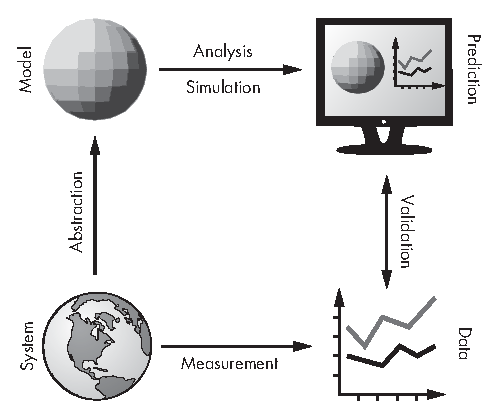
\includegraphics[scale=0.8]{images/figure01_01_new}}
  \index{modeling}
  \caption{The modeling process}
  \label{fig:modeling}
\end{figure}

\index{system}
\index{abstraction}


The result of abstraction is a \emph{model}, shown in the upper left; a model is a description of the system that includes only the features we think are essential.  A model can be represented in the form of diagrams and equations, which can be used for mathematical analysis.  It can also be implemented in the form of a computer program, which can run simulations.

\index{model}
\index{simulation}
\index{analysis}

The result of analysis and simulation might be a prediction about what the system will do, an explanation of why it behaves the way it does, or a specific design engineered to satisfy a requirement or optimize performance.

\index{prediction}
\index{explanation}
\index{design}

We can validate predictions and test designs by taking measurements from the real world and comparing the data we get with the results from analysis and simulation.

\index{validation}
\index{data}

For any physical system there are many possible models, each one including and excluding different features or including different levels of detail.  The goal of the modeling process is to find the model best suited to its purpose (prediction, explanation, or design).

\index{iterative modeling}

Sometimes the best model is the most detailed.  If we include more features, the model is more realistic, and we expect its predictions to be more accurate. \index{realism}
But often a simpler model is better.  If we include only the essential features and leave out the rest, we get models that are easier to work with, and the explanations they provide can be clearer and more compelling. \index{simplicity}

As an example, suppose someone asked you why the orbit of the Earth is nearly elliptical.  If you model the Earth and Sun as point masses (ignoring their actual size), compute the gravitational force between them using Newton's law of universal gravitation, and compute the resulting orbit  using Newton's laws of motion, you can show that the result is an ellipse.\index{orbit}\index{ellipse}

Of course, the actual orbit of Earth is not a perfect ellipse, because of the gravitational forces of the Moon, Jupiter, and other objects in the solar system, and because Newton's laws of motion are only approximately true (they don't take into account relativistic effects).
\index{Newton}%
\index{relativity}%

But adding these features to the model would not improve the explanation; more detail would only be a distraction from the fundamental cause.  However, if the goal is to predict the position of the Earth with great precision, including more details might be necessary.

Choosing the best model depends on what the model is for.  It is usually a good idea to start with a simple model, even if it's likely to be too simple, and test whether it's good enough for its purpose.  Then you can add features gradually, starting with the ones you expect to be most essential.  This process is called \emph{iterative modeling}.

\index{iterative modeling}

Comparing the results of successive models provides a form of \emph{internal  validation}, so you can catch conceptual, mathematical, and software errors.  And by adding and removing features, you can tell which ones have the biggest effect on the results, and which can be ignored.
\index{internal validation}%
\index{validation!internal}%
\index{external validation}%
\index{validation!external}%
Comparing results with data from the real world provides \emph{external validation}, which is generally the strongest test.

Figure~\ref{fig:modeling} shows that models can be used for both analysis and simulation; in this book we will do some analysis, but the focus is on simulation.  And the tool we will use to build simulations is MATLAB.  So let's get started.


\section{A Glorified Calculator}
\label{calc}

MATLAB is a programming language with features that support modeling and simulation.  It has a lot of features, so it can seem overwhelming, but at heart MATLAB is a glorified calculator.  When you start MATLAB you should see a window entitled MATLAB that contains smaller windows entitled Current Folder, Command Window, and Workspace.
%In Octave, Current Folder is called File Browser.

\index{Command Window}
\index{workspace}
\index{interpreter}
\index{command}

\subsection{The Interpreter}
The Command Window runs the \emph{interpreter}, which allows you
to enter \emph{commands}; once entered, the interpreter executes the command and prints the
result.
Initially, the Command Window contains a welcome message with information
about the version of the software you're running, followed by a \emph{prompt}, which looks like this:\index{prompt}

\begin{code}
>>
\end{code}

The \lstinline{>>} symbol prompts you to enter a command.
The simplest kind of command is a mathematical \emph{expression},
like \lstinline{2 + 1}.\index{expression}
If you type an expression and then press \keycap{enter} (or \keycap{return}), MATLAB
\emph{evaluates} the expression and prints the result.

\begin{code}
>> 2 + 1
ans = 3
\end{code}

Just to be clear: in this example, MATLAB displayed \lstinline{>>}; I
typed \textbf{\lstinline{2 + 1}} and then hit \keycap{enter}, and MATLAB displayed \lstinline{ans = 3}.

\index{operator}
\index{operand}

In this expression, the plus sign is an \emph{operator} and the numbers \lstinline{2} and \lstinline{1} are \emph{operands}.
An expression can contain any number of operators and operands.  You
don't have to put spaces between them; some people do and some people
don't. Here's an example with no spaces:

\begin{code}
>> 1+2+3+4+5+6+7+8+9
ans = 45
\end{code}

Speaking of spaces, you might have noticed that MATLAB puts a blank
line between \lstinline{ans =} and the result.  In my examples I'll leave it out to  save room.

\index{multiplication}
\index{division}
\index{arithmetic operator}
\index{exponentiation}

The other arithmetic operators are pretty much what you would expect.
Subtraction is denoted by a minus sign (\lstinline{-}), multiplication is designated by
an asterisk (\lstinline{*}), division is denoted by a forward slash (\lstinline{/}).

\begin{code}
>> 2*3 - 4/5
ans = 5.2000
\end{code}

Another common operator is exponentiation, which uses the \lstinline{^}
symbol, sometimes called ``caret'' or ``hat.''  So, 2 raised to the
16th power is

\begin{code}
>> 2^16
ans = 65536
\end{code}

The order of operations is what you would expect from basic algebra:
exponentiation happens before multiplication and division, and multiplication and division happen before addition and subtraction.
If you want to override the order of operations, you can use parentheses.

\index{operations!order of}
\index{order of operations}
\index{parentheses}

\begin{code}
>> 2 * (3-4) / 5
ans = -0.4000
\end{code}

When I added the parentheses, I removed some spaces to make the
grouping of operands clearer to a human reader.  This is the first
of many style guidelines I will recommend for making your programs
easier to read.  Style doesn't change what the program does; the MATLAB
interpreter doesn't check for style.  But human readers do, and the
most important human who will read your code is you.

\index{debugging!First Theorem}

And that brings us to the First Theorem of Debugging:

\begin{quote}
Readable code is debuggable code.
\end{quote}

It's worth spending time to make your code pretty; it will save
you time \mbox{debugging}!


\subsection{Math Functions}

MATLAB knows how to compute pretty much every math function you've
heard of. For example, it knows all the trigonometric functions---here's how you
use them:

\index{math function!trigonometric}

\begin{code}
>> sin(1)
ans = 0.8415
\end{code}

This command is an example of a \emph{function call}.  The name of the
function is \lstinline{sin}, which is the usual abbreviation for the
trigonometric sine.  The value in parentheses is called the \emph{argument}.
\index{argument}%
\index{function!argument}%

The trig functions \lstinline{sin}, \lstinline{cos}, and  \lstinline{tan}---among many
others---work in radians, so the argument in the example is interpreted as 1~radian.
MATLAB also provides trig functions that work in degrees: \lstinline{sind}, \lstinline{cosd}, and \lstinline{tand}.

Some functions take more than one argument, in which case the arguments are
separated by commas.  For example, \lstinline{atan2} computes the inverse
tangent, which is the angle in radians between the positive x-axis and
the point with the given x- and y-coordinates.

\begin{code}
>> atan2(1,1)
ans = 0.7854
\end{code}

If that bit of trigonometry isn't familiar to you, don't worry about
it.  It's just an example of a function with multiple arguments.

\index{trigonometry}
\index{math function!exponential}

MATLAB also provides exponential functions, like \lstinline{exp}, which computes $e$ raised to the given power.  So \lstinline{exp(1)} is just $e$:

\begin{code}
>> exp(1)
ans = 2.7183
\end{code}

\index{math function!logarithm}

The inverse of \lstinline{exp} is \lstinline{log}, which computes the logarithm base $e$:

\begin{code}
>> log(exp(3))
ans = 3
\end{code}

This example also demonstrates that function calls can be \emph{nested};
that is, you can use the result from one function as an argument for
another.

\index{nested function call}
\index{function call!nested}
\index{operand}

More generally, you can use a function call as an operand in an \mbox{expression}.

\begin{code}
>> sqrt(sin(0.5)^2 + cos(0.5)^2)
ans = 1
\end{code}

As you probably guessed, \lstinline{sqrt} computes the square root.

\index{math function!square root}

There are lots of other math functions, but this isn't meant to
be a reference manual.  To learn about other functions, you should
read the documentation.


\section{Variables}

Of course, MATLAB is good for more than just evaluating expressions. One of the features that makes MATLAB more powerful than a calculator is the ability to give a name to a value.  A named value is called a \emph{variable}.

\index{variable}
\index{variable!predefined}
\index{predefined variable}

MATLAB comes with a few predefined variables. For
example, the name \lstinline{pi} refers to the
mathematical quantity $\pi$, which is approximately this:

\begin{code}
>> pi
ans = 3.1416
\end{code}

And if you do anything with complex numbers, you might find it
convenient that both \lstinline{i} and \lstinline{j} are predefined as the square
root of $-1$.

\index{complex number!imaginary unit}
\index{operand}
\index{expression}

You can use a variable name anywhere you can use a number---for example, as
an operand in an expression,

\begin{code}
>> pi * 3^2
ans = 28.2743
\end{code}
or as an argument to a function:

\begin{code}
>> sin(pi/2)
ans = 1
\end{code}

\index{argument}
\index{function call}

Whenever you evaluate an expression, MATLAB assigns the result to
a variable named \lstinline{ans}.  You can use \lstinline{ans} in a subsequent
calculation as shorthand for ``the value of the previous expression.''

\begin{code}
>> 3^2 + 4^2
ans = 25

>> sqrt(ans)
ans = 5
\end{code}

But keep in mind that the value of \lstinline{ans} changes every time
you evaluate an expression.


\subsection{Assignment Statements}

You can create your own variables, and give them values, with
an \emph{assignment statement}.  The assignment operator is the
equals sign (\lstinline{=}), used like so:

\index{assignment operator}
\index{operator!assignment}
\index{statement!assignment}

\begin{code}
>> x = 6 * 7
x = 42
\end{code}

This example creates a new variable named \lstinline{x} and assigns it the
value of the expression \lstinline{6 * 7}.  MATLAB responds with the
variable name and the computed value.

\index{expression}

There are a few rules when assigning variables a value. In every assignment statement, the left side has to be a legal variable name.  The right side can be any expression, including function calls.
\index{variable!name}%
\index{name!variable}%
\index{underscore}%
\index{case sensitive}%
Almost any sequence of lower- and uppercase letters is a legal
variable name.
Some punctuation is also legal, but the underscore (\lstinline{_}) is the only commonly used non-letter.
Numbers are fine, but not at the beginning.
Spaces are not allowed.  Variable names are
\emph{case-sensitive}, so \lstinline{x} and \lstinline{X} are different variables.

Let's look at some examples of assignment statements.

\begin{code}
>> fibonacci0 = 1;

>> LENGTH = 10;

>> first_name = 'bob'
first_name = 'bob'
\end{code}

The first two examples demonstrate the use of the semicolon, which
suppresses the output from a command.  In this case MATLAB creates the
variables and assigns them values but displays nothing.
\index{syntax!semicolon}%
\index{semicolon}%
\index{suppress output}%
\index{output!suppress}%

The third example demonstrates that not everything
in MATLAB is a number.
A sequence of characters in single quotes is
a \emph{string}.

\index{string}
\index{character}

Although \lstinline{i}, \lstinline{j}, and \lstinline{pi} are predefined, you are free
to reassign them.  It's common to use \lstinline{i} and \lstinline{j} for other
purposes, but it's rare to assign a different value to
\lstinline{pi}.

\index{complex number!imaginary unit}


\subsection{Variables in the Workspace}

When you create a new variable, it appears in the Workspace window and is added to the \emph{workspace}, which is a
set of variables and their values.

\index{variable}
\index{workspace}

The \lstinline{who} command prints the
names of the variables in the workspace:

\index{who@\lstinline{who}}
% \index{command!\lstinline{who}}

\begin{code}
>> x = 5;
>> y = 7;
>> z = 9;
>> who

Your variables are:

x  y  z
\end{code}

This information, what variables are in the current workspace, is also shown in the "Workspace" widget in the MATLAB integrated development environment (IDE).  The default layout has this widget on the right side of the MATLAB IDE window.

The \lstinline{clear} command removes specified variables from the workspace:

\begin{code}
>> clear x
>> who

Your variables are:

y z
\end{code}

But be careful: if you don't specify any variables, \lstinline{clear} removes them all.

\index{clear@\lstinline{clear}}
\index{disp@\lstinline{disp}}

To display the value of a variable, you can use the \lstinline{disp} function:

\begin{code}
>> disp(z)
     9
\end{code}
but it's easier to just type the variable name:

\begin{code}
>> z
z = 9
\end{code}

Now that you've seen how to use them, let's take a step back and think about why we'd use variables.

\subsection{Why Variables?}

There are a number of reasons to use variables.\index{variable!reasons for}
A big one is to avoid recomputing a value you use repeatedly.  For
example, if your computation uses $e$ frequently, you might
want to compute it once and save the result.

\begin{code}
>> e = exp(1)
e = 2.7183
\end{code}

Variables also make the connection between the code and the underlying
mathematics more apparent.  If you're computing the area of a circle,
you might want to use a variable named \lstinline{r}:

\begin{code}
>> r = 3
r = 3

>> area = pi * r^2
area = 28.2743
\end{code}

That way, your code resembles the familiar formula $a = \pi r^2$.

You might also use a variable to break a long computation into a sequence of steps.
Suppose you're evaluating a big, hairy expression like this:

\begin{code}
p = ((x - theta) * sqrt(2 * pi) * sigma)^-1 * ...
exp(-1/2 * (log(x - theta) - zeta)^2 / sigma^2)
\end{code}

You can use an ellipsis to break the expression into multiple lines.
Just enter \lstinline{...} at the end of the first line and continue on to the
next.
\index{syntax!\lstinline{...}}
\index{ellipsis}But often it's better to break the computation into a sequence of
steps and assign intermediate results to variables:

\begin{code}
shiftx = x - theta
denom = shiftx * sqrt(2 * pi) * sigma
temp = (log(shiftx) - zeta) / sigma
exponent = -1/2 * temp^2
p = exp(exponent) / denom
\end{code}

The names of the intermediate variables explain their role in the
computation:  \lstinline{shiftx} is the value of \lstinline{x} shifted by
\lstinline{theta},  it should be no surprise that \lstinline{exponent} is the argument of \lstinline{exp}, and \lstinline{denom} ends up in the denominator.  Choosing informative names makes the code easier to read and understand, which makes it easier to debug.

\index{numerator}
\index{denominator}


\section{Errors}

\index{error}

Every error is a learning opportunity.
Whenever you learn a new feature, you should try to make as many errors as possible, as soon as possible.
When you make deliberate errors, you see what the error messages are.
Later, when you make accidental errors, you'll know what the messages mean.

Let's look at some common errors. A big one for beginners is leaving out the \lstinline{*}
for multiplication, as in this example:

\begin{code}
area = pi r^2
\end{code}

This code should produce the following error message:

\begin{stdout}
 area = pi r^2
           |
Error: Invalid expression. Check for missing multiplication
operator, missing or unbalanced delimiters, or other syntax
error. To construct matrices, use brackets instead of parentheses.
\end{stdout}
\index{invalid expression}%
\index{expression!invalid}%

The message indicates that the expression is invalid and suggests several things that might be wrong.
In this case, one of its guesses is right: we're missing a multiplication operator.

\index{parentheses}

Another common error is to leave out the parentheses around the
arguments of a function.  For example, in math notation it's common
to write something like $\sin \pi$, but in MATLAB if you write

\begin{code}
sin pi
\end{code}
you should get the following error message:

\begin{stdout}
Undefined function 'sin' for input arguments of type 'char'.
\end{stdout}

The problem is that when you leave out the parentheses, MATLAB treats
the argument as a string of characters (which have type \lstinline{'char'}).
In this case the error message is helpful, but in other cases the results can be baffling.
For example, if you call \lstinline{abs}, which computes absolute values, and forget the parentheses, you get a surprising result:

\begin{code}
>> abs pi
ans =  112   105
\end{code}

I won't explain this result; for now, I'll just suggest that you should \mbox{\emph{always}} put parentheses around arguments.

\index{error message}

Here's another common error.
If you were translating the mathematical expression
%
\[ \frac{1}{2 \sqrt \pi} \]
%
into MATLAB, you might be tempted to write this:

\begin{code}
1 / 2 * sqrt(pi)
\end{code}

But that would be wrong because of the order of operations.  Division and multiplication are evaluated from left to right, so this expression would multiply \lstinline{1/2} by \lstinline{sqrt(pi)}.

\index{order of operations}
\index{denominator}

To keep \lstinline{sqrt(pi)} in the denominator, you could use parentheses,

\begin{code}
1 / (2 * sqrt(pi))
\end{code}
or make the division explicit,

\begin{code}
1 / 2 / sqrt(pi)
\end{code}

\index{division}
\index{debugging!Second Theorem}

The last two examples bring us to the Second Theorem of Debugging:

\begin{quote}
The only thing worse than getting an error message is \emph{not} getting an error message.
\end{quote}

Beginning programmers often hate error messages and do everything they
can to make the messages go away.  Experienced programmers know that error
messages are your friend.  They can be hard to understand, and even
misleading, but it's worth the effort to understand them.

\section{Documentation}

MATLAB comes with two forms of documentation, \lstinline{help}
and \lstinline{doc}.
\index{documentation!doc@\lstinline{doc}}
\index{documentation!help@\lstinline{help}}The \lstinline{help} command works in the Command Window; just
enter \textbf{\lstinline{help}} followed by the name of a command.

% Here's an example where the output is in a stdout environment to
% avoid nonsensical syntax highlighting.

\begin{code}
>> help sin
\end{code}

You should see output like this:

\begin{stdout}
 sin    Sine of argument in radians.
    sin(X) is the sine of the elements of X.

    See also asin, sind, sinpi.
\end{stdout}

Some documentation uses vocabulary we haven't covered yet.
For example, \lstinline{the elements of X} might not make sense until
we get to vectors and matrices a few chapters from now.

\index{element}
\index{vector}
\index{matrix}

The \lstinline{doc} pages are usually better.  You can access the \lstinline{doc} pages in at least two ways:

\begin{enumerate}
\item If you enter \lstinline{doc sin}, a browser window appears with more detailed information about the function, including examples of how to use it. 
\item If you do a web search for "matlab sin" you will find the same documentation in one of the first results.
\end{enumerate}
The examples often use vectors and matrices, so they may not make sense yet,
but you can get a preview of what's coming.


\section{Chapter Review}

This chapter provided an overview of the modeling process, including abstraction, analysis and simulation, measurement, and validation.

It also introduced MATLAB, the programming language we'll use to write simulations.  So far, we've seen variables and values, arithmetic operations, and mathematical functions.

Here are a few terms from this chapter you might want to remember.

The \emph{interpreter} is the program that reads and executes MATLAB or \mbox{Octave} code.
It prints a \emph{prompt} to indicate that it's waiting for you to type a \emph{command}, which is a line of code executed by the interpreter.

An \emph{operator} is a symbol, like \lstinline{*} or \lstinline{+}, that
represents a mathematical operation.
An \emph{operand} is a number or variable that appears in an expression along
with operators.
An \emph{expression} is a sequence of operands and operators that specifies
a mathematical computation and yields a value.

A \emph{function} is a named computation; for example, \lstinline{log10} is the
name of a function that computes logarithms in base 10.
A \emph{function call} is a command that causes a function to execute and compute a result.
An \emph{argument} is an expression that appears in a function call to
specify the value the function operates on.

A \emph{variable} is a named value. An \emph{assignment statement} is a command that creates a new variable (if necessary) and gives it a value.
A \emph{workspace} is a set of variables and their values.

Finally, a \emph{string} is a value that consists of a sequence of characters (as opposed to a number).

In the next chapter, you'll start writing longer programs and learn about floating-point numbers.

\section{Exercises}

Before you go on, you might want to work on the following exercises.

\begin{ex}
\label{penny}
You might have heard that a penny dropped from the top of the Empire State Building would be going so fast when it hit the pavement that it would be embedded in the concrete or that if it hit a person it would break their skull.

\index{Empire State Building}
\index{penny}
\index{myth}

We can test this myth by making and analyzing a model.  To get started, we'll assume that the effect of air resistance is small.  This will turn out to be a bad assumption, but bear with me.

If air resistance is negligible, the primary force acting on the penny is gravity, which causes the penny to accelerate downward.

\index{air resistance}

If the initial velocity is 0, the velocity after $t$ seconds is $a t$, and the distance the penny has dropped is
%
\[ h = a t^2 / 2 \]
%
Using algebra, we can solve for $t$:
%
\[ t = \sqrt{ 2 h / a} \]
%
Plugging in the acceleration of gravity,
$a = \SI{9.8}{\meter\per\second\squared}$, and the height of the Empire State Building,
$h = \SI{381}{\meter}$, we get
$t = \SI{8.8}{\second}$.
Then, computing $v = a t$ we get a velocity on impact of $\SI{86}{\meter\per\second}$, which is about 190 miles per hour.  That sounds like it could hurt.

Use MATLAB to perform these computations, and check that you get the same result.
\end{ex}

\begin{ex}
The result in the previous exercise is not accurate because it ignores air resistance.  In reality, once the penny gets to about \SI{18}{\meter\per\second}, the upward force of air resistance equals the downward force of gravity, so the penny stops accelerating.  After that, it doesn't matter how far the penny falls; it hits the sidewalk at about \SI{18}{\meter\per\second}, much less than \SI{86}{\meter\per\second}.

As an exercise, compute the time it takes for the penny to reach the sidewalk if we assume that it accelerates with constant acceleration
$a = \SI{9.8}{\meter\per\second\squared}$ until it reaches terminal velocity, then falls with constant velocity until it hits the sidewalk.

The result you get is not exact, but it's a pretty good approximation.
\end{ex}

\chapter{Scripts and Live Scripts}

So far we've typed all of our programs ``at the prompt.'' If you're only writing a few lines, this isn't so bad. But what if you're writing a hundred? Retyping each line of code every time you want to change or test your program will be time-consuming and tedious. Luckily, you don't have to. In this chapter, we'll look at two ways to run many lines at once: \emph{scripts} and \emph{live scripts}.

But, before we get to that let's discuss the generic term - a program.

\section[What is a program?]{What is a program?\protect\footnote{This section is from Allen Downey's book, \href{https://greenteapress.com/wp/think-python-2e/}{Think Python}, 2e Edition.}}

A {\bf program} is a sequence of instructions that specifies how to
perform a computation.  The computation might be something
mathematical, such as solving a system of equations or finding the
roots of a polynomial, but it can also be a symbolic computation, such
as searching and replacing text in a document or something
graphical, like processing an image or playing a video.
\index{program}

The details look different in different languages, but a few basic
instructions appear in just about every language:

\begin{description}

\item[input:] Get data from the keyboard, a file, the network, or some
other device.

\item[output:] Display data on the screen, save it in a
file, send it over the network, etc.

\item[math:] Perform basic mathematical operations like addition and
multiplication.

\item[conditional execution:] Check for certain conditions and
run the appropriate code.

\item[repetition:] Perform some action repeatedly, usually with
some variation.

\end{description}

Believe it or not, that's pretty much all there is to it.  Every
program you've ever used, no matter how complicated, is made up of
instructions that look pretty much like these.  So you can think of
programming as the process of breaking a large, complex task
into smaller and smaller subtasks until the subtasks are
simple enough to be performed with one of these basic instructions.

\section{Scripts}

A \emph{script} is a file that contains a MATLAB program. When you run a script, MATLAB executes the commands in it, one after another, exactly as if you had typed them at the prompt. Scripts are
also sometimes called \emph{M-files} because they use the extension \emph{.m}, short for MATLAB.

\index{script}
\index{M-file}
\index{file extension}

\subsection{Your First Script}

You can create scripts with any text editor or word processor, but the simplest way is to click the \textbf{New->Script} button in the upper-left corner of the MATLAB interface, which opens a text editor designed for MATLAB, simpl;y called the "Editor".

To try it out, create a new script and enter the following code:

\begin{code}
x = 5
\end{code}

Then press the \textbf{Save} button.  A dialog window should appear where you can choose the filename and the folder where your script will go.
Change the name to \emph{myscript.m} and save it into any folder you like.

Now click the green \textbf{Run} button.  You might get a message that says the script is not found in the current folder.
If so, click the button that says Change Folder and it should run.  

A handy way to discover the current folder in which the Command Window is operating is to issue the \lstinline{pwd} command - for 'print working directory'.  You can also issue the \lstinline{ls} command to display a listing of the files and folders in the current working directory, for example
\begin{code}
  >> ls
bike_update.m	     fibonacci1_live.pdf  mylivescript.mlx  myscript.m
fibonacci1_live.mlx  fibonacci1.m	  mylivescript.pdf  swap.m
\end{code}

\index{Command Window}

\textbf{Pro Tip:} You will likely find you run scripts, or portions of a script, frequently while you are developing, testing and debugging.  The keyboard shorcuts can speed up this interation cycle.  To run the entire script the \textbf{F5} key is equivalent to clicking the Run button and to typing the name of the script in the Command Window.  To run just a portion of your script, highlight that section and press the \textbf{Ctrl+Enter} keys.

You can also run a script by typing its name in the Command Window and pressing \keycap{enter}. For example, if you enter \lstinline{myscript}, MATLAB should execute your script and display the result:

\begin{code}
>> myscript
x = 5
\end{code}

There are a few things to keep in mind when using scripts. First, you should not include the extension \emph{.m} when you run a script.  If you do, you'll get an error message like this:

\begin{code}
>> myscript.m
Undefined variable "myscript" or class "myscript.m".
\end{code}

Second, when you name a new script, try to choose something meaningful and memorable.
Don't choose a name that's already in use; if you do, you'll replace one of MATLAB's functions with your own (at least temporarily).
You might not notice right away, but you might get some confusing behavior later.

\index{script!filename}

Also, the name of the script cannot contain spaces.  If you create
a file named \emph{my script.m}, MATLAB will complain when you try
to run it:

\begin{code}
>> my script
Undefined function or variable 'my'.
\end{code}

It can be hard to remember which folder a script is in.  To keep things simple,
for now, I suggest putting all of your scripts in one folder.

\subsection{Why Scripts?}

There are a few good reasons to use a script. When you're writing more than a couple of lines of code, it might take a few tries to get everything right.  Putting your code
in a script makes it easier to edit than typing it at the prompt. Likewise, if you're running a script repeatedly, it's much faster to type the name of the script than to retype the code! And you might be able to reuse a script from one project to the next, saving you considerable time across projects.

\index{script!reasons for}


But the great power of scripts comes with great responsibility: you have to make sure that the code you are running is the code you think you are running.
Whenever you start a new script, start with something simple, like \lstinline{x = 5}, that produces a visible effect. Then run your script and confirm that you get what you expect.
When you type the name of a script, MATLAB searches for the script in a \emph{search path}, which is a sequence of folders.  If it doesn't find the script in the first folder, it searches the second, and so on.
If you have scripts with the same name in different folders, you could be looking at one version and running another.

\index{search path}
\index{folder}

\index{debugging!Third Theorem}

If the code you are running is not the code you are looking
at, you'll find debugging a frustrating exercise!  So it's no surprise that this is the Third Theorem of Debugging:

\begin{quote}
Be sure that the code you are running
is the code you think you are running.
\end{quote}

Now that you've seen how to write a script, let's use one to do something a little more complicated.

\subsection{Example: The Fibonacci Sequence}

\index{Fibonacci number}
\index{sequence!Fibonacci}

The \emph{Fibonacci sequence}, denoted $F$, is a sequence of numbers where each number is the sum of the previous two.
It's defined by the equations $F_1 = 1$, $F_2 = 1$, and, for $i > 2$, $F_{i} = F_{i-1} + F_{i-2}$.
The following expression computes the $n$th Fibonacci number:
%
\begin{equation*}
F_n = \frac{1}{\sqrt{5}}
\left[
\left( \frac{1 + \sqrt{5}}{2} \right)^{n} -
\left( \frac{1 - \sqrt{5}}{2} \right)^{n}
\right]
\end{equation*}
%

We can translate this expression into MATLAB, like this:

\begin{code}
s5 = sqrt(5);
t1 = (1 + s5) / 2;
t2 = (1 - s5) / 2;
diff = t1^n - t2^n;
ans = diff / s5
\end{code}

I use temporary variables like \lstinline{t1} and \lstinline{t2} to make the code readable and the order of operations explicit.  The first four lines have a semicolon at the end, so they don't display anything.  The last line assigns the result to \lstinline{ans}.

\index{semicolon}

If we save this script in a file named \emph{fibonacci1.m}, we can run it like this:

\begin{code}
>> n = 10
>> fibonacci1
ans = 55.0000
\end{code}

Before calling this script, you have to assign a value to \lstinline{n}.
If \lstinline{n} is not defined, you get an error:

\begin{code}
>> clear n
>> fibonacci1
Undefined function or variable 'n'.

Error in fibonacci1 (line 9)
diff = t1^n - t2^n;
\end{code}

This script only works if there is a variable named \lstinline{n} in the workspace; otherwise, you should get an error.
MATLAB will tell you what line of the script the error is in and display the line.

\index{workspace}

\index{debugging!Fourth Theorem}

Error messages can be helpful, but beware!
In this example, the message says the error is in \lstinline{fibonacci}, but the actual problem is that we have not assigned a value to \lstinline{n}.
And that brings us to the Fourth Theorem of Debugging:

\begin{quote}
Error messages tell you where the problem was discovered,
not where it was caused.
\end{quote}

Often you have to work backwards to find the line of code (or missing line) that caused the problem.

\subsection{Floating-Point Numbers}

In the previous section, the result we computed was \lstinline{55.0000}.  Since the Fibonacci numbers are integers, you might have been surprised to see the zeros after the decimal point.

They are there because MATLAB performs calculations using floating-point numbers.  With \emph{floating-point numbers}, integers can be represented exactly, but most fractions cannot.

\index{floating-point}
\index{number!floating-point}

For example, if you compute the fraction 2/3, the result is only approximate---the correct answer has an infinite number of 6s:

\begin{code}
>> 2/3
ans = 0.6666
\end{code}



It's not as bad as this example makes it seem: MATLAB uses more digits than it shows by default.
You can use the \lstinline{format} command to change the output format:

\index{format@\lstinline{format}}

\begin{code}
>> format long
>> 2/3
ans = 0.666666666666667
\end{code}

In this example, the first 14 digits are correct; the last one has been rounded off.

\index{scientific notation}
\index{factorial@\lstinline{factorial}}

Large and small numbers are displayed in \emph{scientific notation}.
For example, if we use the built-in function \lstinline{factorial} to compute $100!$, we get the following result:

\begin{code}
>> factorial(100)
ans = 9.332621544394410e+157
\end{code}

The \lstinline{e} in this notation is \emph{not} the transcendental number
known as $e$; it's just an abbreviation for ``exponent.''  So
this means that $100!$ is approximately $9.33 \times 10^{157}$.  The
exact solution is a 158-digit integer, but with double-precision floating-point numbers, we only know the first 16 digits.

\index{transcendental number}
\index{exponent}

You can enter numbers using the same notation.

\begin{code}
>> speed_of_light = 3.0e8
speed_of_light = 300000000
\end{code}

Although the floating-point format can represent very large and small numbers,
there are limits.
The predefined variables \lstinline{realmax} and \lstinline{realmin}
contain the largest and smallest numbers MATLAB
can handle.

\index{realmin@\lstinline{realmin}}
\index{realmax@\lstinline{realmax}}

\begin{code}
>> realmax
ans = 1.797693134862316e+308

>> realmin
ans = 2.225073858507201e-308
\end{code}

If the result of a computation is too big, MATLAB ``rounds up''
to \mbox{infinity}.

\index{Inf@\lstinline{Inf}}

\begin{code}
>> factorial(170)
ans = 7.257415615307994e+306

>> factorial(171)
ans = Inf
\end{code}

Division by zero also returns \lstinline{Inf}.

\begin{code}
>> 1/0
ans = Inf
\end{code}

\index{division!by zero}
\index{zero!division by}

For operations that are undefined, MATLAB returns \lstinline{NaN},
which stands for ``not a number.''

\index{NaN@\lstinline{NaN}}
\index{not a number}
\index{undefined operation}

\begin{code}
>> 0/0
ans = NaN
\end{code}


\subsection{Comments}

Short, simple programs are easy to read, but as they get bigger and more complex, it gets harder to figure out what they do and how.  That's what comments are for.

A \emph{comment} is a line of text added to a program to explain how it works. It has no effect on the execution of the program; it is there for human readers.
Good comments make programs more readable; bad comments are useless at best and misleading at worst.

To write a comment, you use the percent symbol (\%) followed by the text of the comment.

\index{comment}
\index{\%@\lstinline{\%}}
\index{percent sign}

\begin{code}
>> speed_of_light = 3.0e8     % meters per second
speed_of_light = 300000000
\end{code}

The comment runs from the percent symbol to the end of the line.
In this case it specifies the units of the value.  In an ideal world,
MATLAB would keep track of units and propagate them through the
computation, but for now that burden falls on the programmer.

\index{unit}

Avoid comments that are redundant with the code:

\begin{code}
>> x = 5        % assign the value 5 to x
\end{code}

Good comments provide additional information that's not in the
code, like units in the example above, or the meaning of a variable:

\begin{code}
>> p = 0         % position from the origin in meters
>> v = 100       % velocity in meters / second
>> a = -9.8      % acceleration of gravity in meters / second^2
\end{code}

If you use longer variable names, you might not need explanatory
comments, but there's a trade-off: longer variable names are clearer, but longer code can become harder
to read.
Also, if you're translating from math
that uses short variable names, it can be useful to make your
program consistent with your math.

\index{variable name}

\subsection{Documentation}

Every script should provide \emph{documentation}, which is a comment
that explains what the script does and what its requirements are.

For example, I might put something like this at the beginning of \emph{fibonacci1.m}:

\index{documentation!function}
\index{function!documentation}

\begin{code}
% Computes a numerical approximation of the nth Fibonacci number.
% Precondition: you must assign a value to n before running this script.
% Postcondition: the result is stored in ans.
\end{code}

A \emph{precondition} is something that must be true when the script
starts in order for it to work correctly.  A \emph{postcondition}
is something that will be true when the script completes.

\index{precondition}
\index{postcondition}
\index{Fibonacci}

If there is a comment at the beginning of a script, MATLAB assumes
it's the documentation for the script. So if you type \lstinline{help fibonacci1}, you get the contents of the comment (without the percent
signs).

\begin{code}
>> help fibonacci1
  Computes a numerical approximation of the nth Fibonacci number.
  Precondition: you must assign a value to n before running this script.
  Postcondition: the result is stored in ans.
\end{code}

That way, scripts that you write behave just like predefined scripts.
You can even use the \lstinline{doc} command to see your comment in the
Help Window.

\index{Help Window}
\index{doc@\lstinline{doc}}
\index{help@\lstinline{help}}

\subsection{Assignment and Equality}

For beginning programmers, a common source of confusion is assignment and the use of the equals sign.

\index{variable!assignment}
\index{assignment!target}
\index{equality}

In mathematics, the equals sign means that the two sides of the
equation have the same value.
In MATLAB, an assignment statement \emph{looks} like a mathematical equality, but it's not.

One difference is that the sides of an assignment statement are not
interchangeable.  The right side can be any legal expression, but
the left side has to be a variable, which is called the
\emph{target} of the assignment.  So this is legal:

\begin{code}
>> y = 1;
>> x = y + 1
x = 2
\end{code}

But this is not:

\begin{code}
>> y + 1 = x
 y + 1 = x
       |
Error: Incorrect use of '=' operator.
To assign a value to a variable, use '='.
To compare values for equality, use '=='.
\end{code}

In this case the error message is not very helpful.  The problem here is that the expression on the left side is not a valid target for an assignment.

\index{error message}

Another difference between assignment and equality is that a mathematical equality is true (or false) for all eternity;
an assignment statement is temporary.
When you assign \lstinline{x = y + 1}, you get the
\emph{current} value of \lstinline{y}.  If \lstinline{y} changes later, \lstinline{x}
does not get updated.

A third difference is that a mathematical equality is a statement that
may or may not be true.  In mathematics, $y = y+1$ is a statement that
happens to be false for all values of $y$.
In MATLAB, \lstinline{y = y + 1} is a sensible and useful assignment statement.
It reads the current value of \lstinline{y}, adds 1, and replaces the old value with the new value.

\begin{code}
>> y = 1;
>> y = y + 1
y = 2
\end{code}

When you read MATLAB code, you might find it helpful to pronounce
the equals sign as ``gets'' rather than ``equals.''  So \lstinline{x = y + 1}
is pronounced ``\lstinline{x}~gets the value of \lstinline{y} plus one.''

\section{Live Scripts}

A MATLAB \emph{live script} is an interactive document that combines code, formatted text (e.g., equations), images and output in once place.  In one sense it merges the code from a script with the execution of the command window.  A live script allows you to run sections of your program independently, debugging as you go, while embedding the computation in a portable document that you can export and share.

\subsection{Your First Live Script}

While regular (non-live) scripts are stored as a text file with the \emph{.m} extension, live scripts are stored as package of code, rich text and images.   Luckily, MATLAB hides all this complexity from the user and what you see is a single document, stored as a \emph{.mlx} file.

You can create a live script by clicking the \textbf{New->Live Script} button in the upper-left corner of the MATLAB interface.  This opens the MATLAB "Live Editor".  Create a new live script and add the following:

\begin{enumerate}
\item Add a text block.  This is rich text that can be formatted using the buttons on the top of the Live Editor or using \href{https://www.mathworks.com/help/matlab/matlab_prog/format-live-scripts.html}{markdown}.
\item Add a code block with the line \lstinline{x = 5}.
\end{enumerate}

Then press the \textbf{Save} button to save the file as \emph{mylivescript.mlx}.

Now click the same green \textbf{Run} button (or hit F5) to run the script and see the result in the same document.  You can still call the live script from the Command Window:
\begin{code}
  >> mylivescript
  x =
       5
\end{code}
But that is probably a rare use-case.

In addition to saving the live script as an \emph{.mlx} file, you can also export the document in a variety of formats.  Here is what the PDF export might look like:


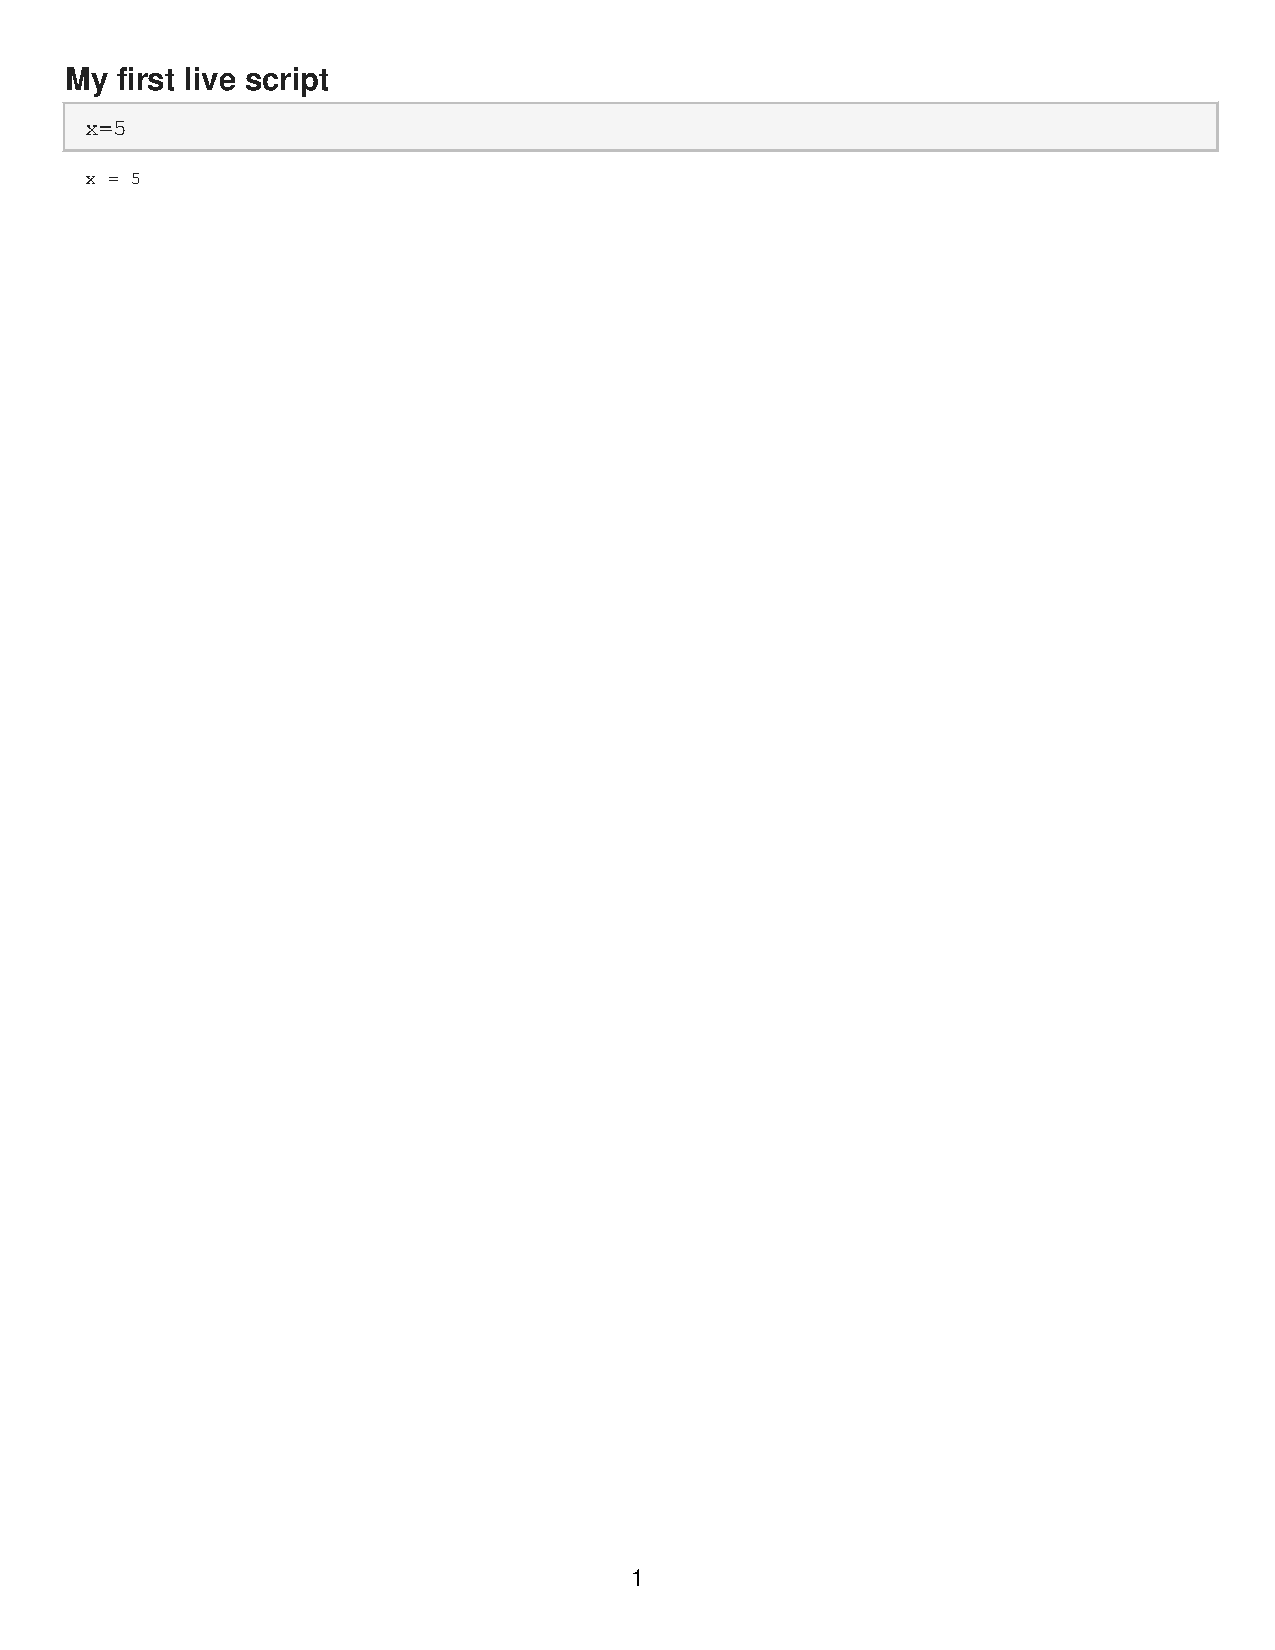
\includepdf[pages=-,frame,pagecommand={},width=0.9\textwidth]{w03_modeling_scripts/lessons/mylivescript.pdf}

\subsection{Example: The Fibonacci Sequence}

Returning to our earlier example of a plain script, we can now combine the rich text of the description, including the expression for the Fibonacci number, into a live script with alternating text and code blocks.  The resulting PDF would look something like this: 

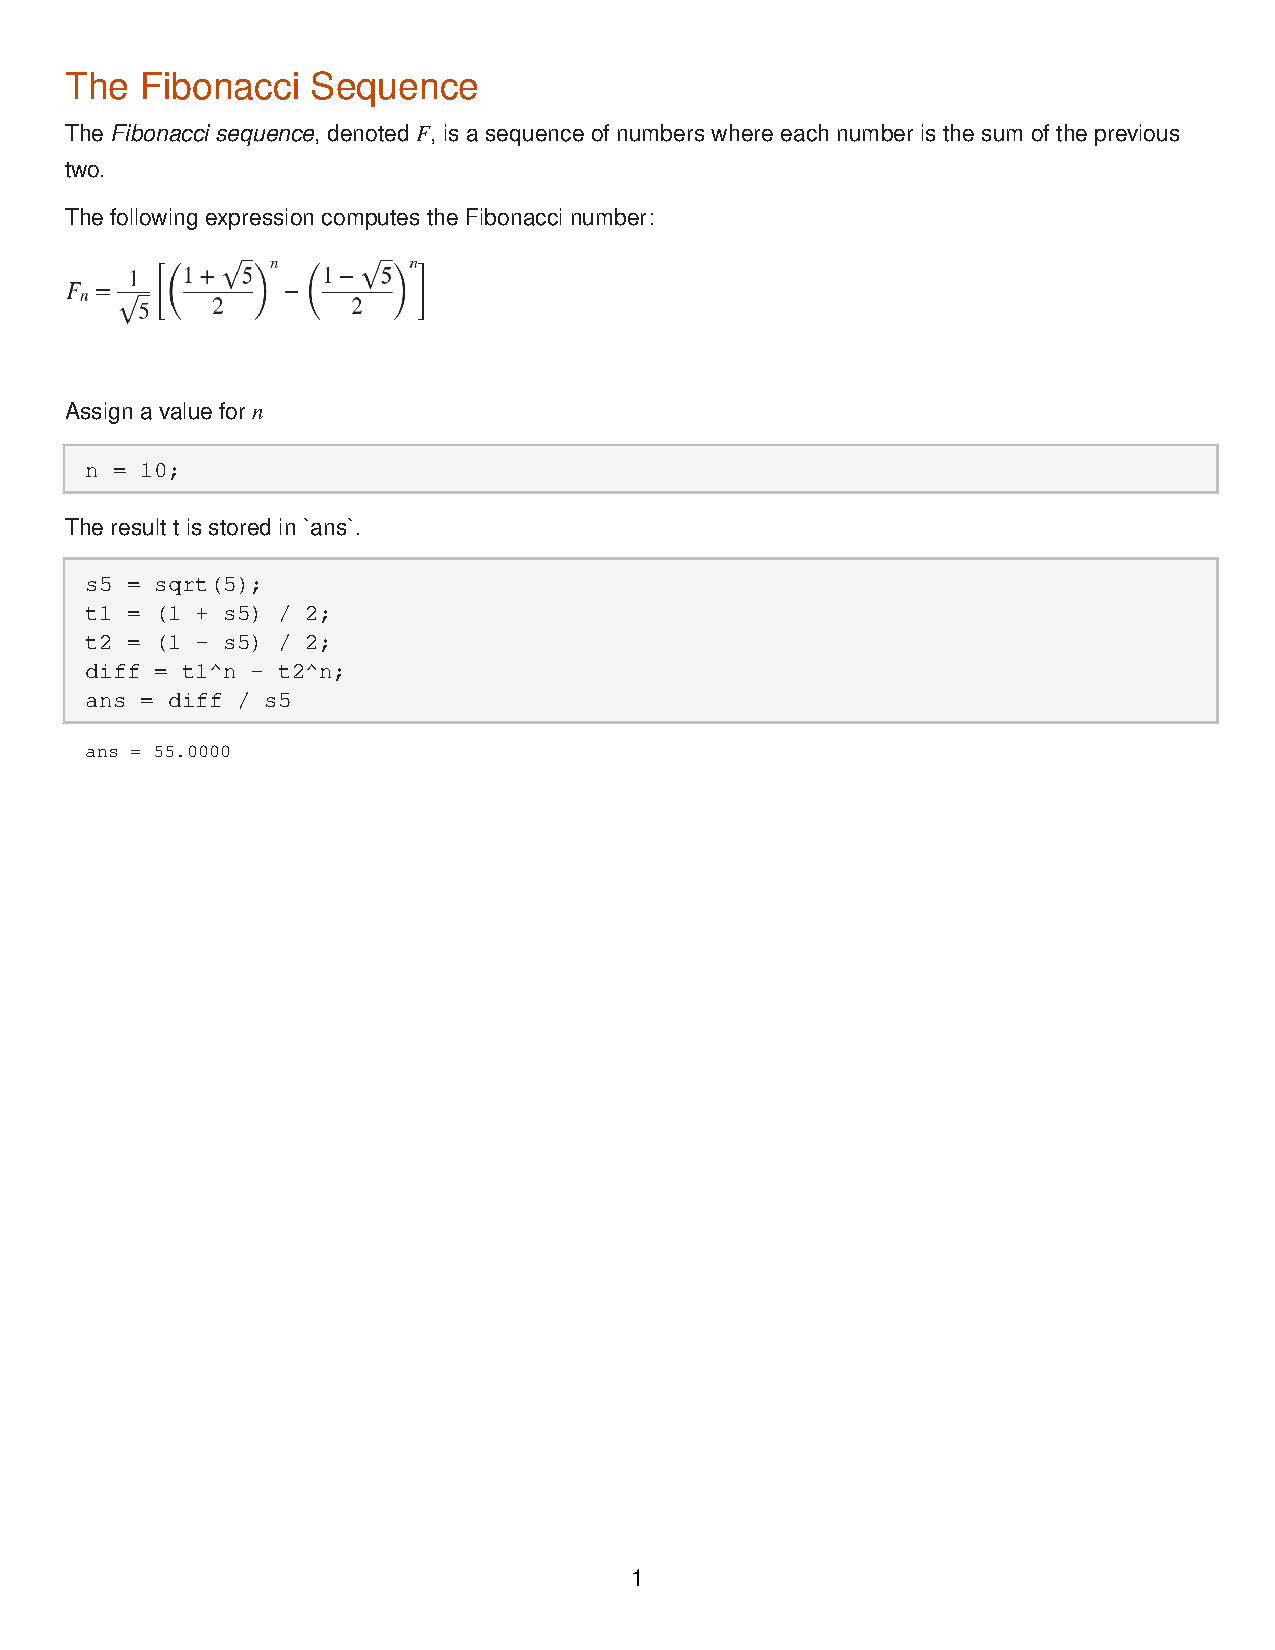
\includepdf[pages=-,frame,pagecommand={},width=0.9\textwidth]{w03_modeling_scripts/lessons/fibonacci1_live.pdf}
%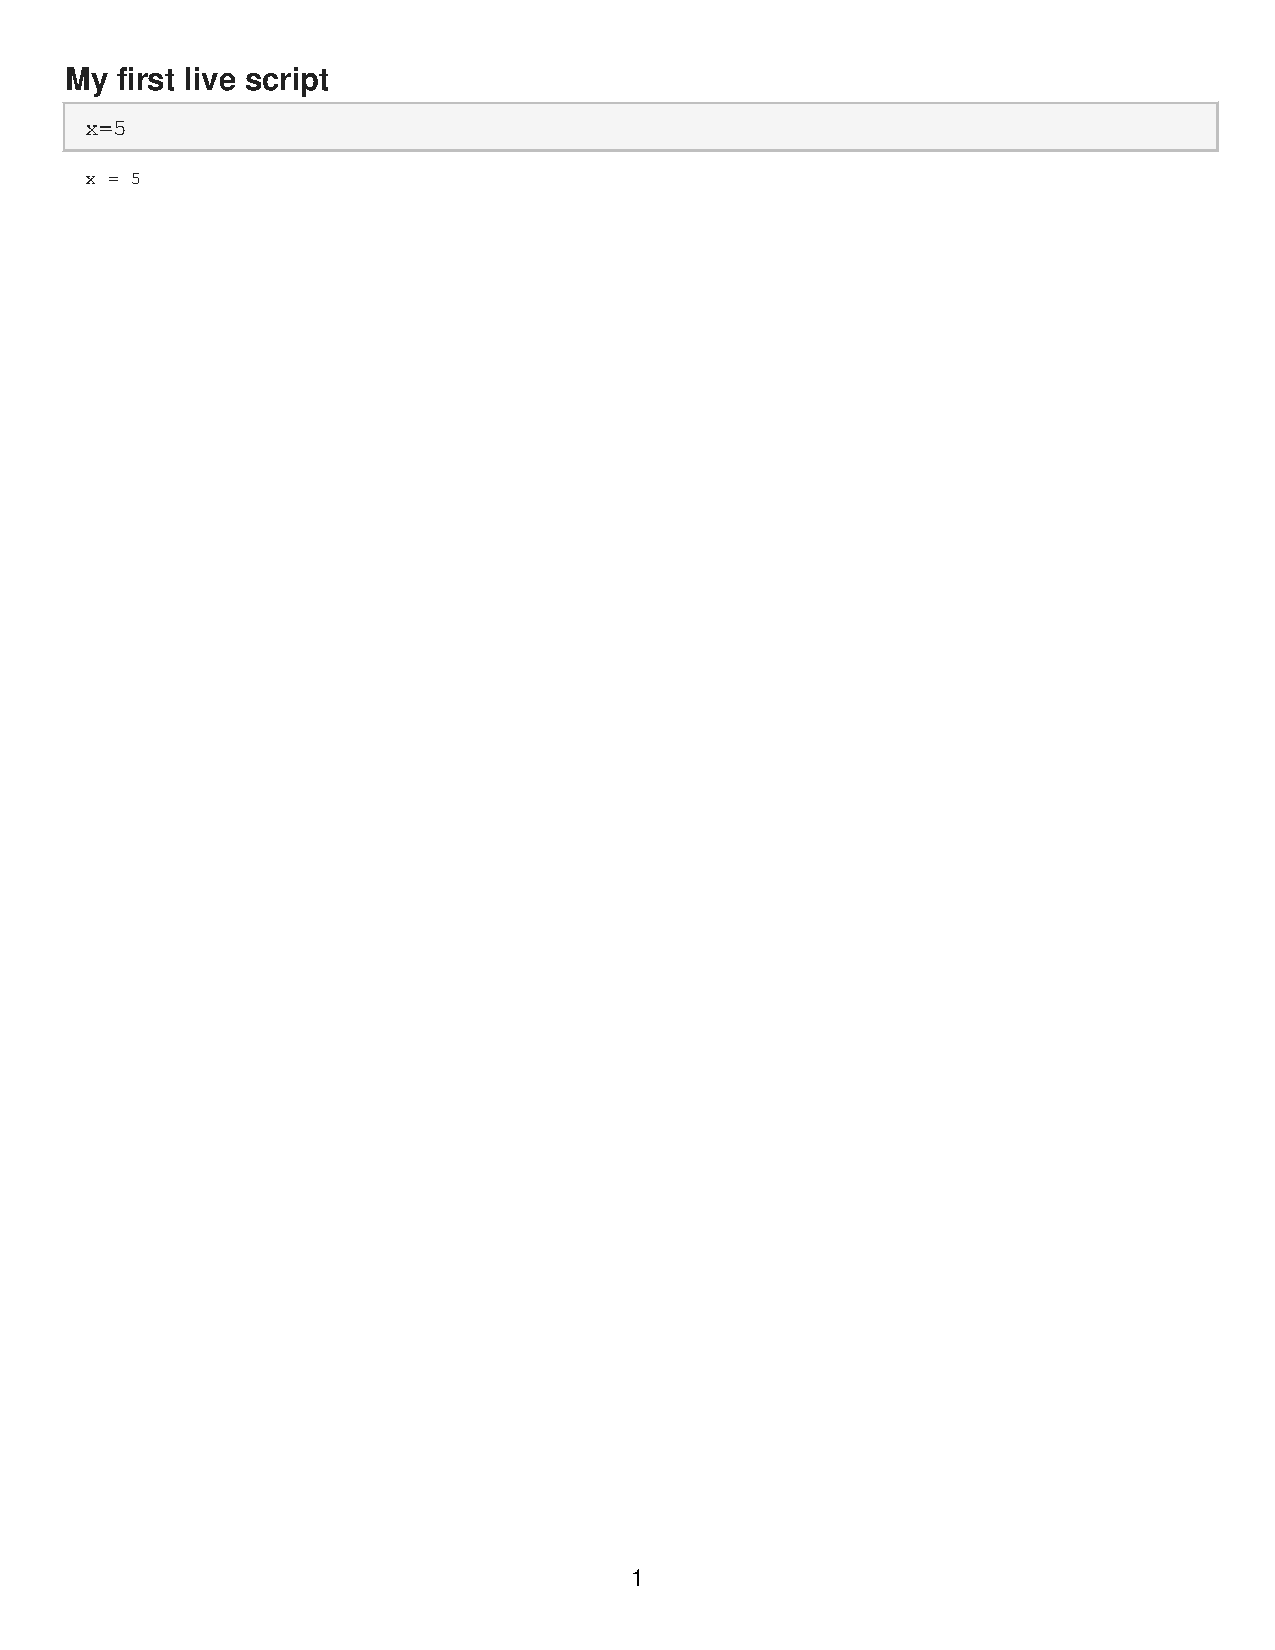
\includepdf[pages=-,frame,pagecommand={},width=0.9\textwidth]{w03_modeling_scripts/lessons/mylivescript.pdf}

\section{Chapter Review}

This chapter presented scripts and live scripts, suggesting reasons to use them.  We computed elements of a Fibonacci sequence, but because we used floating-point numbers, the results were sometimes only approximate.
And we saw how to add comments to a program to document what it does and explain how it works.

Here are some terms from this chapter you might want to remember.

An \emph{M-file} is a file that contains a \emph{script}, which is a sequence of MATLAB commands.
An \emph{MLX-file} is a file that contains a \emph{live script}, which is a collection of MATLAB code, rich text and graphics.
The \emph{search path} is the list of folders where the interpreter looks for
M-files.

A \emph{precondition} is something that must be true when the script
starts in order for it to work correctly; a \emph{postcondition} is something that will be true when the script completes.

The \emph{target} of an assignment statement is the variable on the left side.

\emph{Floating-point} is a way to represent and store numbers in a computer.
\mbox{\emph{Scientific notation}} is a format for typing and displaying large
and small numbers; for example, \lstinline{3.0e8} represents $3.0 \times 10^8$
or 300,000,000.

A \emph{comment} is part of a program that provides additional information
about the program, but does not affect its execution.

In the next chapter, you'll learn how to write programs that perform repetitive tasks using loops.


\section{Exercises}

Before you go on, you might want to work on the following exercises.

\begin{ex}
To test your understanding of assignment statements, write a few lines of code that swap the values of \lstinline{x} and \lstinline{y}.
Put your code in a script called \emph{swap.m} and test it.

If it works correctly, you should be able to run it like this:

\begin{code}
>> x = 1, y = 2
x = 1
y = 2

>> swap

>> x, y
x = 2
y = 1
\end{code}
\end{ex}

\begin{ex}
\label{bikegame}
\index{bike share system}

Imagine that you are the operator of a bike-share system with two
locations: Monterey and Pacific Grove.

You observe that every day 5 percent
of the bikes in Monterey are dropped off in Pacific Grove, and 3 percent of the bikes
in Pacific Grove get dropped off in Monterey.
At the beginning of the month, there are 100 bikes at each location.

Write a script called \emph{bike\textunderscore update.m} that updates the number
of bikes in each location from one day to the next.  The precondition
is that the variables \lstinline{m} and \lstinline{pg} contain the number of bikes
in each location at the beginning of the day.  The postcondition
is that \lstinline{m} and \lstinline{pg} have been modified to reflect the net movement of bikes.

To test your program, initialize \lstinline{m} and \lstinline{pg} at
the command prompt, then execute the script.  
\begin{code}
>> m = 100
>> pg = 100
>> bike_update
\end{code}

The script should display
the updated values of \lstinline{m} and \lstinline{pg}, but not any intermediate
variables.

Remember that bikes are countable things, so \lstinline{m} and \lstinline{pg} should always be integer values.  You might want to use the \lstinline{round} function
to compute the number of bikes that move each day.

If you execute your script repeatedly, you can simulate the passage
of time from day to day (you can repeat a command by pressing the \keycap{up} arrow and then \keycap{enter} - or by clicking the "Run" button repeatedly in the MATLAB editor).

What happens to the bikes?  Do they all end up in one place?  Does the system reach an equilibrium, does it oscillate, or does it do something else?

In the next chapter, we will see how to execute your script automatically
and how to plot the values of \lstinline{m} and \lstinline{pg} over time.

\end{ex}


\chapter{Loops}
\label{loops}


The programs we have seen so far are \emph{straight-line code}; that is, they execute one instruction after another from top to bottom.
This chapter introduces one of the most important programming-language features, the \lstinline{for}~loop, which allows simple programs to perform complex, repetitive tasks. This chapter also introduces the mathematical concepts of sequence and series, and a process for writing programs, incremental development.

We'll start by reviewing the exercise from the previous chapter; if you didn't do it, you might want to take a look before you go on.

\section{Updating Variables}

In Exercise~\ref{bikegame}, I asked you to write a program that models a bike-share system with bikes moving between two stations.
Each day 5 percent of the bikes in Monterey are dropped off in Pacific Grove, and 3 percent of the bikes
in Pacific Grove get dropped off in Monterey.

To update the state of the system, you might have been tempted to write something
like

\index{bike share system}

\begin{code}
m = m - 0.05*m + 0.03*pg
pg = pg + 0.05*m - 0.03*pg
\end{code}

But that would be wrong, so very wrong.  Why?  The problem is that
the first line changes the value of \lstinline{m}, so when the second line
runs, it gets the old value of \lstinline{pg} and the new value of \lstinline{m}.
As a result, the change in \lstinline{m} is not always the same as the
change in \lstinline{pg}, which violates the Principle of Conservation
of Bikes!

One solution is to use temporary variables like \lstinline{m_new} and \lstinline{pg_new}:

\begin{code}
m_new = m - 0.05*m + 0.03*pg
pg_new = pg + 0.05*m - 0.03*pg
m = m_new
pg = pg_new
\end{code}

This has the effect of updating the variables \emph{simultaneously}; that
is, it reads both old values before writing either new value.

\index{update}

The following is an alternative solution that
has the added advantage of simplifying the computation:

\begin{code}
m_to_pg = 0.05*m - 0.03*pg
m = m - m_to_pg
pg = pg + m_to_pg
\end{code}

It's easy to look at this code and confirm that it obeys Conservation
of Bikes.  Even if the value of \lstinline{m_to_pg} is wrong, at least the total
number of bikes is right.  And that brings us to the Fifth Theorem of
Debugging:\index{debugging!Fifth Theorem}

\begin{quote}
The best way to avoid a bug is to make it impossible.
\end{quote}

In this case, removing redundancy also eliminates the opportunity for  a bug.

\section{Bug Taxonomy}

The more you understand bugs, the better you will be at debugging. Here are a few common types of bus:

\index{syntax error}
\index{runtime error}
\index{logical error}
\index{numerical error}

\begin{description}

\item[Syntax error] You have written a command that cannot execute because it violates one of the language's syntax rules.  For example, in MATLAB, you can't have two operands in a row without an operator, so \lstinline{pi r^2} contains a syntax error, or you could forget the closing parenthesis.  When the interpreter finds a syntax error, it prints an error message and stops running your program.\index{error!syntax}

\item[Runtime error] Your program starts running, but something goes wrong along the way.  For example, if you try to access a variable that doesn't exist, that's a runtime error.  Division by zero is another example.  When the interpreter detects the problem, it prints an error message and stops.\index{error!runtime}

\item[Logical error] Your program runs without generating any error messages, but it doesn't do what you intended.  The problem in the previous section, where we changed the value of \lstinline{b} before reading the old value, is a logical error.\index{error!logical}  Logical errors include some specific subspecies:
\begin{description}
    \item [Semantic error] The meaning inherent in the program is different from your intended meaning.  For example, your use the command \lstinline{sin(90)}, expecting MATLAB to interpret that as the sine of a \SI{90}{\degree} angle, but MATLAB returns 0.894 because the function expects the argument in radians.
    \item [Type error] Errors involving incompatible data types.  We'll see examples of this later, such as trying to add a string (letters) to numbers.
    \item[Numerical error] Most computations in MATLAB are only approximately right.  Most of the time the errors are small enough that we don't care, but in some cases the round-off errors are a problem.\index{error!numerical}
\end{description}
\end{description}

Syntax errors are usually the easiest to deal with because you will get timely feedback on the error; the code simply won't run until they are fixed.  Sometimes the error messages are confusing, but MATLAB can usually tell you where the error is, at least roughly.  The MATLAB Editor can even continuously check your code before you try to execute, similar to automated spell-check when writing a document.

Runtime errors a little harder because, as I mentioned before, MATLAB can tell you where it detected the problem, but often not what caused it.

Logical errors, akin to the \href{https://en.wikipedia.org/wiki/Garbage_in,_garbage_out}{garbage in, garbage out} concept, are hard because MATLAB can't help at all. From MATLAB's point of view there's nothing wrong with the program; only you know what the program is supposed to do, so only you can check it.  These errors are usually detected only through deliberate testing to execute the program, or parts of the program, when you have a clear way to verify that the actual behavior matches the intended outcome.

Semantic errors are best avoided at design time by reading the documentation about the commands you are using so that you are interpreting them the same way that MATLAB expects and writing down your models before implementing them in a program.

Numerical errors can be tricky because it's not clear whether the problem is your fault.  For most simple computations, MATLAB produces the floating-point value that is closest to the exact solution, which means that the first 15 significant digits should be correct.

But some computations are ill-conditioned, which means that even if your program is correct, the round-off errors accumulate and the number of correct digits can be smaller.  Sometimes MATLAB can warn you that this is happening, but not always!  \emph{Precision} (the number of digits in the answer) does not imply \emph{accuracy} (the number of digits that are right).


\section{Absolute and Relative Error}

There are two ways of thinking about numerical errors.
The first is \emph{absolute error}, or the difference between the correct value and the approximation.  We often write the magnitude of the error,
ignoring its sign, when it doesn't matter whether the approximation
is too high or too low.
\index{error!absolute} \index{absolute error}

The second way to think about numerical errors is \emph{relative error}, where the error is expressed as a fraction (or percentage) of the exact value.\index{error!relative}
\index{relative error}

For example, we might want to estimate $9!$ using the formula
$\sqrt {18 \pi} ( 9 / e)^9$.  The exact answer is $9 \cdot 8 \cdot 7 \cdot 6
\cdot 5 \cdot 4 \cdot 3 \cdot 2 \cdot 1 = 362,880$.  The approximation
is $359,536.87$.  So the absolute error is $3,343.13$.

At first glance, that sounds like a lot---we're off by three
thousand---but we should consider the size of the
thing we are estimating.  For example, \$3,000 matters a lot
if we're talking about an annual salary, but not at all if we're talking about the national debt.

A natural way to handle this problem is to use relative
error.
In this case, we would divide the error
by $362,880$, yielding $0.00921$, which is just less than 1 percent.
For many purposes, being off by 1 percent is good enough.


\section{for Loops}

\index{for loop@\lstinline{for} loop}
\index{loop}

Let's return to the bike-share example.
In the previous chapter, we wrote a \emph{bike\textunderscore update.m} script to simulate a
day in the life of a bike-share system. To simulate an entire
month, we'd have to run the script 30 times. We could enter the same command 30 times, but it's simpler to use a \emph{loop}, which is a set of statements that executes repeatedly.

To create a loop, we can use the \lstinline{for} statement, like this:

\begin{code}
for i=1:30
    bike_update
end
\end{code}

The first line includes what looks like an assignment statement, and it \emph{is}
like an assignment statement, except that it runs more than once.  The
first time, it creates the variable \lstinline{i} and assigns it the
value~1.  The second time, \lstinline{i} gets the value~2, and so on, up to
and including 30.

\index{assignment statement}
\index{statement!assignment}
\index{colon operator}
\index{operator!colon}
\index{range}

The colon operator (\lstinline{:}) specifies a \emph{range} of integers.
You can create a range at the prompt:

\begin{code}
>> 1:5
ans =  1     2     3     4     5
\end{code}

The variable you use in the \lstinline{for} statement is called the \emph{loop
variable}.  It's common to use the names \lstinline{i},
\lstinline{j}, and \lstinline{k} as loop variables.

\index{body of loop}
\index{loop body}
\index{loop variable}
\index{variable!loop}

The statements inside the loop are called the \emph{body}.  By convention,
they are indented to show that they're inside the loop, but the
indentation doesn't affect the execution of the program.
The \lstinline{end} statement marks the end of the loop.

\index{end statement@\lstinline{end} statement}
\index{statement!end@\lstinline{end}}

To see a loop in action you can run one that displays the
loop variable:

\begin{code}
>> for i=1:5
    i
end

i = 1
i = 2
i = 3
i = 4
i = 5
\end{code}

As this example shows, you \emph{can} run a \lstinline{for} loop from the
command line, but it's more common to put it in a script.

\begin{ex}
Create a live script named \emph{bike\textunderscore loop.mlx} that does the following:
\begin{enumerate}
\item Assign the initial values (precondition) of \textbf{\lstinline{m = 100}} and \textbf{\lstinline{pg = 100}}.
\item Run the \lstinline{for} loop from 1 to 30.
\begin{enumerate}
    \item Inside the loop, call the program \emph{bike\textunderscore update.m} to update the values of \lstinline{m} and \lstinline{pg}.  The program should echo the values of \lstinline{m} and \lstinline{pg} after each update.
\end{enumerate}
\end{enumerate}

If everything goes smoothly, your script will display a long stream
of numbers on the screen.  It's probably too long
to fit, and even if it did fit, it would be hard to interpret.
A graph (coming soon) would be much better!
\end{ex}



\section{Plotting}
\label{plotting}

\index{plot@\lstinline{plot}}

If the output of your program is a long stream of numbers, it can be hard to see what is happening.
Plotting the results can make things clearer.

The \lstinline{plot} function is a versatile tool for plotting two-dimensional graphs.  Unfortunately, it's so versatile that it can be hard to use (and hard to read the documentation).
We'll start simple and work our way up.

To plot a single point, type

\begin{code}
>> plot(1, 2, 'o')
\end{code}

A Figure Window should appear with a graph and a single blue circle at $x$ position 1 and $y$ position 2.

\index{Figure Window}
\index{style string}

The letter in single quotes is a \emph{style string} that specifies how the
point should be plotted;  \lstinline{o} indicates a circle.
Other shapes include \lstinline{+},
\lstinline{*},
\lstinline{x},
\lstinline{s} (for a square),
\lstinline{d} (for a diamond), and
\lstinline{^} (for a triangle).

You can also specify the color by starting the style string with a color code:

\begin{code}
>> plot(1, 2, 'ro')
\end{code}

Here, \lstinline{r} stands for red; the other colors include \lstinline{g} for green, \lstinline{b} for blue, \lstinline{c} for cyan, \lstinline{m} for magenta, \lstinline{y} for yellow, and \lstinline{k} for black.

When you use \lstinline{plot} this way, it can only plot one point at a
time.  If you run \lstinline{plot} again, it clears the figure before making
the new plot.  The \lstinline{hold}~command lets you override that behavior:
\lstinline{hold on} tells MATLAB not to clear the figure when it makes a new
plot; \lstinline{hold off} returns to the default behavior.

\index{hold@\lstinline{hold}}

Try this:

\begin{code}
>> clf
>> hold on
>> plot(1, 1, 'ro')
>> plot(2, 2, 'go')
>> plot(3, 3, 'bo')
>> xlabel('x axis label [units]')
>> ylabel('y axis label [units]')
>> hold off
\end{code}

The \lstinline{clf} command clears the figure before we start plotting.

\index{clear figure}
\index{clf@\lstinline{clf}}

If you run the code above, you should see a figure with three circles and text labels on the axes similar to Figure~\ref{fig:ex}.  MATLAB scales the plot automatically so that the axes run from the lowest values in the plot to the highest.

\begin{figure}[h]
    \centerline{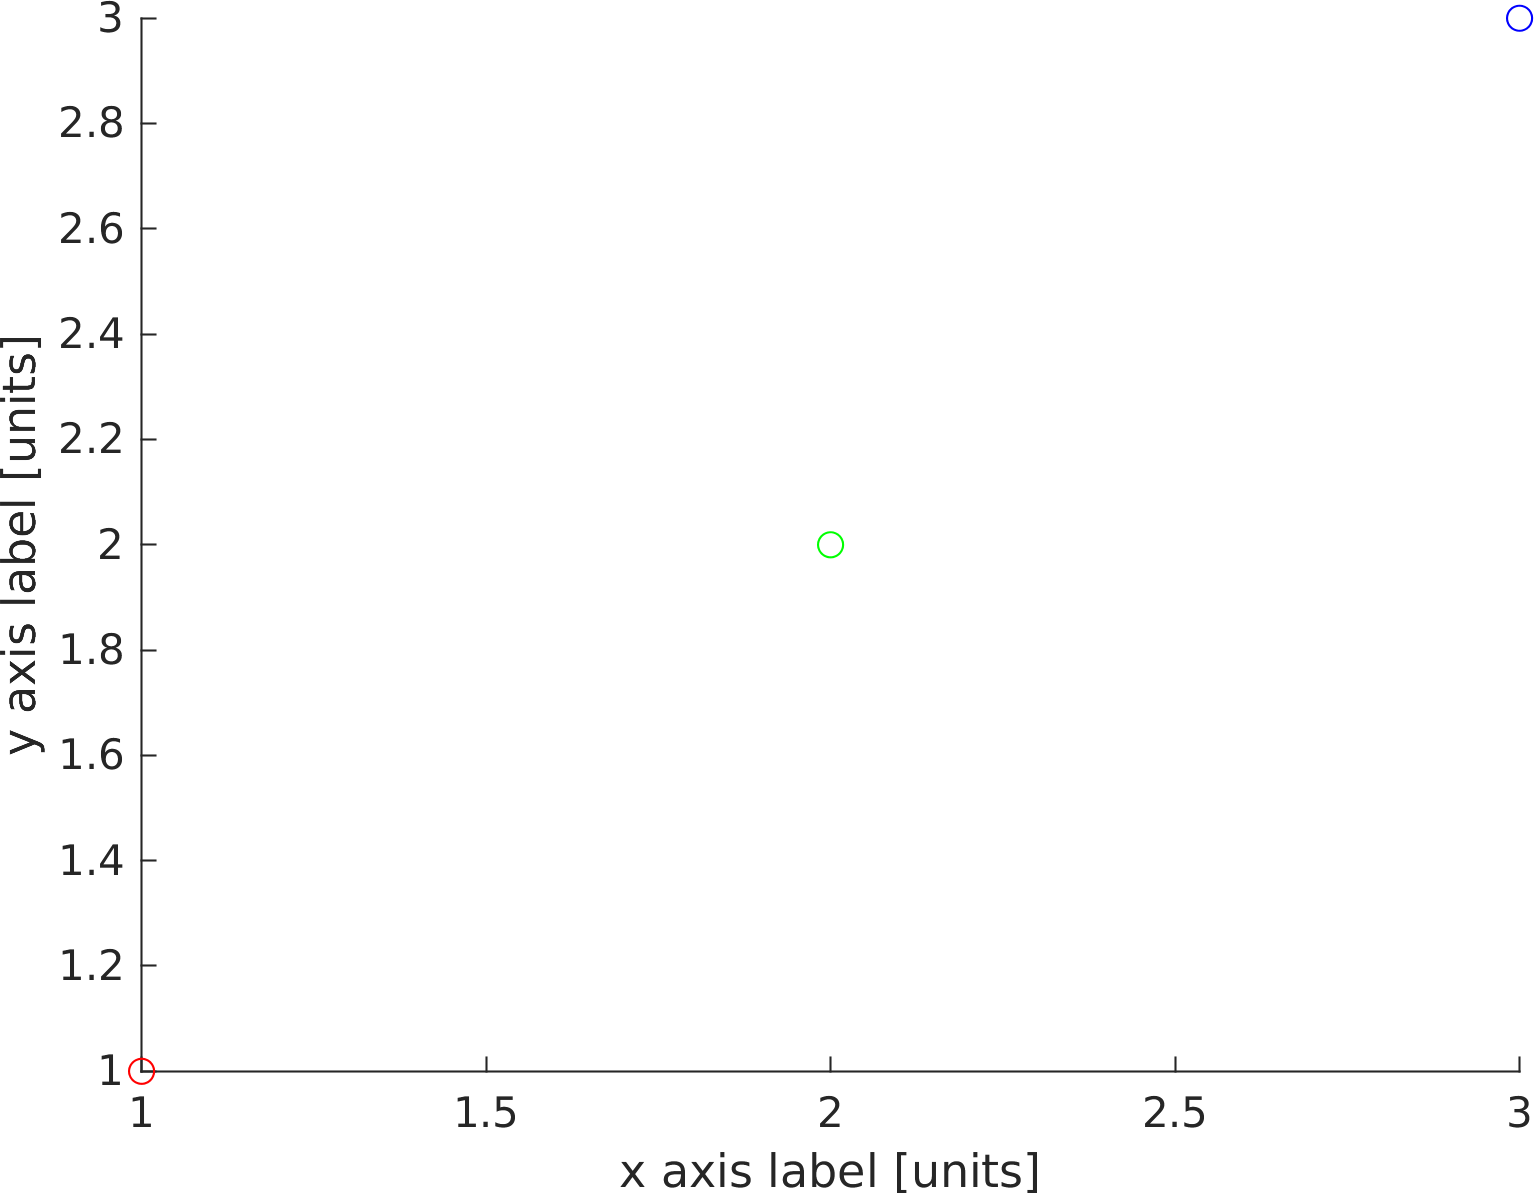
\includegraphics[scale=0.8]{images/fig03_ex.png}}
    \caption{Simple figure with three markers and axes labels.}
    \label{fig:ex}
\end{figure}

\begin{ex}
Using \emph{bike\textunderscore loop.mlx} as a starting point, develop a live script \emph{bike\textunderscore loop\textunderscore plot.mlx} so that it clears the figure before running the loop.  Then, each time through the loop, it should plot the value of \lstinline{m} versus the value of \lstinline{ii} with a red circle.

Once you get that working, modify it so it plots the values of \lstinline{pg} with blue diamonds.
\end{ex}


\section{Sequences}

Now that we have the ability to write loops, we can use them to explore sequences and series, which are useful for describing and analyzing systems that change over time.

In mathematics, a \emph{sequence} is a set of numbers that corresponds to the positive integers.  The numbers in the sequence are called \emph{elements}.  In math notation, the elements are denoted with subscripts, so the first element of the series $A$ is
$A_1$, followed by $A_2$, and so on.

\index{sequence}
\index{element}
\index{loop}
\index{geometric sequence}

A \lstinline{for} loop is a natural way to compute the elements of a sequence. As an example, in a \href{https://en.wikipedia.org/wiki/Geometric_progression}{geometric sequence}, each element is a constant multiple of the previous element.  Expressed mathematically, element $i+1$ (the next element) of the sequence can be expressed as the product of the element $i$ (the previos element) and the constant \emph{common ratio}, $r$ or
\begin{equation*}
A_{i+1} = A_{i} r.
\end{equation*}

As a more specific example, let's
look at the sequence with $A_1 = 1$ and $r=1/2$ so that the relationship $A_{i+1} = A_i/2$, for all $i$.  In other words, each element is half as big as the one before it.

The following loop computes the first 10 elements of $A$:

\begin{code}
a = 1
r = 1/2
for ii = 2:10
    a = a * r
end
\end{code}

The first line initializes the variable \lstinline{a} with the first element of the sequence, $A_1$. Each time through the loop, we find the next value of \lstinline{a}
by dividing the previous value by~2, and assign the result back to \lstinline{a}.
At the end, \lstinline{a} contains the 10th element.  The reason we use the variable \lstinline{ii} instead of just \lstinline{i} is that MATLAB defines bot \lstinline{i} and \lstinline{j} as complex numbers, so using either as a variable causes a naming collision that may be tough to debug.

The other elements are displayed on the screen, but they are not saved in a variable.
Later, we'll see how to store the elements of a sequence in a vector.

\index{direct computation}
\index{recurrent computation}

This loop computes the sequence \emph{recurrently}, which means that each element depends on the previous one. For this sequence, it's also possible to compute the $i$th element \emph{directly}, as a function of $ii$, without using the previous element. In math notation, $A_i = A_1 r^{ii-1}$.

\begin{ex}
Write a script named \emph{sequence.m} that uses a loop to
compute elements of $A$ \mbox{directly}.
\end{ex}

\section{Series}
\label{series}

In mathematics, a \emph{series} is the sum of the elements of a sequence.  It's a terrible name, because in common English, ``sequence'' and ``series'' mean pretty much the same thing, but in math, a sequence is a set of numbers, and a series is an expression (a sum) that has a single value.  In math notation,  a series is often written using the summation symbol $\sum$.

\index{series}
\index{sum}

For example, the sum of the first 10 elements of $A$ is
\begin{equation*}
\sum_{i=1}^{10} A_i
\end{equation*}

A \lstinline{for} loop is a natural way to compute the value of this series:

\begin{lstlisting}[caption={A program that calculates a simple series}, label={lst:series_10}]
A1 = 1;
total = 0;
for ii = 1:10
    a = A1 * (1/2)^(ii-1);
    total = total + a;
end
ans = total
\end{lstlisting}

Let's walk through what's happening here. \lstinline{A1} is the first element of the sequence, so we assign it to be \lstinline{1}; we also create \lstinline{total}, which will store the cumulative sum.
Each time through the loop, we set \lstinline{a} to the $i$th element and add \lstinline{a} to the \lstinline{total}.
At the end, outside the loop, we store  \lstinline{total} as \lstinline{ans}.

The way we're using \lstinline{total} is called an \emph{accumulator}, that is, a variable that accumulates the result a little bit at a time.
\index{accumulator}



\begin{ex}
This example computes the terms of the series directly. As
an exercise, write a script named \emph{series.m} that computes
the same sum by computing the elements recurrently.  You will
have to be careful about where you start and stop the loop.
\end{ex}


\section{Generalization}

\index{generalization}

As written, the previous example always adds up the first 10
elements of the sequence, but we might be curious to know what
happens to \lstinline{total} as we increase the
number of terms in the series.  If you've studied geometric
series, you might know that this series converges on~2; that is,
as the number of terms goes to infinity, the sum approaches~2 asymptotically.

To see if that's true for our program, we can replace the
constant \lstinline{10} in Listing~\ref{lst:series_10} with a variable named \lstinline{n}:

\begin{lstlisting}[caption={Updating our code from Listing~\ref{lst:series_10} to have a variable number of terms}, label={lst:series_n}]
A1 = 1;
total = 0;
for i=1:n
    a = A1 * (1/2)^(i-1);
    total = total + a;
end
ans = total
\end{lstlisting}

The code in Listing~\ref{lst:series_n} can now compute any number of terms, with the
precondition that you have to set \lstinline{n} before you execute
the code.
I put this code in a file named \emph{series.m}, then
ran it with different values of \lstinline{n}:

\begin{code}
>> n=10; series
total = 1.99804687500000

>> n=20; series
total = 1.99999809265137

>> n=30; series
total = 1.99999999813735

>> n=40; series
total = 1.99999999999818
\end{code}

It sure looks like it's converging on 2.

Replacing a constant with a variable is called \emph{generalization}.
Instead of computing a fixed, specific number of terms, the new script
is more general; it can compute any number of terms.
This is an important idea we'll come back to when we talk about functions.

\section{Incremental Development}

\index{incremental development}

As you start writing longer programs, you might find yourself spending more time debugging.
The more code you write before you start debugging, the harder it is to find
the problem.

\emph{Incremental development} is a way of programming that tries
to minimize the pain of debugging by developing and testing in small steps.  The fundamental steps are:

\begin{enumerate}

\item Always start with a working program.  If you have an
example from a book, or a program you wrote that is similar to
what you are working on, start with that.  Otherwise, start with
something you \emph{know}  is correct, like \lstinline{x = 5}.  Run the program
and confirm that you are running the program you think you are
running.
This step is important, because in most environments there
are little things that can trip you up when you start a new
project.  Get them out of the way, so you can focus on programming.

\item Make one small, testable change at a time.  A \emph{testable}
change is one that displays something on the screen (or has some
other effect) that you can check.  Ideally, you should know what
the correct answer is or be able to check it by performing another
computation.

\item Run the program and see if the change worked.  If so, go back
to step~2.  If not, you'll have to do some debugging, but if the
change you made was small, it shouldn't take long to find the problem.

\end{enumerate}

\index{debugging!Sixth Theorem}

With incremental development, your code is more likely to work the first time, and if it doesn't, the problem is more likely to be obvious.  And that brings us to the Sixth Theorem of Debugging:

\begin{quote}
The best kind of debugging is the kind you don't have to do.
\end{quote}

In practice, there are two problems with incremental development.
First, sometimes you have to write extra code to
generate visible output that you can check.  This extra code is
called \emph{scaffolding} because you use it to build the program
and then remove it when you are done.  But the time you save on
debugging is almost always worth the time you invest in
scaffolding.
\index{scaffolding}

The second problem is that when you're getting started, you might not know how to
choose steps that get from \lstinline{x = 5} to the program you're trying
to write.  We'll look at an extended example in Chapter~6.

If you find yourself writing more than a few lines of code before
you start testing, and you're spending a lot of time debugging,
you should try incremental development.




\section{Chapter Review}

In this chapter, we used a loop to perform a repetitive computation---updating a model 30 times---and to compute sequences and series.  Also,  we used the \lstinline{plot} function to visualize the results.

Here are some terms from this chapter you might want to remember.

\emph{Absolute error} is the difference between an approximation and
an exact answer. \emph{Relative error} is the same difference expressed as a fraction or percentage of the exact answer.

A \emph{loop} is part of a program that runs repeatedly.
A \emph{loop variable} is a variable that gets assigned a different value each time through the loop.
A \emph{range} is a sequence of values assigned to the loop variable, often
specified with the colon operator---for example, \lstinline{1:5}.
The \emph{body} of a loop is the set of statements inside the loop that runs repeatedly.
An \emph{accumulator} is a variable that is used to accumulate a result a little bit at a time.

In mathematics, a \emph{sequence} is a set of numbers that correspond
to the positive integers.
The numbers that make up the sequence are called \mbox{\emph{elements}}.
A \emph{series} is the sum of a sequence of elements.
Sometimes we compute the elements of a sequence \emph{recurrently}, which means that each new element depends on previous elements.  Sometimes we can compute the elements \emph{directly}, without using previous elements.

\emph{Generalization} is a way to make a program more versatile, for example, by replacing a specific value with a variable that can have any value.
\emph{Incremental development} is a way of programming by making a series of small, testable changes.
\emph{Scaffolding} is code you write to help you program or debug, but
that is not part of the finished program.

In the next chapter, we'll use a vector to store the results from a loop.


\section{Exercises}

Before you go on, you might want to work on the following exercises.

\begin{ex}
Years ago I was in a fudge shop and saw a sign that said ``Buy one pound of fudge, get another quarter pound free.''  That's simple enough.

But if I ran the fudge shop, I would offer a special deal to anyone who could solve the following problem:

\begin{quote}
If you buy a pound of fudge, we'll give you another quarter pound free.  And then we'll give you a quarter of a quarter pound, or one-sixteenth.  And then we'll give you a quarter of that, and so on.  How much fudge would you get in total?
\end{quote}

Write a script called \emph{fudge.m} that solves this problem.  Hint: start with \emph{series.m} and generalize it by replacing the ratio \lstinline{1/2} with a variable, \lstinline{r}.

% fudge.m
\end{ex}




\begin{ex}
\label{fib2}

We have already seen the Fibonacci sequence, $F$, which
is defined recurrently as

\[ \mathrm{for}~i \ge 3, \quad  F_{i} = F_{i-1} + F_{i-2} \]

In order to get started, you have to specify the first two
elements, but once you have those, you can compute the rest.
The most common Fibonacci sequence starts with $F_1 = 1$ and $F_2 = 1$.

Write a script called \emph{fibonacci2.m} that uses a \lstinline{for} loop
to compute the first 10 elements of this Fibonacci sequence.
As a postcondition, your script should assign the 10th element to
\lstinline{ans}.

Now generalize your script so that it computes the $n$th element
for any value of \lstinline{n}, with the precondition that you have to
set \lstinline{n} before you run the script.  To keep things simple for
now, you can assume that \lstinline{n} is greater than~0.

Hint: you'll have to use two variables to keep track of the
previous two elements of the sequence.  You might want to call
them \lstinline{prev1} and \lstinline{prev2}.  Initially, \lstinline{prev1} = $F_1$
and \lstinline{prev2} = $F_2$.  At the end of the loop, you'll have
to update \lstinline{prev1} and \lstinline{prev2}; think carefully about the
order of the updates!

\end{ex}

\chapter{Vectors}
\label{vectors}

In the previous chapter we used a loop to compute the elements (scalars) of a sequence, but we were only able to store the last element.  In this chapter, we'll use a vector to store all the elements in an array.
We'll also learn how to select elements from a vector, and how to perform vector arithmetic and common vector operations like \emph{reduce} and \emph{apply}.

\section{Creating Vectors}

\index{vector}

A \emph{vector} in MATLAB is a sequence of numbers, stored as an array.
There are several ways to create vectors; one of the most common is
to put a sequence of numbers in square brackets:

\begin{code}
>> [1 2 3]
ans = 1     2     3
\end{code}

The \lstinline{size} function tells you the number of elements in each dimension.

\begin{code}
>> size(xx)
ans =
    1     3
\end{code}
This indicates that \lstinline{xx} is a 1-by-3 array.  We will learn later that this is a \emph{row} vector.


Another way to create a vector is the colon operator, which we have already used to create a range of values in a \lstinline{for} loop.

\begin{code}
>> 1:3
ans = 1     2     3
\end{code}

In general, anything you can do with a number, you can also do with
a vector.  For example, you can assign a vector value to a variable:

\begin{code}
>> xx = [1 2 3]
X = 1     2     3
\end{code}

Note that variables that contain vectors are often double letters (\lstinline{xx}) or capital letters (\lstinline{X}).
These are just conventions; MATLAB doesn't require it, but it's a useful way to remember which variables are vectors.

Here are the syntax for some typical ways to create a vector:
\begin{code}
     % Some ways to initialize vectors
     % As an list with step size = 1
     1:5
     ans =
          1     2     3     4     5

     % As a list with step size ~= 1
     1:3:10
     ans =
          1     4     7    10

     % As an N-by-1 column of zeros
     zeros(5,1)
     ans =
          0
          0
          0
          0
          0

     % As a 1-by-N row of ones
     ones(1,5)
     ans =
          1     1     1     1     1

     % A vector of psuedorandom numbers
     rand(1,5)
     ans =
         0.1576    0.9706    0.9572    0.4854    0.8003

     % Manually, as a row vector
     [5 3.1 9.8 -2]
     ans =
         5.0000    3.1000    9.8000   -2.0000

     % Manually as a column vector
     [5; 3.1; 9.8; -2;]
     ans =
         5.0000
         3.1000
         9.8000
        -2.0000

     % As a column using transpose
     [5 3.1 9.8 -2]'
     ans =
         5.0000
         3.1000
         9.8000
        -2.0000

     % Linear spacing from A to B with N elements
     linspace(0, 1, 5)
     ans =
            0    0.2500    0.5000    0.7500    1.0000
        
     % Logrithmic spacing from A to B with N elements
     logspace(0, 1, 5)
     ans =
       1.0000    1.7783    3.1623    5.6234   10.0000
\end{code}

\index{variable}

\section{Vector Arithmetic}
\label{elementwise}

\index{vector arithmetic}
\index{arithmetic!vector}

As with numbers, you can do arithmetic with vectors.  However, operations with vectors can be done in more than one way, so to avoid logical errors, we need to be more intentional with the instructions we provide.  In general, MATLAB executes both \emph{array operations} and \emph{matrix operations}.   Matrix operations follow the rules of linear algebra, while array operations execute element by element.  The syntax for each can be closely related.


If you add a scalar to a vector, MATLAB does the array operation increments each element of the vector:

\begin{code}
>> Y = X + 5
Y = 6     7     8
\end{code}

The result is a new vector; the original value of \lstinline{X} has not
changed.

If you add two vectors, MATLAB adds the corresponding elements of each
vector and creates a new vector that contains the sums:

\begin{code}
>> Z = X + Y
Z = 7     9    11
\end{code}

But adding vectors only works if the operands are the same size.
Otherwise, you get an error:

\begin{code}
>> W = [1 2]
W = 1     2

>> X+W
Arrays have incompatible sizes for this operation.
Related documentation 
\end{code}

The \lstinline(size()) function can be helpful in debugging runtime errors of vector/matrix sizing, e.g.,
\begin{code}
    >> size(X)
    ans =
         1     3
    >> size(W)
    ans =
         1     2
\end{code}
might help us investigate whey we received the `Matrix dimensions must agree' error.

\index{matrix}
\index{elementwise operator}
\index{operator!elementwise}

If you divide two vectors, you might be surprised by the result:

\begin{code}
>> X / Y
ans = 0.2953
\end{code}

MATLAB is performing a matrix operation called right-matrix division, which is not what we expected.  (See the \lstinline{mrdivid()} function documentation for more details.)
If, instead, we wanted MATLAB to do the array operation o divide the elements of \lstinline{X} by the elements of \lstinline{Y}, you have to use \lstinline{./}, which is element-wise division:

\begin{code}
>> X ./ Y
ans = 0.1667    0.2857    0.3750
\end{code}

Multiplication has the same problem.  If you use \lstinline{*}, MATLAB does matrix multiplication following the rules of linear algebra.  With these two vectors, matrix multiplication is not defined, so you get an error:

\begin{code}
>> X * Y
Error using  *
Incorrect dimensions for matrix multiplication.
Check that the number of columns in the first matrix
matches the number of rows in the second matrix.
To perform element-wise multiplication, use '.*'.
\end{code}

In this case, the error message is pretty helpful.  As it suggests, you can use \lstinline{.*} to perform element-wise multiplication:

\index{matrix multiplication}
\index{multiplication!matrix}

\begin{code}
>> X .* Y
ans = 6    14    24
\end{code}

As an exercise, see what happens if you use the exponentiation operator
(\lstinline{^}) with a vector.

\section{Indexing and Slicing}

In MATLAB, array \emph{indexing} refers to accessing specific elements of an array using their position, while \emph{slicing} allows selecting multiple elements, such as a range of rows, columns, or both.  MATLAB uses 1-based indexing, meaning the first element is at position 1. To access an element, you specify its index in parentheses. For example, for vector \lstinline{Y}:

\index{element}
\index{parentheses}


\begin{code}
>> Y = [6 7 8 9]
Y = 6    7     8     9

>> Y(1)
ans = 6

>> Y(4)
ans = 9
\end{code}

This means that the first element of \lstinline{Y} is \lstinline{6} and the
fourth element is~\lstinline{9}.  
The number in parentheses is called the \emph{index} because it indicates which element of the vector you want.

\index{index}

The index can be a variable name or a mathematical expression:

\begin{code}
>> i = 1;
>> Y(i)
ans = 6
>> Y(i+1)
ans = 7
\end{code}

We can use a loop to display the elements of \lstinline{Y}:

\index{loop}

\begin{code}
for i=1:4
     Y(i)
end
\end{code}

Each time through the loop we use a different value of \lstinline{i}
as an index into~\lstinline{Y}.

\index{length function@\lstinline{length} function}
\index{function!\lstinline{length}}

In the previous example we had to know the number
of elements in \lstinline{Y}.  We can make it more general by using
the \lstinline{length} function, which returns the number of elements
in a vector:

\begin{code}
for i=1:length(Y)
     Y(i)
end
\end{code}

This version works for a vector of any length.

When slicing a vector, you can extract a subset of the array using colon notation \lstinline{:} to indicate ranges.
\begin{code}
    >> B = [1, 2, 3, 4, 5]
    B =
         1     2     3     4     5
    >> C = B(2:4)
    C =
         2     3     4
\end{code}

You can also slice a vector to extract the elements described by another vector:
\begin{code}
    >> D = B([2 5])
    D =
         2     5
\end{code}

\section{Indexing Errors}

\index{index}
\index{expression}

An index can be any kind of expression, but the value of the
expression has to be a positive integer, and it has to be
less than or equal to the length of the vector.  If it's
zero or negative, you'll get an error:

\begin{code}
>> Y(0)
Array indices must be positive integers or logical values.
\end{code}

If it's not an integer, you get an error:

\begin{code}
>> Y(1.5)
Array indices must be positive integers or logical values.
\end{code}

If the index is too big, you also get an error:

\begin{code}
>> Y(5)
Index exceeds the number of array elements (4).
\end{code}

The \lstinline{end} keyword can help with indexing and slicing.  It refers to the maximum index value, so that
\begin{code}
    >> Y(end)
    ans =
         8
\end{code}
will index the last element in the vector no matter how many elements are included.  This is particularly helpful when slicing the last N elements of a vector:
\begin{code}
    >> G = 1:10
    G =
         1     2     3     4     5     6     7     8     9    10
    >> N = 5
    N =
         5
    >> H = G(end-N:end)
    H =
         5     6     7     8     9    10
\end{code}

\section{Vectors and Sequences}
\label{vecseq}

\index{vector}
\index{sequence}
\index{Fibonacci}

Vectors and sequences go together nicely.
For example, another way to evaluate the Fibonacci sequence from Chapter~2 is to
store successive values in a vector.  Remember that the definition of the
Fibonacci sequence is $F_1 = 1$, $F_2 = 1$, and
$F_{i} = F_{i-1} + F_{i-2}$ for $i > 2$.

Listing~\ref{lst:fib_vec} shows how we can compute the elements of this sequence and store them in a vector, using a capital letter for the vector \lstinline{F}
and lower-case letters for the integers \lstinline{i} and \lstinline{n}.

\begin{lstlisting}[caption={Calculating the Fibonacci sequence using a vector}, label={lst:fib_vec}]
F(1) = 1
F(2) = 1
for i=3:n
    F(i) = F(i-1) + F(i-2)
end
\end{lstlisting}

If you had any trouble with \nameref{fib2}, you have to
appreciate the simplicity of this script.  The MATLAB syntax is
similar to the math notation, which makes it easier to check for
correctness.

If you only want the $n$th Fibonacci number, storing
the whole sequence wastes some space.  But if wasting space
makes your code easier to write and debug, that's probably okay.


\section{Plotting Vectors}

\index{plotting vector}
\index{vector!plotting}
\index{plot@\lstinline{plot}}

If you call \lstinline{plot} with a vector as an argument,
MATLAB plots the indices on the x-axis and the elements on the
y-axis.  To plot the Fibonacci numbers we computed in Listing~\ref{lst:fib_vec}, we'd use

\begin{code}
plot(F)
xlabel('Index [n/a]')
ylabel('Fibonacci number [n/a]')
\end{code}

Figure~\ref{fig:fibonacci} shows the result.

\begin{figure}[h]
\centerline{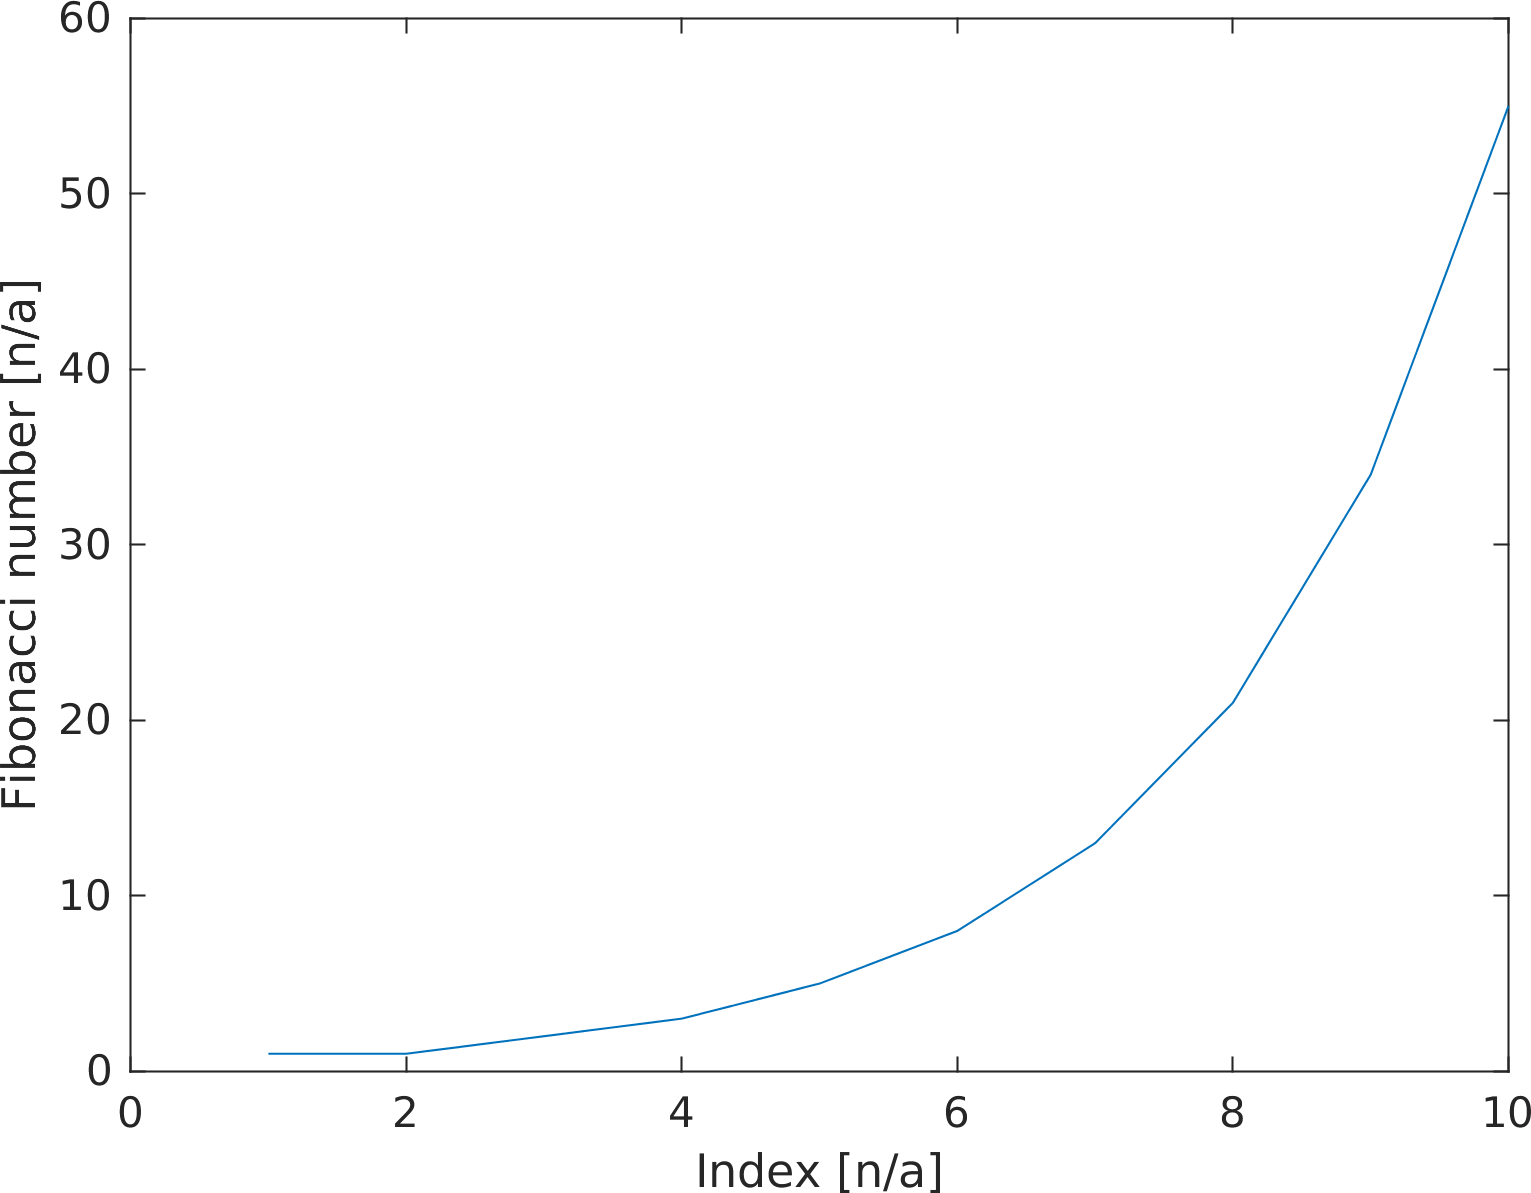
\includegraphics[scale=0.7]{images/figure04_fib}}
\caption{The first 10 elements of the Fibonacci sequence}
\label{fig:fibonacci}
\end{figure}

This way of looking at a vector is often useful for debugging, especially
if it is big enough that displaying the elements on
the screen is unwieldy.


\section{Common Vector Operations}

We've covered some basic features of vectors. Let's now look at some common patterns we use to work with data stored in vectors.

\subsection{Reduce}
\label{reduce}

We frequently use loops to run through the elements of a vector
and add them up, multiply them together, compute the sum
of their squares, and so on.  This kind of operation is called \emph{reduce},
because it reduces a vector with multiple elements down to a single
number.

\index{reduce}
\index{vector}

For example, the loop in Listing~\ref{lst:vec_reduce} adds up the elements of a vector named \lstinline{X} (which we assume has been defined).

\begin{lstlisting}[caption={Reducing a vector to a single scalar value (the sum)}, label={lst:vec_reduce}]
total = 0
for i=1:length(X)
    total = total + X(i)
end
ans = total
\end{lstlisting}

The use of \lstinline{total} as an accumulator is similar to what we
saw in Chapter~3.  Again, we use the \lstinline{length} function
to find the upper bound of the range, so this loop will work
regardless of the length of \lstinline{X}.
Each time through the loop, we add
in the \lstinline{i}th element of \lstinline{X}, so at the end of the loop
\lstinline{total} contains the sum of the elements.

\index{accumulator}
\index{length function@\lstinline{length} function}

MATLAB provides functions that perform some reduce operations.
For example, the \lstinline{sum} function computes the sum of the elements
in a vector, and \lstinline{prod} computes the product.


\subsection{Apply}
\label{apply}

Another common use of a loop is to run through the elements of
a vector, perform some operation on the elements, and create
a new vector with the results.  This operation is called
\emph{apply}, because you apply the operation to each element in
the vector.

\index{apply}

For example, the loop in Listing~\ref{lst:vec_apply} creates a vector \lstinline{Y} that
contains the squares of the elements of \lstinline{X} (assuming, again, that \lstinline{X} is already defined).

\begin{lstlisting}[caption={Making a new vector Y by squaring the elements in X}, label={lst:vec_apply}]
for i=1:length(X)
    Y(i) = X(i)^2
end
\end{lstlisting}

Many apply operations can be done with element-wise operators.
The following statement is more concise than the loop in
Listing~\ref{lst:vec_apply}.

\begin{code}
Y = X .^ 2
\end{code}

It also runs faster!


\section{Chapter Review}

In this chapter, we used a vector to store the elements of a sequence.  We learned how to select elements from a vector and perform vector arithmetic.  We performed reduce and apply operations using \lstinline{for} loops, MATLAB functions, and element-wise operations.

Here are some terms from this chapter you might want to remember.

% A {\em compound statement} is a statement, like \lstinline{if} and \lstinline{for}, that
% contains other statements in an indented body.
% If you put one compound statement in the body of another, they are {\em nested}.

% A {\em scalar} is single value; a
A \emph{vector} is a sequence of values, which is a kind of \emph{matrix}, also called an \emph{array} in some MATLAB documentation.

An \emph{index} is an integer value used to indicate one of the elements
in a vector or matrix (also called a \emph{subscript} in some MATLAB documentation).

An operation is \emph{element-wise} if it acts on the individual elements of a vector or matrix (unlike some linear algebra operations).

% You can {\em search} a vector for an element that has some desired property.
You can \emph{apply} an operation to all elements of a vector, and you can \mbox{\emph{reduce}} a vector to a single value, for example by computing the sum of the elements.

% A {\em name collision} is a scenario where two scripts that use the same variable name interfere with each other.

In the next chapter, we'll meet the most important idea in computer programming: functions!



\section{Exercises}

Before you go on, you might want to work on the following exercises.

\begin{ex}
(From \href{https://ocw.mit.edu/courses/18-s997-introduction-to-matlab-programming-fall-2011/pages/the-basics/lists-vectors-and-matrices/}{18.S997 OCW.})

Practice creating vectors in various ways.
\begin{itemize}
\item Try out sequences with step-size other than 1, e.g. \lstinline{[4:0.1:5], [5:-2:-5]}.
\item Create a list of the whole numbers between 10 and 20 (inclusive), find their sum.
\item Create the vector of the previous question in decreasing order.
\item Find the sum of the odd numbers between 100 and 200.
\end{itemize}
\end{ex}

\begin{ex}
Write a loop that computes the first $n$ elements
of the geometric sequence $A_{i+1} = A_i/2$ with $A_1 = 1$.  Notice that
math notation puts $A_{i+1}$ on the left side of the equality.
When you translate to MATLAB, you might want to rewrite it with
$A_{i}$ on the left side.
\end{ex}


\begin{ex}
Write an expression that computes the square root of the sum of the squares of the elements of a vector, without using a loop.
\end{ex}

\index{square root}


\begin{ex}
\label{fibratio}

The ratio of consecutive Fibonacci numbers, $F_{n+1}/F_{n}$, converges
to a constant value as $n$ increases.  Write a script that computes
a vector with the first $n$ elements of a Fibonacci sequence (assuming
that the variable \lstinline{n} is defined) and then computes a new
vector that contains the ratios of consecutive Fibonacci numbers.
Plot this vector to see if it seems to converge.  What value does
it converge on?

\index{Fibonacci}

% fibonacci4.m
\end{ex}


\begin{ex}
  The following set of equations is based on a famous example of a chaotic system, the Lorenz attractor (see \url{https://greenteapress.com/matlab/lorenz}):
%
\begin{eqnarray*}
x_{i+1} &=& x_i + \sigma \left( y_i - x_i \right) dt  \\
y_{i+1} &=& y_i + \left[ x_i (r - z_i) - y_i \right] dt   \\
z_{i+1} &=& z_i + \left( x_i y_i - b z_i \right) dt
\end{eqnarray*}
%
\begin{enumerate}

\item Write a script that computes the first 10 elements of the sequences
$X$, $Y$, and $Z$ and stores them in vectors named \textbf{\lstinline{X}}, \textbf{\lstinline{Y}},
and \textbf{\lstinline{Z}}.

Use the initial values $X_1 = 1$, $Y_1 = 2$, and $Z_1 = 3$ with the values
$\sigma = 10$, $b = 8/3$, $r = 28$, and $dt = 0.01$.

\item Read the documentation for \lstinline{plot3} and \lstinline{comet3}, and
plot the results in three dimensions.

\item Once the code is working, use semicolons to suppress the output
and then run the program with sequence lengths of 100, 1,000, and 10,000.

\item Run the program again with different starting conditions.
What effect does it have on the result?

\item Run the program with different values for $\sigma$, $b$, and $r$,
and see if you can get a sense of how each variable affects the
system.

\end{enumerate}

\index{Lorenz attractor}
% lorenz.m

\end{ex}


\begin{ex}
The logistic map (see \url{https://greenteapress.com/matlab/logistic}) is described by the following equation:

\index{logistic map}

\begin{equation*}
X_{i+1} = r X_i (1-X_i)
\end{equation*}
where $X_i$ is a number between 0 and 1, and $r$ is a positive number.

\begin{enumerate}

\item Write a script named \emph{logmap.m} that computes the first 50
elements of $X$ with \lstinline{r} = 3.9 and \lstinline{X1} = 0.5, where
\lstinline{r} is the parameter of the logistic map and \lstinline{X1} is the
initial value.

\item Plot the results for a range of values of $r$ from 2.4 to 4.0.
How does the behavior of the system change as you vary $r$?

\end{enumerate}

% logmap.m

\end{ex}

\clearpage

\begin{ex}

For this exercise write a live script named \emph{firstorder.mlx} to examine the connection between a geometric series (progression) and the time response of a first-order system.

A first-order, linear ordinary differential equation (ODE) is a common mathematical model useful to predict the behavior of many engineering systems.  A typical form for a system undergoing decay is
\begin{equation*}
     \frac{dy}{dt} = -k \, y(t)
\end{equation*}
where $y(t)$ is the quantity that decays over time, $k$ is the constant decay rate and $t$ is time.  The solution to this ODE is
\begin{equation*}
     y(t) = y_0 \, e^{-kt}
\end{equation*}
where $y_0$ is the initial condition.

Computers, and computer programs, don't have a way to handle such this continuous time function directly.  One thing we can do is to sample the function at discrete points and plot the results.

\begin{itemize}
     \item Write text block and code block to illustrate a specific example of the time response, $y(t)$, where $y_0 = 20$ units and $k=\SI{2}{s^{-1}}$.  Use the \lstinline{linspace} command to create a time vector of length 100, starting at 0 and ending at 4. Plot the first-order decay as $y(t)$ vs time.
\end{itemize}

In computational solutions, we often approximate continuous processes using discrete time steps because computers operate with finite, step-by-step calculations. They cannot directly handle continuous, infinitely varying data.  We can approximate the above ODE with the following \emph{difference equation}:
\begin{equation*}
     y[n] = y[n-1] (1- k \Delta t)
\end{equation*}
where $y[n]$ is the value at the $n$-th time step, $y[n-1]$ is the value at the previous time step and $\Delta t$ is the time step between consecutive points in the discrete-time system. This is the interval over which we are updating the system's state from one step to the next.

\begin{itemize}
     \item Add text and code plots to implement the recurrent, discrete time approximation.  Start with a small time step, say $\Delta t = \SI{0.04}{s}$ Plot the discrete time approximation on the same axes you used for the sampled analytical solution and use a discrete marker to show each element in the solution.
     \item Experiment with increasing the time step to see how it affects the approximation.  Add a text block to the live script to describe the effect of the time step on the accuracy of the discrete time approximation.
\end{itemize}

\end{ex}
\chapter{Functions}
\label{functions}


This chapter introduces the most important idea in computer programming: \mbox{functions}!
To explain why functions are so important, I'll start by explaining one of the problems they solve: name collisions.

\index{function}

\section{Name Collisions}
\label{collision}

\index{name collision}
\index{collision!name}
\index{workspace}

All scripts run in the same workspace, so if one script changes the value of a variable, all other scripts see the change.  With a few simple scripts, that's not a problem, but eventually the interactions between scripts become unmanageable.

For example, the following script computes the
sum of the first \lstinline{n} terms in a geometric sequence, but it also
has the {\em side effect} of assigning values to \lstinline{A1}, \lstinline{total},
\lstinline{i}, and \lstinline{a}.

\begin{code}
A1 = 1;
total = 0;
for i=1:10
    a = A1 * 0.5^(i-1);
    total = total + a;
end
ans = total
\end{code}

If you were using any of those variable names before calling this
script, you might be surprised to find, after running the script,
that their values had changed.  If you have two scripts that use
the same variable names, you might find that they work separately
and then break when you try to combine them.  This kind of
interaction is called a \emph{name collision}.

\index{script}

As the number of scripts you write increases, and they get longer
and more complex, name collisions become more of a problem.  One of the several motivations for functions is to avoid this problem by limiting the \emph{scope} of the variables within the function to be \emph{local} to that function.  This is one instance of \emph{encapsulation}, a common strategy to manage program complexity.  The function encapsulates the local variables so that they are only accessible within the function.


\section{Defining Functions}

A \emph{function} is like a script, except that each function has its own workspace, so any local variables defined
inside a function only exist while the function is running and don't
interfere with variables in other workspaces, even if they have the
same name.  In other words, the scope of the local variables within the function are limited to only the operations the function.
Function inputs and outputs are defined carefully to avoid
unexpected interactions.

To define a new function, you create an M-file with the name you
want and put a function definition in it.  For example, to create
a function named \lstinline{myfunc}, create an M-file named \emph{myfunc.m}
and put the following definition into it (Listing~\ref{lst:function_def}):

\index{M-file}
\index{script}
\index{function definition}

\begin{lstlisting}[caption={A function definition}, label={lst:function_def}]
function res = myfunc(x)
    s = sin(x)
    c = cos(x)
    res = abs(s) + abs(c)
end
\end{lstlisting}

The first non-comment word of the file has to be \lstinline{function}, because
that's how MATLAB tells the difference between a script and a function
file.

\index{compound statement}
\index{definition!function}

A function definition is a compound statement.  The first line
is called the \emph{signature} of the function; it defines
the inputs and outputs of the function.  In Listing~\ref{lst:function_def} the \emph{input variable} is named \lstinline{x}.  When this function is called, the
argument provided by the user will be assigned to \lstinline{x}.

\index{input variable}
\index{variable!input}

\index{output variable}
\index{variable!output}

The \emph{output variable} is named \lstinline{res}, which is short for
\emph{result}.  You can call the output variable whatever you want, but
as a convention, I like to call it \lstinline{res}.  Usually the last
thing a function does is assign a value to the output \mbox{variable}.

\index{res@\lstinline{res}}
\index{ans@\lstinline{ans}}

Once you've defined a new function, you call it the same way you
call built-in MATLAB functions.  If you call the function as a statement,
MATLAB puts the result into \lstinline{ans}:

\begin{code}
>> myfunc(1)

s = 0.84147098480790

c = 0.54030230586814

res = 1.38177329067604

ans = 1.38177329067604
\end{code}

But it's more common (and better style) to assign the result to
a variable:

\begin{code}
>> y = myfunc(1)

s = 0.84147098480790

c = 0.54030230586814

res = 1.38177329067604

y = 1.38177329067604
\end{code}

While you're debugging a new function, you might want to display
intermediate results like this, but once it's working, you'll want
to add semicolons to make it a \emph{silent function}.  A silent function
computes a result but doesn't display
anything (except sometimes warning messages). Most built-in
functions are silent.

\index{silent function}
\index{function!silent}
\index{workspace}

Each function has its own workspace, which is created when the
function starts and destroyed when the function ends.  If you try to
access (read or write) the variables defined inside a function, you
will find that they don't exist.

\begin{code}
>> clear
>> y = myfunc(1);
>> who
Your variables are: y

>> s
Undefined function or variable 's'.
\end{code}

The only value from the function that you can access is the result,
which in this case is assigned to \lstinline{y}.

If you have variables named \lstinline{s} or \lstinline{c} in your workspace
before you call \lstinline{myfunc}, they will still be there when the
function completes.

\begin{code}
>> s = 1;
>> c = 1;
>> y = myfunc(1);
>> s, c

s = 1
c = 1
\end{code}

So inside a function you can use whatever variable names you
want without worrying about collisions.

\index{name collision}
\index{collision!name}


\section{Function Documentation}

% \index{documentation}
\index{comment}

At the beginning of every function file, you should include a comment that explains what the function does:

\index{documentation!function}

\begin{code}
    function res = myfunc(x)
    %MYFUNC Manhattan distance from the origin to a point on the unit circle.
    %   d = MYFUNC(d) is the distance from the origin to a point on the unit
    %   circle with (x) as the angle in radians.
    
        s = sin(x);
        c = cos(x);
        res = abs(s) + abs(c);
    
    end
\end{code}

When you ask for \lstinline{help}, MATLAB prints the comment you provide.

\index{help@\lstinline{help}}

% Emulate the way MATLAB prints CAPS into bold.
\begin{lstlisting}[language=C, keywordstyle=\bfseries, morekeywords={myfunc}]
    >> help myfunc
    myfunc Manhattan distance from the origin to a point on the unit circle.
       d = myfunc(d) is the distance from the origin to a point on the unit
       circle with (x) as the angle in radians.
\end{lstlisting}

There are lots of conventions about what should be included
in these comments.  Looking at examples of documentation for MATLAB's included functions can be a productive way to understand the style and convention used in documenting functions.  You can open code a MATLAB function in and Editor window (read-only) to better see the raw text.  For example,
\begin{code}
    >> edit mean
\end{code}
will open the \emph{mean.m} function file.


Among other things, it's a good idea to
include the following:

\begin{description}

\item [Signature] The signature of the function, which includes the name
of the function, the input variable(s), and the output variable(s).

\item [Description] A clear, concise, abstract description of what the function does.
An \emph{abstract} description is one that leaves out the
details of \emph{how} the function works and includes only information
that someone  using the function needs to know.  You can put additional
comments inside the function that explain the details.

\item [Variables] An explanation of what the input and output variables mean; for example,
in this case it is important to note that \lstinline{x} is considered
to be an angle in radians.

\item [Examples] Working examples of how you would use the function.  Often functions can be called in different ways, so providing examples of the applicable use cases helps convey the intended implementations.

\item [See Also] If there are related functions, listing them can be really helpful for future users, including yourself.  For example the \lstinline{mean} function lists \lstinline{median, median, std, min, max, var, cov, mode}---all related reduce operations that produce summary statistics.

\end{description}

\index{precondition}
\index{postcondition}

\section{Naming Functions}
%\index{Functions!naming}

There are a few ``gotchas'' that come up when you start defining functions.
The first is that the ``real'' name of your function is determined by the file name, \emph{not} by the name you put in the function signature.  As a matter of style, you
should make sure that they are always the same, but if you
make a mistake, or if you change the name of a function, it's
easy to get confused.

\index{function name}
\index{name!function}

In the spirit of making errors on purpose, edit \emph{myfunc.m} and change the name of the function from \textbf{\lstinline{myfunc}} to \textbf{\lstinline{something_else}}, like this:

\begin{code}
function res = something_else (x)
    s = sin(x);
    c = cos(x);
    res = abs(s) + abs(c);
end
\end{code}

Now call the function from the Command Window, like this:

\begin{code}
>> y = myfunc(1)
y = 1.3818
\end{code}

The function is still called \lstinline{myfunc}, because that's the name of the file.
If you try to call it like this:

\begin{code}
>> y = something_else(1)
Undefined function or variable 'something_else'.
\end{code}

It doesn't work.  The name of the file is what matters; the name of the function is ignored.

The second ``gotcha'' is that the name of the file can't have spaces.
For example, if you rename the file to \emph{my func.m}
and try to run it, you get:

\begin{code}
>> y = my func(1)
 y = my func(1)
        |
Error: Unexpected MATLAB expression.
\end{code}

This fails because MATLAB thinks \lstinline{my} and \lstinline{func} are two different
variable names.

The third ``gotcha'' is that your function names can collide with built-in
MATLAB functions.  For example, if you create an M-file named \emph{sum.m} and then call \lstinline{sum}, MATLAB might call your new
function, not the built-in version!  Which one actually gets called
depends on the order of the directories in the search path and
(in some cases) on the arguments.  As an example, put the following
code in a file named \emph{sum.m}:

\index{name collision}
\index{collision!name}

\begin{code}
function res = sum(x)
   res = 7;
end
\end{code}

And then try this:

\begin{code}
>> sum(1:3)

ans = 6

>> sum

ans = 7
\end{code}

In the first case MATLAB used the built-in function; in the second
case it ran your function!  This kind of interaction can be very
confusing.  Before you create a new function, check to see if there is
already a MATLAB function with the same name.  If there is, choose
another name!

\section{Multiple Input Variables}
\label{hypotenuse}

\index{input variable}
\index{variable!input}

Functions can take more than one input variable.
For example, the following function in Listing~\ref{lst:hyp_function} takes two input variables,
\lstinline{a} and \lstinline{b}:

\begin{lstlisting}[caption={A function that computes the sum of squares of two numbers}, label={lst:hyp_function}]
function res = sum_squares(a, b)
    res = a^2 + b^2;
end
\end{lstlisting}

This function computes the sum of squares of two numbers, \lstinline{a}
and \lstinline{b}.

If we call it from the Command Window with arguments 3 and 4, we can
confirm that the sum of their squares is 25.

\begin{code}
>> ss = sum_squares(3, 4)
ss = 25
\end{code}

The arguments you provide are assigned to the input variables in
order, so in this case 3 is assigned to \lstinline{a} and 4 is assigned to
\lstinline{b}.  MATLAB checks that you provide the right number of arguments;
if you provide too few, you get

\begin{code}
>> ss = sum_squares(3)
Not enough input arguments.

Error in sum_squares (line 4)
    res = a^2 + b^2;
\end{code}

This error message might be confusing, because it suggests that
the problem is in \lstinline{sum_squares} rather than in the function call.
Keep that in mind when you're debugging.

If you provide too many arguments, you get

\begin{code}
ss = sum_squares(3, 4, 5)
Error using sum_squares
Too many input arguments.
\end{code}

That's a better error message, because it's clear that the problem isn't in the function, it's in the way we're using the function.

\section{Multiple Output Variables}

Functions can also return multiple output variables.  Here is an example of a function that returns two variables:
\begin{code}
function [s, p] = sum_and_product(a, b) 
    s = a + b;
    p = a * b;
\end{code}

We can call this function and assign the output to variables in the workspace, making sure to include the square brackets, like this:
\begin{code}
    >> [added, multiplied] = sum_and_product(4, 5)
    added =
         9
    multiplied =
        20
\end{code}

There are some potential gotchas here as well.  If we only provide one output in the function call, MATLAB will return just the first output variable without a warning or error:
\begin{code}
    >> added = sum_and_product(4, 5)
    added =
         9    
\end{code}
Also, if we don't include the square brackets, both variables will be assigned the first output, which is probably not what we would intend:
\begin{code}
    >> added, multiplied = sum_and_product(4, 5)
    added =
         9
    multiplied =
         9
\end{code}

\section{Local Functions}
The primary way to create a MATLAB function is to have a single function in a single m-file where the function and the file share the same name.  An alternative is to have a function within a script or to have multiple functions within the same m-file, called a \emph{local function}.   This can be helpful if you don't want to create an manage many separate files. These local functions are only accessible from file in which they are defined; they can't be accessed directly from the command line.

For example, we could create a scipt named \Verb[fontshape=it]|local_function_demo.m|
with the following code:

\begin{code}
    function y = my_local_func(x)
    % Local function to compute the square of x.
    y = x^2;
    end
    
    % Call the local function
    b = my_local_func(2)    
\end{code}

Then we can run the script from the command window:
\begin{code}
    >> local_function_demo
    b =
         4
\end{code}
which works as expected.  You might also notice that you can't call the \lstinline{my_local_func} directly from the command window, because it is local to the script:
\begin{code}
    >> my_local_function(3)
    Unrecognized function or variable 'my_local_function'. 
\end{code}

This behavior is particularly useful when using live scripts so that you can have various functions and the code that calls them all in the same live script document.

Note: Before R2024a, local functions in scripts must be defined at the end of the file, after the last line of script code.

\section{Chapter Review}

Now that we know about functions, and all the ways they can go wrong, let's put them to good use.  In the next chapter we'll develop a program that uses several functions to search for Pythagorean triples (and I'll explain what those are).

Here are a few terms in this chapter you might want to remember.

A \emph{function} is a named sequence of statements stored in an M-file.
A function can have one or more \emph{input variables}, which get their values when the function is called, and \emph{output variables}, which return a value from the function to the caller.

The first line of a function definition is its \emph{signature}, which
specifies the name of the function, the input variables, and the
output variables.

A \emph{silent function} doesn't display anything, generate a figure, or have any other effect other than returning output values.


\section{Exercise}

Before you go on, you might want to work on the following exercise.

\begin{ex}
\label{hypotenuse_exercise}
Write a function called \textbf{\lstinline{hypotenuse}} that takes two parameters, \textbf{\lstinline{a}} and \textbf{\lstinline{b}}, that represent the lengths of two sides of a right triangle.  It should assign to \lstinline{res} the length of the third side of the triangle, given by the formula

\[ c = \sqrt{a^2 + b^2} \]

\end{ex}

\chapter{Conditionals}


In this chapter, we'll use functions and a new feature---conditional statements---to search for Pythagorean triples.
A Pytha\-gorean triple is a set of integers, like~3, 4, and 5,
that are the lengths of the sides of a right triangle.  Mathematically, it's a set of integers $a$, $b$, and $c$ such that $a^2 + b^2 = c^2$.
This example will also demonstrate the \emph{incremental development} process we talked about in Chapter~\ref{loops}.

\index{Pythagorean triple}

\section{Relational Operators}
\index{operator!relational}

Suppose we have three variables, \lstinline{a}, \lstinline{b}, and \lstinline{c}, and we want to check whether they form a Pythagorean triple.  We can use the equality operator (\lstinline{==}) to compare two values:

\begin{code}
>> a = 3;
>> b = 4;
>> c = 5;
>> a^2 + b^2 == c^2

ans = logical 1
\end{code}

The result is a \emph{logical} data type, which means it's either~\lstinline{1}, which means ``true,'' or~\lstinline{0}, which means ``false.''  In fact, you can use \lstinline{true} as substitute for \lstinline{1} and \lstinline{false} as shorthand for \lstinline{0}:
\begin{code}
    >> true
    ans =
      logical
       1
    >> true == 1
    ans =
      logical
       1
\end{code}


Here's an example where the result is false:

\begin{code}
>> c = 6;
>> a^2 + b^2 == c^2
ans = logical 0
\end{code}

It's a common error to use the assignment operator (\lstinline{=}) instead of the equality operator (\lstinline{==}).  If you do, you get an error:

\begin{code}
>> a^2 + b^2 = c^2
 a^2 + b^2 = c^2
           |
Error: Incorrect use of '=' operator.
To assign a value to a variable, use '='.
To compare values for equality, use '=='.
\end{code}

The equality operator is one of several \emph{relational operators}, so called because they test relations between values.
For example, \lstinline{x < 10} is true (\lstinline{1}) if the value of \lstinline{x} is less than \lstinline{10} or false (\lstinline{0}) if otherwise.  And \lstinline{x > 0} is true if \lstinline{x} is greater than~\lstinline{0}.

The other relational operators are \lstinline{<=} for ``less or equal,'' \lstinline{>=} for ``greater or equal,'' and  \lstinline{~=} for ``not equal.''


\section{if Statement}

\index{if statement@\lstinline{if} statement}
\index{conditional statement}

Now suppose that when we find a Pythagorean triple we want to display a message.
The \lstinline{if} statement allows you to check for certain conditions
and execute statements if the conditions are met.  For example:

\begin{code}
if a^2 + b^2 == c^2
    disp("Yes, that is a Pythagorean triple.")
end
\end{code}

The syntax is similar to a \lstinline{for} loop.  The first line
specifies the condition we're interested in.  If the condition is true,
MATLAB executes the \emph{body} of the statement, which is the indented sequence of
statements between the \lstinline{if} and the \lstinline{end}.

\index{indentation}

MATLAB doesn't require you to indent the body of an \lstinline{if}
statement, but it makes your code more readable, so you should do it.

If the condition is not satisfied, the statements in the body are
not \mbox{executed}.

Sometimes there are alternative statements to
execute when the condition is false.  In that case, you can extend
the \lstinline{if} statement with an \lstinline{else} clause.

\index{else clause@\lstinline{else} clause}

The complete version of the previous example might look like this:

\begin{code}
if a^2 + b^2 == c^2
    disp("Yes, that is a Pythagorean triple.")
else
    disp("No, that is not a Pythagorean triple.")
end
\end{code}

Statements like \lstinline{if} and \lstinline{for} that contain other statements
are called \emph{compound} statements.  All compound statements finish
with \lstinline{end}.

\index{compound statement}
\index{statement!compound}



\section{Incremental Development}
\label{increxample}
\index{incremental development}

Now that we have relational operators and \lstinline{if} statements, let's start writing
the program.

Here are the steps we will follow to develop the program incrementally:

\begin{enumerate}

\item Write a script named \emph{find\_triples.m} and start with a loop that enumerates values of \lstinline{a} and displays them.

\item Write a second loop that enumerates values of \lstinline{b} and a third loop that enumerates values of \lstinline{c}.

\item Use the if statement from the previous section to check whether \lstinline{a}, \lstinline{b}, and \lstinline{c} form a Pythagorean triple.

\item Display the values that pass the test.

\item Transform the script into a function and make it take an input variable that specifies the range to search.

\end{enumerate}

Along the way, we'll optimize the program to eliminate unnecessary work.


\section{Logical Functions}

The first step is to create a \emph{logical function}, which is a function that returns a logical value.
The following function takes three input variables, \lstinline{a}, \lstinline{b}, and~\lstinline{c}, and returns true (\lstinline{1}) if they form a Pythagorean triple and false (\lstinline{0}) otherwise.

\begin{code}
function res = is_pythagorean(a, b, c)
    if a^2 + b^2 == c^2
        res = 1;
    else
        res = 0;
    end
end
\end{code}

We can use this function like so:


\begin{code}
>> is_pythagorean(3, 4, 5)
ans = 1
\end{code}

But we can write the same function more concisely, like this:

\begin{code}
function res = is_pythagorean(a, b, c)
    res = a^2 + b^2 == c^2;
end
\end{code}

The result of the equality operator is a logical value, which we can assign directly
to \lstinline{res}.

Put this function in a file called \emph{is\_pythagorean.m}, so we can use it as part of our program.


\section{Nested Loops}

The next step is to write loops that enumerate different values of \lstinline{a}, \lstinline{b}, and
\lstinline{c}.  Create a new file called \emph{find\_triples.m} where we'll develop the rest of the program.

\index{nested loop}
\index{loop!nested}

We'll start with a loop for \lstinline{a}:

\begin{code}
for a=1:3
    a
end
\end{code}

It might seem silly to start with such a simple program, but this is an essential element of incremental development: start simple and test as you go.

The output is as expected.

\begin{code}
1
2
3
\end{code}

Now we'll add a second loop for \lstinline{b}.  It might be tempting to write something like this:

\begin{code}
for a=1:3
    disp(a)
end
for b=1:4
    disp(b)
end
\end{code}

But that loops through the values of \lstinline{a} and then loops through the values of \lstinline{b}, and that's not what we want.

Instead, we want to consider every possible pair of values, like this:

\begin{code}
for a=1:3
    for b=1:4
        disp([a,b])
    end
end
\end{code}

Now one loop is inside the other.  The inner loop gets executed three times, once for each value of \lstinline{a}, so here's what the output looks like (I've adjusted the spacing to make the structure clear):

\begin{code}
>> find_triples
     1     1
     1     2
     1     3
     1     4
     2     1
     2     2
     2     3
     2     4
     3     1
     3     2
     3     3
     3     4
\end{code}

The left column shows the values of \lstinline{a} and the right column shows the values of \lstinline{b}.

The next step is to search for values of \lstinline{c} that might make a Pythagorean triple.  The largest possible value for \lstinline{c} is \lstinline{a + b}, because otherwise we couldn't form a triangle
(see \url{https://greenteapress.com/matlab/triangle}).

\begin{code}
for a=1:3
    for b=1:4
        for c=1:a+b
            disp([a,b,c])
        end
    end
end
\end{code}

After each small change, run the program again and check the output.

\section{Putting It Together}

Now instead of displaying all of the triples, we'll add an \lstinline{if} statement and display only Pythagorean triples:

\begin{code}
for a=1:3
    for b=1:4
        for c=1:a+b
            if is_pythagorean(a, b, c)
                disp([a,b,c])
            end
        end
    end
end
\end{code}

The result is just one triple:

\begin{code}
>> find_triples
     3     4     5
\end{code}

You might notice that we're wasting some effort here.
After checking the case when \lstinline{a} is~1 and \lstinline{b} is~2, there's no point in checking
the case when \lstinline{a} is~2 and \lstinline{b} is~1.  We can save the extra work by adjusting the
range of \lstinline{b}:

\begin{code}
for b=a:4
\end{code}

We can save even more work by adjusting the range of \lstinline{c}:

\begin{code}
for c=b:a+b
\end{code}

Here's the final version:

\begin{code}
for a=1:3
    for b=a:4
        for c=b:a+b
            if is_pythagorean(a, b, c)
                disp([a,b,c])
            end
        end
    end
end
\end{code}

\section{Encapsulation and Generalization}

As a script, this program has the side effect of assigning values to
\lstinline{a}, \lstinline{b}, and \lstinline{c}, which would be bad if any of those names were in use.
By wrapping the code in a function, we can avoid name collisions; this process is called \emph{encapsulation} because it isolates this program from the workspace.

\index{encapsulation}
\index{generalization}

The first draft of the function takes no input variables:

\begin{code}
function res = find_triples()
    for a=1:3
        for b=a:4
            for c=b:a+b
                if is_pythagorean(a, b, c)
                    disp([a,b,c])
                end
            end
        end
    end
end
\end{code}

The empty parentheses in the signature are not necessary, but
they make it apparent that there are no input variables.  Similarly,
it's a good  idea when calling the new function to use parentheses as a reminder
that it's a function, not a script:

\begin{code}
>> find_triples()
\end{code}

The output variable isn't necessary, either; it
never gets assigned a value.  But I put it there as a matter of
habit and so my function signatures all have the same structure.

\index{output variable}
\index{variable!output}

The next step is to generalize this function by adding input
variables.  The natural generalization is to replace the constant
values~\lstinline{3} and~\lstinline{4} with a variable, so we can search an arbitrarily large
range of values.

\begin{code}
function res = find_triples(n)
    for a=1:n
        for b=a:n
            for c=b:a+b
                if is_pythagorean(a, b, c)
                    disp([a,b,c])
                end
            end
        end
    end
end
\end{code}

Here are the results for the range from 1 to 15:

\begin{code}
>> find_triples(15)
     3     4     5
     5    12    13
     6     8    10
     8    15    17
     9    12    15
\end{code}

The triples $5,12,13$ and $8,15,17$ are new, but the others are just multiples of the $3,4,5$ triangle.

\section{Adding a continue Statement}

\index{continue@\lstinline{continue}}

As a final improvement, let's modify the function so it only
displays the ``lowest'' of each Pythagorean triple, and not the
multiples.

The simplest way to eliminate the multiples is to check whether
\lstinline{a} and \lstinline{b} share a common factor.  If they do, dividing both
by the common factor yields a smaller, similar triangle that has
already been checked.

\index{gcd function@\lstinline{gcd} function}
\index{function!gcd@\lstinline{gcd}}

MATLAB provides a \lstinline{gcd} function that computes the greatest common
divisor of two numbers.  If \lstinline{gcd(a,b)} is greater than 1,
\lstinline{a} and \lstinline{b} share a common factor, and we can use the \lstinline{continue}
statement to skip to the next pair. Listing~\ref{lst:triples_function} contains the final version of this function:

\begin{lstlisting}[caption={Our final Pythagorean triples function}, label={lst:triples_function}]
function res = find_triples(n)
    for a=1:n
        for b=a:n
            for c=b:a+b
                if gcd(a,b) > 1
	                continue
                end
                if is_pythagorean(a, b, c)
                    disp([a,b,c])
                end
            end
        end
    end
end
\end{lstlisting}

The \lstinline{continue} statement  causes the program to end the current iteration
immediately, jump to the top of the loop, and ``continue'' with the next iteration.

In this case, since there are three loops, it might not be obvious which loop to jump to, but the rule is to jump to the innermost loop (which is what we want).

Here are the results with \lstinline{n = 40}:

\begin{code}
>> find_triples(40)
     3     4     5
     5    12    13
     7    24    25
     8    15    17
     9    40    41
    12    35    37
    20    21    29
\end{code}


\section{How Functions Work}
\index{function}

Let's review the sequence of steps that occur when you call a function:

\begin{enumerate}

\item Before the function starts running, MATLAB creates a new
workspace for it.
\index{workspace}

\item MATLAB evaluates each of the arguments and assigns
the resulting values, in order, to the input variables (which
live in the \emph{new} workspace).

\item The body of the code executes.  Somewhere in the body
a value gets assigned to the output variable(s).

\item The function's workspace is destroyed; the only thing
that remains is the value of the output variable(s) and any side
effects the function had (like displaying values).

\item The program resumes from where it left off.  The value(s)
of the function call is the value(s) of the output variable(s).

\end{enumerate}

When you're reading a program, and you come to a function call,
there are two ways to interpret it. You can think about the mechanism I just described,
and follow the execution of the program into the function and back, or you can assume that the function works correctly, and go on to the next statement after the function call.

When you use a built-in function, it's natural to assume that it works, in part because you don't
usually have access to the code in the body of the function.
But when you start writing your own functions, you might
find yourself following the ``flow of execution.''  This can
be useful while you are learning, but as you gain experience, you
should get more comfortable with the idea of writing a function,
testing it to make sure it works, and then forgetting about the
details of how it works.

\index{flow of execution}
\index{abstraction}

Forgetting about details is called \emph{abstraction}; in the context
of functions, abstraction means forgetting about \emph{how} a function
works and just assuming (after appropriate testing) that it works.
For many people, it takes some time to get comfortable with functions.  If you are one of them, you might be tempted to avoid functions, and sometimes you can get by without them.

But experienced programmers use functions extensively, for several good reasons. First, each function has its own workspace, so using functions helps
avoid name collisions.
Functions also lend themselves to incremental development: you can
debug the body of the function first (as a script), then encapsulate
it as a function, and then generalize it by adding input variables.

Also, functions allow you to divide a large problem into small
pieces, work on the pieces one at a time, and then assemble a
complete solution.

Once you have a function working, you can forget about the
details of how it works and concentrate on what it does.  This
process of abstraction is an important tool for managing the
complexity of large programs.


\section{Chapter Review}

In this chapter, we encountered relational operators and \lstinline{if} statements, and we used them to develop a program that searches for Pythagorean triples.
We wrote a \emph{logical function}, which is a function that returns a logical value
(\lstinline{1} for ``true'' or \lstinline{0}~for ``false'').

We also saw an example of \emph{incremental development}, or developing programs gradually, adding just a few lines of code at a time and testing as you go.  If you develop programs this way, you will have fewer bugs, and you will find them more quickly.

This chapter defined two new terms: \emph{encapsulation} is the process of wrapping part of a program in
a function in order to limit interactions (including name collisions)
between the function and the rest of the program; \emph{abstraction} is the process of ignoring the details of how a function works in order to focus on a simpler model of what the
function does.

The next chapter introduces a new tool, called \lstinline{fzero}, that we'll use to solve nonlinear equations.


\section{Exercise}

Before you go on, you might want to work on the following exercise.

\begin{ex}
\index{Fibonacci number}
\index{Pythagorean triple}

There is an interesting connection between Fibonacci numbers and
Pythagorean triples.  If $F$ is a Fibonacci sequence, then

\begin{equation*}
\big(F_i F_{i+3}, \, 2 F_{i+1} F_{i+2}, \, F_{i+1}^2 + F_{i+2}^2 \big)
\end{equation*}
is a Pythagorean triple, for all $i \ge 1$.

Write a function named \lstinline{fib_triple} that
takes \lstinline{n} as an input variable, computes
the first \lstinline{n} Fibonacci numbers, stores them in a vector,
and checks whether this formula produces Pythagorean triples for numbers in the \mbox{sequence}.

% fib_triple.m

\end{ex}

\chapter{Data Types}
\label{c:datatypes}


In programming, we work with different kinds of information, or data. A \emph{data type} is a way of classifying this information, typically stored as a variable, so that the computer knows how to handle it. Just as different objects in everyday life serve different purposes, various kinds of data are handled differently in a program. For instance, numbers are often used in calculations, while text is treated as characters or words.

Think of data types like containers in your kitchen. If you want to store soup, you’d use a bowl, while juice would go in a glass. Similarly, in programming, you need to choose the right data type to store and process the information correctly. Using the right "container" helps ensure that the computer knows what to do with your data.

In MATLAB, understanding data types is essential not just for organizing your data, but also for interacting with the built-in tools and functions MATLAB offers. These tools use a variety of data types as both input and output. By knowing how to work with different data types, you can ensure that your programs communicate effectively with MATLAB’s powerful built-in functionality.

In this chapter, we'll explore most of the different data types in MATLAB, when to use them, and how this knowledge will help you interface better with MATLAB's capabilities.

\section{Numbers}

MATLAB, short for "matrix laboratory," was designed specifically for working with matrices, arrays, and vectors. In MATLAB, the fundamental data type for handling numerical values is the \emph{array}. This means that even single numbers (scalars), vectors, and matrices are all represented as arrays. We can even have empty arrays.  Understanding how MATLAB defines and uses these different types of arrays is essential to working efficiently with the software.

Here’s how MATLAB classifies these key terms:

\begin{description}
\item[Scalar:] An array with a single element.
\item[Vector:] A two-dimensional array that has either 1-by-N (a row vector) or N-by-1 (a column vector) dimensions.
\item[Matrix:] A two-dimensional array with more than one element in both dimensions.
\item[Array:] A general term in MATLAB that can refer to data with more than two dimensions.
\end{description}

By treating everything as an array, MATLAB simplifies many operations, making it easy to apply the same functions to scalars, vectors, matrices, and higher-dimensional arrays. 

The default type of number in a numeric array  \emph{double}, short for double-precision floating-point, and is suitable for most calculations due to its high precision and wide range. When you enter a number in MATLAB, it is automatically stored as a double, allowing for efficient handling of both integers and real numbers, including very large or very small values.

However, other numeric data types are important to understand, especially when interfacing with MATLAB utilities and libraries that expect specific types of input or output:

\begin{itemize}
    \item \textbf{Integers} (e.g., \texttt{int8}, \texttt{int16}, \texttt{int32}, \texttt{int64}): These types store whole numbers and are more memory-efficient when decimal values aren’t needed. For example, when counting items or processing digital signals, integers can save memory and improve performance.

    \item \textbf{Unsigned Integers} (e.g., \texttt{uint8}, \texttt{uint16}): These represent non-negative whole numbers and are commonly used in tasks such as image processing, where pixel values are naturally non-negative and often fall within a specific range (e.g., 0 to 255 for \texttt{uint8}).
\end{itemize}

You may encounter two special numeric values: \texttt{NaN} and \texttt{Inf}. These values arise in situations where the result of a calculation doesn’t produce a standard number and can be indicators of a bug.

\begin{itemize}
    \item \textbf{\texttt{NaN} (Not a Number):} This value represents undefined or unrepresentable results, such as the outcome of \texttt{0/0} or the square root of a negative number. \texttt{NaN} acts as a placeholder for invalid or missing numerical data and can propagate through calculations, indicating that the result is indeterminate.

    \item \textbf{\texttt{Inf} (Infinity):} This value occurs when a calculation produces a result too large to represent, such as division by zero (e.g., \texttt{1/0}). MATLAB distinguishes between positive (\texttt{Inf}) and negative infinity (\texttt{-Inf}). These values are often encountered in cases where numerical limits are exceeded, such as in iterative processes or extremely large datasets.
\end{itemize}

\section{Strings}

Under the hood, computer programs work with numbers, but people are often better at processing language.  To bridge this gap MATLAB uses arrays of \emph{characters} and arrays of \emph{strings}.

A character array is a one-dimensional sequence where each element is a \lstinline{char} type, analogous to the vectors we saw in Chapter~\ref{vectors} where each element was a number.   We can create a character array using a single quote, \lstinline{'}, and use some of the same techniques to determine the size and access elements via indexing.

\begin{code}
    charray = 'The quick brown fox';
    size(charray)
    ans =
         1    19
    charray(5:9)
    ans =
        'quick'
    charray(end-3:end)
    ans =
        ' fox'
\end{code}   

MATLAB uses a standard encoding to represent each character as a number (actually a 16-bit unsigned integer).  We can peer under the hood by converting the array of charters to an array of the codes:
\begin{code}
charray = 'hello!';
double(charray)
ans =
   104   101   108   108   111    33
\end{code}

A \lstinline{string} is a more powerful data type for storing text that simplifies manipulating text using functions such as \lstinline{contains}, \lstinline{replace} and \lstinline{split}.  You can create a string using double quotes, \lstinline{"}.  Strings, like numbers in MATLAB, are stored in arrays, so a single string is actually a 1-by-1 array of strings.

\begin{code}
str = "jumps over the lazy dog";
size(str)
ans =
     1     1
\end{code}
Because a string element is a single object, we can't use the same numerical indexing syntax, but MATLAB includes a function to support access by location:
\begin{code}
extractBetween(str, 16, 19)
ans = 
    "lazy"
\end{code}
We can use addition to concatenate strings, but there is no sense of subtraction
\begin{code}
hw = "hello" + " world!"
hw = 
    "hello world!"

h_w = "hello" - " world!"
Operator '-' is not supported for operands of type 'string'.
Error in types_examples (line 19)
h_w = "hello" - " world!"
\end{code}


\subsection{Creating Strings}

So far our examples have typically generated output to the Command Window in raw form.  We'll run into many situations where we'd like to improve the formatting of that text output, mixing numbers and letters.  This is particularly helpful when recording/logging data to a text file.

Two commands generate formatted strings: \lstinline{sprintf} which returns a formatted string 
and \lstinline{fprintf} which writes that string to the screen or a file.  For both commands we provide a \emph{format string} which contains the instructions for how to present the output.  Within the format string we can include \emph{special characters} that can't be included as ordinary text special two-character codes such as \lstinline{\n} for a new line and \lstinline{\t} for a tab.

\begin{code}
>> table_str = sprintf(" cats \t dogs \n salt \t pepper")
table_str = 
    " cats 	 dogs 
      salt 	 pepper"

>> disp(table_str);
 cats 	 dogs 
 salt 	 pepper

>> fprintf(" yin \t yang \n fish \t chips \n")
 yin 	 yang 
 fish 	 chips 
\end{code}

The format string can also include \emph{format specifiers} which are then replaced by numbers or characters in the specified format.  Format specifiers start with a percent sign, \lstinline{%}, and follow this prototype:
\begin{stdout}
%[identifier][flags][width][.precision][subtype]specifier
\end{stdout}   
The items within brackets are optional.  The \emph{specifier} indicates the format of the provided data.  Common specifiers are \lstinline{%f} for fixed point numbers, \lstinline{%d} for integers, \lstinline{%E} for exponential (scientific) notation and \lstinline{%s} for strings.

\begin{code}
>> % Fixed-point 
>> fprintf("pi = %f\n", pi);
pi = 3.141593
\end{code}
Notice that we added a newline character at the end of the format string, otherwise the next command prompt is on the same line as the output.

We can be more explicit by adding \emph{width} and \emph{precision} items to our format specifier:
\begin{code}
>> fprintf("pi also equals %4.2f\n", pi)
    pi also equals 3.14
\end{code}

We can provide multiple specifiers and values, which MATLAB uses in order:
\begin{code}
>> fprintf("There are %d %s and %d %s\n", ...
3, "apples", 5, "oranges");
    There are 3 apples and 5 oranges
\end{code}

And we can provide the arrays as values:
\begin{code}
>> fprintf("Random numbers: %5.3f\n", rand(1,3))
Random numbers: 0.766
Random numbers: 0.795
Random numbers: 0.187
>> fprintf("Random numbers: %5.3f, %5.3E, %.3f \n", rand(1,3))
Random numbers: 0.490, 4.456E-01, 0.646 
\end{code}

% ToDo - add \lstinline{append} and \lstinline{join}



\subsection{Analyzing Strings}

MATLAB also includes a number of ways to examine strings and take them apart.  These can be helpful for enabling MATLAB to process human-readable text or log files.  In this section we'll introduce a few of the common operations.

The \lstinline{strfind} function searches for a pattern.  The first argument is the string to be searched and the second is the pattern.  It returns an array of indexes where it found the pattern. The pattern can be another string:
\begin{code}
>> word = "Banana";
>> indexes = strfind(word, "a")
    indexes =
         2     4     6
>> indexes = strfind(word, "na")
    indexes =
          3     5
\end{code}
A similar function is \lstinline{contains} which uses the same syntax, but returns a logical scalar if the pattern is found.
\begin{code}
>> found = contains(word, "a")
found =
  logical
   1
>> found = contains(word, "b")
found =
  logical
   0
>> found = contains(word, "b", "IgnoreCase",true)
found =
  logical
   1
\end{code}

The \lstinline{split} function breaks a string into an array of strings based on a \emph{delimiter}, a character or sequence of characters that separates multiple elements in the same string.  Commas and backslashes are common delimiters in text data.  GPS receives can report their information with standard NMEA text sentences that are comma delimited.  

\begin{code}
>> gpsheading = "$HCHDG,123.4,0.0,E,5.5,W*3C";
>> parts = split(gpsheading, ",")
parts = 
  6x1 string array
    "$HCHDG"
    "123.4"
    "0.0"
    "E"
    "5.5"
    "W*3C"
\end{code}

We often want to convert these strings back into numerical values.  For strings that are only numbers, the \lstinline{str2num} function performs this operation.   If the string can't be interpreted as a number the function returns and empty array.  Continuing the GPS example above...
\begin{code}
>> hdg = str2num(parts(2))
    hdg =
      123.4000
>> direction = str2num(parts(4))
    direction =
         [] 
\end{code}

\section{Cell Arrays}

So far we've seen arrays of numbers and arrays of strings.  A cell array is a flexible data type where each element/cell can contain any type of data.
\begin{code}
    stra = ["hello", "world"];
vec = 5:-1:3;
num = 3.14;
carray = {stra, vec, num}
carray =
  1x3 cell array
    {["hello"    "world"]}    {[5 4 3]}    {[3.1400]}
\end{code}

The elements, or cells, are accessible by index, as with other MATLAB arrays, but in for cell arrays we use the curly braces \lstinline|{}|.  It is a little tricky when using an array of indexes to access multiple elements at one time.
\begin{code}
    a = carray{1}
    a = 
      1x2 string array
        "hello"    "world"
    [b, c]  = carray{1:2}
    b = 
      1x2 string array
        "hello"    "world"
    c =
         5     4     3

\end{code}

\section{Structures}

Structures are a common type in MATLAB to store data in fields with a common name. We can create a single structure by using a period between the variable name and the field name the assigning it a value.  The values of each field can be any data type.
\begin{code}
>> rectangle.color = "red";
rectangle.width = 200;
rectangle.height = 100;
rectangle.corner = [0 0];
rectangle
rectangle = 
  struct with fields:

     color: "red"
     width: 200
    height: 100
    corner: [0 0]
\end{code}

We can define an array of structures manually
\begin{code}
    % Initialize a 2x1 structure array manually
    people(1).name = 'Alice';
    people(1).age = 25;
    people(2).name = 'Bob';
    people(2).age = 30;
\end{code}

or using the \lstinline{struct} function
\begin{code}
% Create a 2x1 structure array using struct
people = struct('name', {'Alice', 'Bob'}, 'age', {25, 30});
\end{code}

%\subsection{Dictionaries}

\section{Exercises}

\begin{ex}
    Numeric data types and formatting strings.

    Create an m-file named \lstinline{rdivision.m}.  Within that script include a local function called \lstinline{robust_division(a,b)} that calculates the quotient of two numbers, $a/b$. The function should be \emph{fruitless}, without any return value.  The function should print a single string. The function should avoid integer division so that integer type inputs are converted to floating-point values (doubles).  If the result is a \lstinline{NaN}, print \lstinline{"Not a Number"}.  If the result is \lstinline{Inf}, print \lstinline{"Infinity"}. Otherwise, the function should print the result to the screen with three numbers to the right of the decimal point.
    
    Within the same script include sufficient tests to verify the operation of the local function.  
\end{ex}




\chapter{Function Handles and Zero-Finding}
\label{fzero}

In this chapter we'll learn how to use \emph{function handles} to pass a function to a MATLAB solver such as the MATLAB function \lstinline{fzero}.   This is a common technique we'll see later in applications of numerically solving differential equations and performing optimizations.

To demonstrate the technique we'll the MATLAB function \lstinline{fzero} to solve nonlinear equations.
Nonlinear equations are useful for modeling physical systems; for example, in one of
the exercises at the end of this chapter, you can use \lstinline{fzero} to find the equilibrium point of an object floating on water.

\section{Solving Nonlinear Equations}

\index{nonlinear equation}
\index{equation!nonlinear}

What does it mean to ``solve'' an equation?  That may seem like an
obvious question, but let's take a minute to think about it,
starting with a simple \mbox{example}.

Suppose we want to know the
value of a variable, $x$, but all we know about it is the relationship
$x^2 = a$. If you've taken algebra, you probably  know how to solve this
equation: you take the square root of both sides and get
$x = \pm \sqrt{a}$.  Then, with the satisfaction of a job well done,
you move on to the next problem.

\index{square root}

But what have you really done?  The relationship you derived is
equivalent to the relationship you started with---they contain the
same information about $x$---so why is the second one preferable
to the first?

There are two reasons.  One is that the relationship is now \emph{explicit} in $x$: because $x$ is all alone on the left side, we can treat the right side as a recipe for computing $x$, assuming that we know the value of $a$.

\index{explicit computation}
\index{computation!explicit}

The other reason is that the recipe is written in terms of operations
we know how to perform.  Assuming that we know how to compute square
roots, we can compute the value of $x$ for any value of $a$.

When people talk about solving an equation, what they usually mean
is something like ``finding an equivalent relationship that is
explicit in one of the variables.''  In the context of this book,
that's what we'll call an \emph{analytic \mbox{solution}}, to distinguish
it from a \emph{numerical solution}, which is what we are going to
do next.

\index{analytic solution}
\index{numerical solution}

{\binoppenalty=\maxdimen%
\relpenalty=\maxdimen% [keeps the equation from being broken across lines]
To demonstrate a numerical solution, consider the equation 
\begin{equation} \label{e:fzero}
x^2 - 2x = 3.
\end{equation}  
You could solve this analytically, either by factoring it or by
using the quad\-ratic formula, and you would discover that there are
two solutions, $x=3$ and $x=-1$.  Alternatively, you could solve it
numerically by rewriting it as $x = \pm \sqrt{2x+3}$.}

This equation is not explicit, since $x$ appears on both sides, so
it's not clear that this move did any good at all.  But suppose we had
reason to expect a solution near 4.
We could start with $x=4$ as an \emph{initial value} and then use
the equation $x = \sqrt{2x+3}$ to compute successive
approximations of the solution. (To understand why this
works, see \url{https://greenteapress.com/matlab/fixed}.)

\index{fixed-point iteration}

Here's what happens:

\begin{code}
>> x = 4;
>> x = sqrt(2*x+3)
x = 3.3166

>> x = sqrt(2*x+3)
x = 3.1037

>> x = sqrt(2*x+3)
x = 3.0344

>> x = sqrt(2*x+3)
x = 3.0114

>> x = sqrt(2*x+3)
x = 3.0038
\end{code}

After each iteration, \lstinline{x} is closer to the correct answer,
and after five iterations the relative error is about 0.1 percent, which
is good enough for most purposes.

\index{numerical method}

Techniques that generate numerical solutions are called
\emph{numerical \mbox{methods}}.
The nice thing about the method we just used is that it's simple.  But it doesn't always
work, and it's not often used in practice.
We'll see a better alternative in the next section.

\subsection{Zero-Finding}
\label{zero}

\index{zero-finding}
\index{error function}
\index{function!error}

The MATLAB function \lstinline{fzero} that uses numerical methods to search for solutions to nonlinear equations. The documentation of the \lstinline{fzero} starts with
\begin{stdout}
fzero  Single-variable nonlinear zero finding. 
    X = fzero(FUN,X0) tries to find a zero of the function FUN near X0, 
    if X0 is a scalar. 
\end{stdout}
which tells us we need to pass in the function \mcode{FUN} as the first argument to the \mcode{fzero} tool.
In order to do this, we have to rewrite Eq.~(\ref{e:fzero}) as an \emph{error function},
\begin{equation*}
f(x) = x^2 - 2x -3,
\end{equation*}
and pass that function to \mcode{fzero} as a \emph{function handle}.

The value of the error function is 0 if $x$ is a solution and nonzero if it is not.
This function is useful because we can use values of $f(x)$, evaluated at various values of $x$, to infer the location of the solutions.  And that's what \lstinline{fzero} does.
Values of $x$ where $f(x) = 0$ are called zeros of the function or \emph{roots}.

\index{root}
\index{fzero@\lstinline{fzero}}

To use \lstinline{fzero} you have to define a MATLAB function that computes the error function, like this:
\begin{code}
function res = error_func(x)
    res = x^2 - 2*x -3;
end
\end{code}
The classical way of defining this function 

You can call \lstinline{error_func} from the Command Window and confirm that $3$ and $-1$ are zeros:

\begin{code}
>> error_func(3)
ans = 0

>> error_func(-1)
ans = 0
\end{code}

But let's pretend that we don't know where the roots are; we only know that one of them is near 4.  Then we could call \lstinline{fzero} like this:

\begin{code}
>> fzero(@error_func, 4)
ans = 3.0000
\end{code}

Success!  We found one of the zeros.

The first argument is a \emph{function handle} that specifies
the error function.  The \lstinline{@} symbol allows us to name the
function without calling it.  The interesting thing here is
that you're not actually calling \lstinline{error_func} directly;
you're just telling \lstinline{fzero} where it is.  In turn, \lstinline{fzero}
calls your error function---more than once, in fact.

\index{function handle}
\index{handle!function}

The second argument is the initial value.  If we provide a different
value, we get a different root (at least sometimes).

\begin{code}
>> fzero(@error_func, -2)
ans = -1
\end{code}

Alternatively, if you know two values that bracket the root,
you can provide both.

\begin{code}
>> fzero(@error_func, [2,4])
ans = 3
\end{code}

The second argument is a vector that contains two elements.

\index{vector}

You might be curious to know how many times \lstinline{fzero} calls your
function, and where.  If you modify \lstinline{error_func} so that it displays
the value of \lstinline{x} when it is called and then run \lstinline{fzero}
again, you get

\begin{code}
>> fzero(@error_func, [2,4])
x = 2
x = 4
x = 2.75000000000000
x = 3.03708133971292
x = 2.99755211623500
x = 2.99997750209270
x = 3.00000000025200
x = 3.00000000000000
x = 3
x = 3
ans = 3
\end{code}

Not surprisingly, it starts by computing $f(2)$ and $f(4)$.  Then it computes a point in the interval, $2.75$, and evaluates $f$ there.  After each iteration, the interval gets smaller, and the guess gets closer to the true root.
The \lstinline{fzero} function stops when the interval is so small that the estimated
zero is correct to about 15~digits.

If you'd like to know more about how \lstinline{fzero} works, see Chapter~\ref{howfzero}.


\subsection{What Could Go Wrong?}

The most common problem people have with \lstinline{fzero} is leaving
out the \lstinline{@}.  In that case, you get something like so:

\begin{code}
>> fzero(error_func, [2,4])
Not enough input arguments.

Error in error_func (line 2)
    res = x^2 - 2*x -3;
\end{code}

The error occurs because MATLAB treats the first argument as a function call, so it calls \lstinline{error_func} with no arguments.

\index{output variable}
\index{variable!output}

Another common problem is writing an error function that never
assigns a value to the output variable.  In general, functions should
\emph{always} assign a value to the output variable, but MATLAB doesn't
enforce this rule, so it's easy to forget.

For example, if you
write

\begin{code}
function res = error_func(x)
    y = x^2 - 2*x -3
end
\end{code}
and then call it from the Command Window,
\begin{code}
>> error_func(4)
y = 5
\end{code}
it looks like it worked, but don't be fooled.  This function assigns
a value to \lstinline{y}, and it displays the result, but when the function
ends, \lstinline{y} disappears along with the function's workspace.
If you try to use it with \lstinline{fzero}, you get

\begin{code}
>> fzero(@error_func, [2,4])
y = -3

Error using fzero (line 231)
FZERO cannot continue because user-supplied function_handle ==>
error_func failed with the error below.

Output argument "res" (and maybe others) not assigned during call
to "error_func".
\end{code}

If you read it carefully, this is a pretty good error message,
provided you understand that ``output argument'' and ``output variable'' are the same thing.

\index{argument}
\index{output argument}

You would have seen the same error message when calling \lstinline{error_func} from the interpreter, if you had assigned the result to a variable:

\begin{code}
>> x = error_func(4)
y = 5

Output argument "res" (and maybe others) not assigned during
call to "error_func".
\end{code}

Another thing can go wrong: if you provide an interval for the
initial guess and it doesn't actually contain a root, you get

\begin{code}
>> fzero(@error_func, [0,1])
Error using fzero (line 272)
The function values at the interval endpoints must differ in sign.
\end{code}

\index{interval}

There is one other thing that can go wrong when you use \lstinline{fzero}, but
this one is less likely to be your fault.  It's possible that \lstinline{fzero}
won't be able to find a root.

Generally, \lstinline{fzero} is robust, so you may never have a problem, but you should remember that there is no guarantee that \lstinline{fzero} will work, especially  if you provide a single value as an initial guess.  Even if you provide an interval that brackets a root, things can still go wrong if the error function is discontinuous.


\subsection{Choosing an Initial Value}

The better your initial value is, the more likely it is that
\lstinline{fzero} will work, and the fewer iterations it will
need.

When you're solving problems in the real world, you'll usually
have some intuition about the answer.  This intuition is often enough
to provide  a good initial guess.

If not, another way to choose an initial guess is to plot the error function and
approximate the zeros visually.  Here is a short script to do just that:

\lstinputlisting[style=mcode]{w06_datatypes_fzero/lessons/plot_error.m}

We've used the \lstinline{linspace} command to create a vector starting at -2, ending with 5, with 100 elements. The \lstinline{grid on} command displays the gray grid lines, which help identify the zero crossings.  You may also notice that if you use by hovering the cursor over the graph, MATLAB will display the nearest data point values using the \emph{data tips} interactive tool, illustrated in Figure~\ref{f:error_data}

\begin{figure}[h]
    \centerline{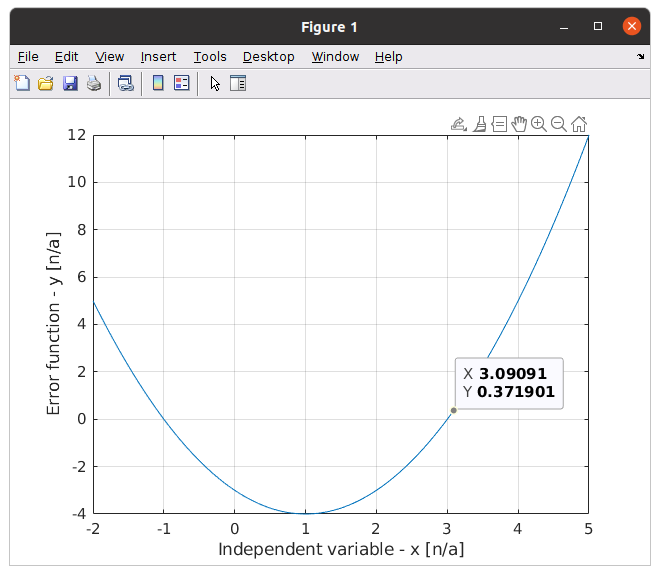
\includegraphics[width=0.7\textwidth]{images/error_w_data.png}}
    \caption{Visualization of the error function.}
    \label{f:error_data}
\end{figure}


    \subsection{Vectorizing Functions}

\index{vectorizing}
\index{function!vectorizing}

When you call the plotting script, you might get the following warning:

\begin{stdout}
Error using  ^ 
Incorrect dimensions for raising a matrix to a power. Check that the matrix
is square and the power is a
scalar. To operate on each element of the matrix individually, 
use POWER (.^) for elementwise power.
Error in error_func (line 2)
    res = x^2 - 2.*x -3;
Error in plot_error (line 3)
y = error_func(x); 
\end{stdout}

This means that MATLAB tried to call \lstinline{error_func} with a vector, and it failed.
The problem is that it uses the \lstinline{*} and \lstinline{^} operators which refer to matrix operations that follow the rules of linear algebra.  In this case this is not what we intended; instead we want to do \emph{element-wise} array multiplication and exponentiation (see ``\nameref{elementwise}'' on page~\pageref{elementwise}).

\index{element-wise operator}
\index{operator!element-wise}

If you rewrite \lstinline{error_func} like this:

\begin{code}
function res = error_func(x)
    res = x.^2 - 2.*x -3;
end
\end{code}
the warning message goes away.

\subsection{Anonymous Functions}

One way to avoid a separate M-file, \emph{error\_func.m}, for the function definition we provide to \lstinline{fzero} is to define an 
\href{https://www.mathworks.com/help/matlab/matlab_prog/anonymous-functions.html}{\emph{anonymous function}}.  
An anonymous function is a single statement function, not stored in a separate program file, associated with a function handle.  

\lstinputlisting[style=mcode_numbers]{w06_datatypes_fzero/lessons/fzero_afunc.m}

The second line defines the singe-expression anonymous function handle, \lstinline{error_afunc_handle}.  Then we pass the function handle to \lstinline{fzero}.  Note that the \lstinline{error_afunc_handle} variable stores a function handle - not a function.
\begin{code}
    >> whos
  Name                    Size            Bytes  Class              Attributes

  ans                     1x1                 8  double                       
  error_afunc_handle      1x1                32  function_handle    
\end{code}
This is the reason why there is no \lstinline{@} in the call to \lstinline{fzero}.

Anonymous function make the code more concise, avoiding having separate files for script and the function definition, but at the expense of readability.  Among other issues, the syntax for defining anonymous functions is less-than intuitive.  A better way of being concise while maintaining readability might be to use a local function.  Since R2024a, local functions can be anywhere in the script file, not just at the end, so an equivalent implementation would be...

\lstinputlisting[style=mcode_numbers]{w06_datatypes_fzero/lessons/fzero_demo_local.m}

It is still beneficial to be aware of anonymous functions.  You will likely run into online examples and documentation that uses anonymous functions, even if you don't write them yourself.

\section{How fzero Works}
\label{howfzero}

According to the MATLAB documentation, \lstinline{fzero} uses ``a combination of bisection, secant, and inverse quadratic interpolation methods.''  (See \url{https://greenteapress.com/matlab/fzero})

\index{fzero@\lstinline{fzero}}
\index{bisection}
\index{secant method}
\index{inverse quadratic interpolation}
\index{root}

To understand what that means, suppose we're trying to find a root of a function of one variable, $f(x)$, and assume we have evaluated the function at two places, $x_1$ and $x_2$, and found that the results have opposite signs.  Specifically, assume $f(x_1) > 0$ and $f(x_2) < 0$, as shown in Figure~\ref{fig:secant}.

\begin{figure}[h]
\centerline{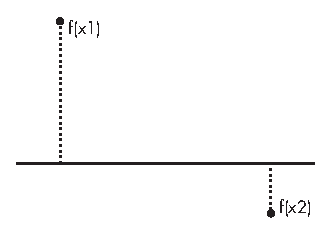
\includegraphics[scale=0.8]{images/figure15_03_new}}
\caption{Initial state of a root-finding search}
\label{fig:secant}
\end{figure}

As long as $f$ is continuous, there must be at least one root in this interval.
In this case we would say that $x_1$ and $x_2$ \emph{bracket} a zero.

\index{bracket}

If this were all you knew about $f$, where would you go looking for
a root?  If you said ``halfway between $x_1$ and $x_2$,''
congratulations!  You just invented a numerical method called
\emph{bisection}!

If you said, ``I would connect the dots with a straight line
and compute the zero of the line,''
congratulations!  You just invented the \emph{secant method}!

And if you said, ``I would evaluate $f$ at a third point, find the
parabola that passes through all three points, and compute the zeros
of the parabola,'' congratulations, you just invented
\emph{inverse quadratic interpolation}!

That's most of how \lstinline{fzero} works.  The details of how these methods are combined are interesting, but beyond the scope of this book.  You can read more at \url{https://greenteapress.com/matlab/brent}.




\section{Debugging}

When you start writing longer programs, you might spend more time debugging.  So we'll end this chapter with some debugging tips.

\subsection{More Name Collisions}

Functions and variables occupy the same workspace, which means
that whenever a name appears in an expression, MATLAB starts by looking
for a variable with that name; if there isn't one, it looks for
a function.

\index{name collision}
\index{collision!name}
\index{shadow}

As a result, if you have a variable with the same name as a function,
the variable \emph{shadows} the function; metaphorically, you can't see the function because the variable is in the way.

For example, if you assign
a value to \lstinline{sin} and then try to use the \lstinline{sin} function, you
might get an error:

\begin{code}
>> sin = 3;
>> sin(5)
Index exceeds the number of array elements (1).

'sin' appears to be both a function and a variable.
If this is unintentional, use 'clear sin' to remove
the variable 'sin' from the workspace.
\end{code}

Since the value we assigned to \lstinline{sin} is a number, and a number is considered a $1 \times 1$ matrix, MATLAB tries to access the fifth element of the matrix and finds that there isn't one.

In this case, MATLAB is able to detect the error, and the error message is pretty helpful.
But if the value of \lstinline{sin} were a vector, or if the argument were smaller, you would be in trouble.  For example,

\begin{code}
>> sin = 3;
>> sin(1)
ans = 3
\end{code}

Just to review, the sine of 1 is not 3!

You can avoid these problems by choosing function names carefully. Use long, descriptive names for functions, not single letters like \lstinline{f}. To be even clearer, use function names that end in \lstinline{func}. And before you define a function, check whether MATLAB already has a function with the same name.

\subsection{Debugging Your Head}

When you're working with a new function or a new language feature
for the first time, you should test it in isolation before you
put it into your program.

\index{debugging}

For example, suppose you know that \lstinline{x} is the sine of some
angle and you want to find the angle.  You find the MATLAB function
\lstinline{asin}, and you're pretty sure it computes the inverse sine
function.  Pretty sure is not good enough; you want to be very sure.

Since we know $\sin 0 = 0$, we could try

\begin{code}
>> asin(0)
ans = 0
\end{code}
which is correct.  Now, we also know that the sine of $90$\textdegree is
1, so if we try \lstinline{asin(1)}, we expect the answer to be 90, right?

\begin{code}
>> asin(1)
ans = 1.5708
\end{code}

Oops.  We forgot that the trig functions in MATLAB work in radians,
not degrees.  The answer we got is $\pi/2$, which is $90$\textdegree, in radians.

With this kind of testing, you're not really checking for
errors in your program; you're checking your understanding.  If you
make an error because you are confused about how MATLAB works, it
might take a long time to find, because when you look at the code,
it looks right.

\index{debugging!Seventh Theorem}

Which brings us to the Seventh Theorem of Debugging:

\begin{quote}
The worst bugs aren't in your code; they're in your head.
\end{quote}

\section{Chapter Review}

This chapter introduced \lstinline{fzero}, a function we can use to solve nonlinear equations.
To use \lstinline{fzero}, you have to write an error function and pass a function handle as an argument.  Using functions in this way can be tricky at first, but get comfortable with it, because we are going to use it a lot.

Here are some terms from this chapter you might want to remember.

If we can solve an equation by performing algebraic operations and deriving an explicit way to compute a value, the result is an \emph{analytic solution}.
Otherwise, we can use a \emph{numerical method}, which finds a \emph{numerical solution} to the equation, which is usually an approximation.

To solve nonlinear equations, we often rewrite them as functions and then find one or more \emph{zeros} of the function, that is, arguments that make the value of the function $0$.

A \emph{function handle} is a way of
referring to a function by name (and passing it as an argument)
without calling it.

A \emph{anonymous function} is a single-expression function definition, not defined in its own separate file, where the resulting function handle is assigned to a variable.

Finally, \emph{shadowing} is a kind of name collision in which a new definition
causes an existing definition to become invisible.  In MATLAB,
variable names can shadow built-in functions (with hilarious results).

In the next chapter, we'll write functions that take vectors as inputs and return vectors as outputs.


\section{Exercises}

Before you go on, you might want to work on the following exercises.

\begin{ex}

\begin{enumerate}

\index{Chebyshev polynomial}

\item Write a function called \lstinline{cheby6} that evaluates the
sixth Chebyshev polynomial.  It should take an input variable,
$x$, and return

\begin{equation*}
32 x^6 - 48 x^4 + 18 x^2 - 1
\end{equation*}

\item Use \lstinline{plot} to display a graph of this function in the
interval from $-1$ to $1$.  Estimate the location of any zeros in this
range.

\item Use \lstinline{fzero} to find as many different roots as you can.
Does \lstinline{fzero} always find the root that is closest to the initial
value?

\end{enumerate}

% cheby6.m
\end{ex}


\begin{ex}
\label{ex:duck}

When a duck is floating on water, how much of its body is submerged?\footnote{This exercise is adapted from C.~F.~Gerald and P.~O.~Wheatley, \emph{Applied Numerical Analysis}, 4th edition (Boston: Addison-Wesley, 1989).}

\index{duck}
\index{sphere}

To estimate a solution to this problem, we'll assume that the submerged part of a duck is well approximated by a section of a sphere.
If a sphere with radius $r$ is submerged in water to a depth $d$, the
volume of the sphere below the water line is

\[ V = \frac{\pi}{3} (3r d^2 - d^3) \quad
\mbox{as long as} \quad d < 2 r  \]

We'll also assume that the density of a duck is $\rho = 0.3$\,g/cm$^3$ (0.3 times the density of water) and that its mass is $\frac{4}{3} \pi r^3 \rho$\,g.

Finally, according to the law of buoyancy, an object floats at the level where the weight of the displaced water equals the total weight of the object.

\index{density}
\index{buoyancy}

Here are some suggestions for how to proceed:

\begin{enumerate}

\item Write an equation relating $\rho$, $d$, and $r$.

\item Rearrange the equation so the right-hand side is zero.
Our goal is to find values of $d$ that are roots of this equation.

\item Write a MATLAB function that evaluates this function.  Test it,
   then make it a quiet function.

\item Make a guess about the value of $d_0$ to use as an initial value.

\item Use \lstinline{fzero} to find a root near $d_0$.

\item Check to make sure the result makes sense.  In particular,
   check that $d < 2 r$, because otherwise the volume equation
   doesn't work!

\item Try different values of $\rho$ and $r$ and see if you get the
  effect you expect.  What happens as $\rho$ increases?  Goes to
  infinity?  Goes to zero?  What happens as $r$ increases?  Goes to
  infinity?  Goes to zero?

\end{enumerate}


% TODO: Find places in the book where error messages are getting syntax highlighting, and put them in a verbatim environment.


\end{ex}

\chapter{Functions of Vectors}


Now that we have functions and vectors, we'll put them together to write functions that take vectors as input variables and return vectors as output variables.  You'll also see two patterns for computing with vectors: existential and universal quantification.


\section{Functions and Vectors}

In this section we'll look at common patterns involving functions and vectors, and you will learn how to write a single function that can work with \mbox{vectors} as well as scalars.

\subsection{Vectors as Input Variables}

Since many of the built-in functions take vectors as arguments,
it should come as no surprise that you can write functions that
take vectors as input.  Here's a simple (but not very useful) example:

\index{vector}
\index{input variable}

\begin{code}
function res = display_vector(X)
    for i=1:length(X)
        display(X(i))
    end
end
\end{code}

There's nothing special about this function.  The only
difference from the scalar functions we've seen is that this one uses
a capital letter to remind us that \lstinline{X} is a vector.

Using \lstinline{display_vector} doesn't actually return a value; it just displays the elements of the vector it gets as an input variable:

\begin{code}
>> display_vector(1:3)
    1
    2
    3
\end{code}

Here's a more interesting example that encapsulates the code
from Listing~\ref{lst:vec_reduce} on page~\pageref{lst:vec_reduce} to add up the elements of a vector:

\index{encapsulation}

\begin{code}
function res = mysum(X)
    total = 0;
    for i=1:length(X)
        total = total + X(i);
    end
    res = total;
end
\end{code}

I called this function \lstinline{mysum} to avoid a collision with the built-in
function \lstinline{sum}, which does pretty much the same thing.

\index{sum@\lstinline{sum}}

Here's how you call it from the Command Window:

\begin{code}
>> total = mysum(1:3)
total = 6
\end{code}

Because this function has an output variable, I made a
point of assigning it to a variable.

\index{output variable}


\subsection{Vectors as Output Variables}

There's also nothing wrong with assigning a vector to an output
variable. Here's an example that encapsulates the code from
Listing~\ref{lst:vec_apply} on page~\pageref{lst:vec_apply}:

\begin{code}
function res = mysquare(X)
    for i=1:length(X)
        Y(i) = X(i)^2;
    end
    res = Y;
end
\end{code}

This function squares each element of \lstinline{X} and stores it as an element of \lstinline{Y}.  Then it assigns \lstinline{Y} to the output variable, \lstinline{res}.  Here's how we use this function:
\index{apply}

\begin{code}
>> V = mysquare(1:3)
V = 1     4     9
\end{code}

The input variable is a vector with the elements \lstinline{1,2,3}.  The output variable is a vector with the elements \lstinline{1,4,9}.




\subsection{Vectorizing Functions}

Functions that work on vectors will almost always work on scalars
as well, because MATLAB considers a scalar to be a vector with
length 1.

\index{vectorizing}
\index{function!vectorizing}

\begin{code}
>> mysum(17)
ans = 17

>> mysquare(9)
ans = 81
\end{code}

Unfortunately, the converse isn't always true.  If you write
a function with scalar inputs in mind, it might not work on vectors.

But it might!  If the operators and functions
you use in the body of your function work on vectors, then your
function will probably work on vectors.
For example, here's the very first function we wrote:

\begin{code}
function res = myfunc(x)
    s = sin(x);
    c = cos(x);
    res = abs(s) + abs(c);
end
\end{code}

And lo!  It turns out to work on vectors because the MATLAB basic functions we used in \lstinline{myfunc}, \lstinline{sin, cos, abs} all work with vectors:

\begin{code}
>> Y = myfunc(1:3)
Y = 1.3818    1.3254    1.1311
\end{code}

Some other functions we wrote don't work on vectors,
but they can be patched up with just a little effort.  For example,
here's \lstinline{hypotenuse} from Section~\ref{hypotenuse_exercise}:

\begin{code}
function res = hypotenuse(a, b)
    res = sqrt(a^2 + b^2);
end
\end{code}

This doesn't work on vectors because the \lstinline{^} operator
defaults to matrix operations, using linear algebra, which only works on
square matrices.

\index{matrix exponentiation}

\begin{code}
>> hypotenuse(1:3, 1:3)
Error using  ^  (line 51)
Incorrect dimensions for raising a matrix to a power.
Check that the matrix is square and the power is a scalar.
To perform element-wise matrix powers, use '.^'.
\end{code}

But convert this to use the element-wise array operation by replacing \lstinline{^} with the element-wise operator
(\lstinline{.^}), it works!

\index{element-wise operator}

\begin{code}
>> A = [3,5,8];
>> B = [4,12,15];
>> C = hypotenuse(A, B)

C = 5    13    17
\end{code}

The function matches up corresponding elements from the two
input vectors, so the elements of \lstinline{C} are the hypotenuses of
the pairs $(3,4)$, $(5,12)$, and $(8,15)$, respectively.

In general, if you write a function using only element-wise
operators and functions that work on vectors, the new
function will also work on vectors.


\subsection{Sums and Differences}

Another common vector operation is \emph{cumulative sum}, which takes a vector as an input and computes a new vector that contains all the partial sums of the original.  In math notation, if $V$ is the original vector, the elements of the cumulative sum, $C$, are

\index{cumulative sum}
\index{sum!cumulative}

\begin{equation*}
C_i = \sum_{j=1}^i V_j
\end{equation*}

In other words, the $i$th element of $C$ is the sum of the first
$i$ elements from $V$.  MATLAB provides a function named \lstinline{cumsum} that computes cumulative sums:

\index{cumsum@\lstinline{cumsum}}

\begin{code}
>> X = 1:5

X = 1     2     3     4     5

>> C = cumsum(X)

C = 1     3     6    10    15
\end{code}

The inverse operation of \lstinline{cumsum} is \lstinline{diff}, which computes
the difference between successive elements of the input vector.

\index{diff@\lstinline{diff}}

\begin{code}
>> D = diff(C)

D = 2     3     4     5
\end{code}

Notice that the output vector is shorter by one than the input
vector.  As a result, MATLAB's version of \lstinline{diff} is not
exactly the inverse of \lstinline{cumsum}.  If it were, we would
expect \lstinline{cumsum(diff(X))} to be \lstinline{X}:

\begin{code}
>> cumsum(diff(X))

ans = 1     2     3     4
\end{code}

But it isn't.

\begin{ex}
Write a function named \lstinline{mydiff} that computes the
inverse of \lstinline{cumsum} so that \lstinline{cumsum(mydiff(X))} and
\lstinline{mydiff(cumsum(X))} both return \lstinline{X}.

% mydiff.m
\end{ex}


\subsection{Products and Ratios}

The multiplicative version of \lstinline{cumsum} is \lstinline{cumprod},
which computes the \emph{cumulative product}.  In math notation,
that's

\index{cumulative product}
\index{product!cumulative}
\index{cumprod@\lstinline{cumprod}}

\begin{equation*}
P_i = \prod_{j=1}^i V_j
\end{equation*}

In MATLAB, that looks like

\begin{code}
>> V = 1:5

V = 1     2     3     4     5

>> P = cumprod(V)

P = 1     2     6    24   120
\end{code}

MATLAB doesn't provide the multiplicative version
of \lstinline{diff}, which would be called \lstinline{ratio}, and which would
compute the ratio of successive elements of the input vector.

\begin{ex}
Write a function named \lstinline{myratio} that computes the
inverse of \lstinline{cumprod}, so that \lstinline{cumprod(myratio(X))} and
\lstinline{myratio(cumprod(X))} both
return \lstinline{X}.

You can use a loop, or if you want to be clever, you can take
advantage of the fact that $e^{\ln a + \ln b} = a b$.

%If you apply \lstinline{myratio} to a vector that contains Fibonacci numbers, you can confirm that the ratio of successive elements converges on the golden ratio, $(1+\sqrt{5})/2$ (see Section~\ref{fibratio}).

\end{ex}


\section{Computing with Vectors}

In this section, we'll look at two common patterns for working with vectors and connect them to the corresponding ideas from mathematics, existential and universal quantification.  And you'll learn about logical vectors, which contain the Boolean values 0 and 1.

\subsection{Existential Quantification}

\index{existential quantification}
\index{quantification!existential}

It's often useful to check the elements of a vector to see if there
are any that satisfy a condition.  For example, you might want to
know if there are any positive elements.  In mathematical terms, checking whether something exists is called \emph{existential quantification}, and it's denoted with
the symbol $\exists$, which is pronounced ``there exists.''  For example,
% this expression
%
\[ \exists x \mbox{~in~} S: x>0  \]
%
means, ``there exists some element $x$ in the set $S$ such that
$x>0$.''  In MATLAB, it's natural to express this idea with a logical
function, like \lstinline{exists}, that returns \lstinline{1} if there is such an
element and \lstinline{0} if there is not.

\begin{code}
function res = exists(X)
    for i=1:length(X)
        if X(i) > 0
            res = 1;
            return
        end
    end
    res = 0;
end
\end{code}

We haven't seen the \lstinline{return} statement before ; it's similar
to \lstinline{break} except that it breaks out of the whole function, not
just the loop.  That behavior is what we want here because as soon
as we find a positive element, we know the answer (it exists!) and
we can end the function immediately without looking at the rest
of the elements.

\index{return statement@\lstinline{return} statement}
\index{statement!return@\lstinline{return}}

If we get to the end of the loop, that means we didn't find what
we were looking for, so the result is \lstinline{0}.

\subsection{Universal Quantification}

\index{universal quantification}
\index{quantification!universal}

Another common operation on vectors is to check whether \emph{all} the elements satisfy a condition, which is called \emph{universal quantification}, denoted with
the symbol $\forall$ and pronounced ``for all.''  So the expression % this expression
%
\[ \forall x \mbox{~in~} S: x>0 \]
%
means ``for all elements $x$ in the set $S$, $x>0$.''

One way to evaluate this expression in MATLAB is to reduce the problem to
existential quantification, that is, to rewrite

\begin{equation*}
\forall x \mbox{~in~} S: x>0
\end{equation*}
to the following:
\begin{equation*}
{\sim} \exists x \mbox{~in~} S: x \le 0
\end{equation*}
where ${\sim} \exists$ means ``does not exist.''
In other words, checking that all the  elements are positive is
the same as checking that there are no elements
that are nonpositive.

\begin{ex}
Write a function named \lstinline{forall} that
takes a vector and returns \lstinline{1} if all the elements are positive
and \lstinline{0} if there are any non-positive elements.

\end{ex}

\subsection{Logical Vectors}

When you apply a logical operator to a vector, the result is a
\emph{logical vector}: a vector whose elements are the logical
values 1 and 0. Let's look at an  example:

\index{logical vector}
\index{vector!logical}

\begin{code}
>> V = -3:3

V = -3    -2    -1     0     1     2     3

>> L = V>0

L =  0     0     0     0     1     1     1
\end{code}

In this example, \lstinline{L} is a logical vector whose elements
correspond to the elements of \lstinline{V}.  For each positive element of
\lstinline{V}, the corresponding element of \lstinline{L} is \lstinline{1}.

Logical vectors can be used like flags to store the state of
a condition.  And they are often used with the \lstinline{find} function,
which takes a logical vector and returns a vector that contains
the indices of the elements that are ``true.''

\index{flag}
\index{find@\lstinline{find}}

Applying \lstinline{find} to \lstinline{L} from the example above yields

\begin{code}
>> find(L)

ans = 5     6     7
\end{code}
which indicates that elements 5, 6, and 7 have the value 1.

If there are no ``true'' elements, the result is an empty vector.

\begin{code}
>> find(V>10)

ans = Empty matrix: 1x0
\end{code}

This example computes the logical vector and passes it as an
argument to \lstinline{find} without assigning it to an intermediate
variable.  You can read this version abstractly as ``find
the indices of elements of \lstinline{V} that are greater than~10.''

We can also use \lstinline{find} to write \lstinline{exists} more concisely:

\begin{code}
function res = exists(X)
    L = find(X>0)
    res = length(L) > 0
end
\end{code}

\begin{ex}
Write a version of \lstinline{forall} using \lstinline{find}.
\end{ex}


\section{Debugging in Four Acts}

\index{debugging}
\index{reading}
\index{running}
\index{ruminating}
\index{retreating}

When you're debugging a program, and especially if you're working on a hard bug, there are four things to try:

\begin{description}

\item[Reading] Examine your code, read it back to yourself, and
check that it means what you meant to say.

\item[Running] Experiment by making changes and running different
versions.  Often, if you display the right thing at the right place
in the program, the problem becomes obvious, but you might have to invest time building scaffolding.

\item[Ruminating] Take some time to think!  What kind of error
is it: syntax, runtime, or logical?  What information can you get from
the error messages or from the output of the program?  What kind of
error could cause the problem you're seeing?  What did you change
last, before the problem appeared?

\item[Retreating] At some point, the best thing to do is back
off, undoing recent changes, until you get back to a program that
works and that you understand.  Then you can start rebuilding.

\end{description}

Beginning programmers sometimes get stuck on one of these activities
and forget the others.  Each activity comes with its own failure
mode.
For example, reading your code might help if the problem is a
typographical error, but not if the problem is a conceptual
misunderstanding.  If you don't understand what your program does, you
can read it 100 times and never see the error, because the error is in
your head.

Running experiments can help, especially if you run small, simple
tests.  But if you run experiments without thinking or reading your
code, you might fall into a pattern I call ``random walk programming,''
which is the process of making random changes until the program
does the right thing.  Needless to say, random walk programming
can take a long time.

\index{random walk programming}

The way out is to take more time to think.  Debugging is like an
experimental science.  You should have at least one hypothesis about
what the problem is.  If there are two or more possibilities, try to
think of a test that would eliminate one of them.

\index{hypothesis}

Taking a break sometimes helps with the thinking.  So does talking.
If you explain the problem to someone else (or even yourself), you
will sometimes find the answer before you finish asking the question.

But even the best debugging techniques will fail if there are too many
errors or if the code you are trying to fix is too big and
complicated.  Sometimes the best option is to retreat, simplifying the
program until you get to something that works, and then rebuild.

Beginning programmers are often reluctant to retreat, because
they can't stand to delete a line of code (even if it's wrong).
If it makes you feel better, copy your program into another file
before you start stripping it down.  Then you can paste the pieces
back in, a little bit at a time.

\index{debugging!Eighth Theorem}

To summarize, here's the Eighth Theorem of Debugging:

\begin{quote}
Finding a hard bug requires reading, running, ruminating,
and sometimes retreating.  If you get stuck on one of these
activities, try the others.
\end{quote}

\section{Chapter Review}

This chapter presents patterns for working with vectors, including existential and universal quantification.
We learned how to write functions that take vectors as input variables and return vectors as output variables.
And we learned about \emph{logical vectors}, which contain the values 1 and 0 to represent true and false.

Some functions in this chapter are not idiomatic MATLAB; many of them can be done more simply using built-in MATLAB operators and functions, rather than writing them yourself.  But these examples demonstrate concepts you will need to know when you work on more complicated problems.

In the next chapter, we will apply the tools we have learned so far to the central goal of this book, modeling physical systems.



%\section{Exercises}

%\begin{ex}
%\end{ex}

%TODO: any exercises for this chapter?

\chapter{Ordinary Differential Equations}


In Exercise~\ref{ex:duck}, we found the equilibrium point where a duck would float on water.  This kind of problem is called \emph{static} because it does not move.  This chapter introduces \emph{dynamic} problems, which involve things that change over time.

Also, you'll learn about a mathematical tool for describing physical systems, \emph{differential equations}, and two computational tools for solving them, Euler's method and \lstinline{ode45}.

But first I have a quick suggestion about organizing code in files.

\section{Functions and Files}
\label{funfiles}

So far we've only put one function in each file.  It's also possible
to put more than one function in a file, but only the first one, the
\emph{main function}, can be called from the Command
Window.  The other \emph{local functions} can be called from anywhere inside the file, but not from the Command Window or any other file.

\index{function!main}
\index{main function}
\index{local function}
\index{function!local}

Keeping multiple functions in one file is convenient, but it makes  debugging
difficult because you can't call local functions from the Command
Window.

To help with this problem, I often use the top-level function
to develop and test my local functions.  For example, to write
a program for Exercise~\ref{ex:duck}, I would create a file named
\emph{duck.m} and start with a main function named \lstinline{duck}
that takes no input variables and returns no output value.

Then I would write a function named \lstinline{error_func} to
evaluate the error function for \lstinline{fzero}.  To test
\lstinline{error_func}, I would call it from \lstinline{duck} and then
call \lstinline{duck} from the Command Window.

\index{incremental development}

Here's what my first draft might look like:

\begin{code}
function res = duck()
    error = error_func(10)
end

function res = error_func(d)
    rho = 0.3;      % density in g / cm^3
    r = 10;         % radius in cm
    res = d;
end
\end{code}

This program is not complete, but it is enough code to test.
Once this program is working, I would finish writing \lstinline{error_func}.
And once I'd finished and tested \lstinline{error_func}, I would modify
\lstinline{duck} to use \lstinline{fzero}.

This problem might only require two functions, but if there
were more, I could write and test them one at a time and then
combine them into a working program.

Now, let's get back to differential equations.


\section{Differential Equations}
\label{diffeq}

A \emph{differential equation (DE)} is an equation that describes the
derivatives of an unknown function.  ``Solving a DE'' means finding a
function whose derivatives satisfy the equation.

\index{differential equation}
\index{equation!differential}

For example, suppose we would like to predict the population of yeast growing in a nutrient solution.  Assume that we know the initial population is 5 billion yeast cells.
When yeast grow in particularly yeast-friendly
conditions, the rate of growth at any point in time is proportional to the current population.  If we define $y(t)$ to be the population at a time $t$, we can write the following equation for the rate of growth:
%
\begin{equation*}
\frac{dy}{dt}(t) = a y(t)
\end{equation*}
%
where $\frac{dy}{dt}(t)$ is the derivative of $y(t)$ and
$a$ is a constant that characterizes how quickly the population
grows.
This equation is \emph{differential} because it relates a function to one of its derivatives.

\index{ordinary differential equation (ODE)}
\index{partial differential equation (PDE)}

It is an \emph{ordinary differential equation (ODE)} because all the
derivatives involved are taken with respect to the
same variable.
If it related derivatives with respect to
different variables (partial derivatives), it would be a \emph{partial
differential equation (PDE)}.

\index{differential equation!first-order}

This equation is \emph{first order} because it involves only first
derivatives.  If it involved second derivatives, it would be second order,
and so on.

\index{linear differential equation}

Lastly, it's \emph{linear} because each term involves $t$, $y$, or
$dy/dt$ raised to the first power; if any of the terms involved
products or powers of $t$, $y$, or $dy/dt$ it would be
\emph{nonlinear}.

Now suppose we want to predict the yeast population in the future.  We can do that using Euler's method.

\section{Euler's Method}

Here's a test to see if you're as smart as Leonhard Euler.  Let's say you arrive at time (~$t$) and measure the current population ($y$) and
the rate of change ($r$).  What do you think the population will
be after some period of time $\Delta t$  has elapsed?

If you said $y + r \Delta t$, congratulations!  You just invented
Euler's method.

\index{Euler's method}

This estimate is based on the assumption that $r$ is constant, but in general it's not, so we only expect the estimate to be good if $r$ changes slowly and $\Delta t$ is small.

What if we want to make a prediction when $\Delta t$ is large?
One option is to break $\Delta t$ into smaller pieces, called
\emph{time steps}. Then we can use the following equations to get from one time step to the next:
\begin{equation}
    \label{e:euler}
    \begin{array}{r@{}l}
        tt_{i+1} &{}= tt_i + dt   \\
        yy_{i+1} &{}= yy_i + \frac{df}{dt}(t) \, dt        
    \end{array}
\end{equation}

Here, $tt_i$ is a vector of times when we estimate the value of $y$, and $yy_i$ is the vector of estimates.
For each index $i$, $yy_i$ is an estimate of $y(tt_i)$.

\index{time step}

If the rate doesn't change too fast and the time step isn't
too big, Euler's method is accurate enough for most purposes.

%One
%way to check is to run it once with time step $dt$ and then run it
%again with time step $dt/2$.  If the results are the same, they are
%probably accurate, as . . .; otherwise, we can cut the time step again.


\section{Implementing Euler's Method}

As an example we'll use Euler's method to solve Equation~\ref{e:euler},
\[ \frac{dy}{dt}(t) = a y(t) \]
with the initial condition $y(0) = \SI{5}{cells}$  and
the growth parameter $a = \SI{0.2}{cells/hr}$.

\index{main function}

As a first step, create a file named \emph{euler.m} with a main function and a local function:

\begin{code}
function res = euler()
    tt(1) = 0;
    yy(1) = 5;
    r = rate_func(tt(1), yy(1))
end

function res = rate_func(t, y)
   a = 0.2;
   dydt = a * y;
   res = dydt;
end
\end{code}

In \lstinline{euler} we initialize the initial conditions and then call \lstinline{rate_func}, so called because it computes the rate of growth in the population.

\index{initial condition}

After testing these functions, we can add code to \lstinline{euler} to compute these difference equations:
\begin{eqnarray*}
tt_{i+1} &=&tt_i + \Delta t             \\
yy_{i+1} &=& yy_i + r \Delta t
\end{eqnarray*}
%
where $r$ is the rate of growth computed by \lstinline{rate_func}.
Listing~\ref{lst:euler_method} has the code we need:

\lstinputlisting[style=mcode, caption={A function implementing Euler's method}, label={lst:euler_method}]{w07_funcvectors_odes/lessons/euler.m}

Before the loop, we create two vectors, \lstinline{tt} and \lstinline{yy}, and set the first element of each with the initial conditions;  \lstinline{dt}, which is the size of the time steps, is \SI{0.1}{hours}.

Inside the loop, we compute the growth rate based on the current time, \lstinline{tt(i)}, and population, \lstinline{tt(i)}.  You might notice that the rate depends only on population, but we pass time as an input variable anyway, for reasons you'll see soon.

After computing the growth rate, we add an element both \lstinline{tt} and \lstinline{yy}, increasing their length by one.  Then, when the loop exits, we plot \lstinline{yy} as a function of \lstinline{tt}, adding labels and units as good engineering practice.

If you run the code, you should get a plot of population over time, as shown in Figure~\ref{fig:euler}.

\begin{figure}[ht!]
\centerline{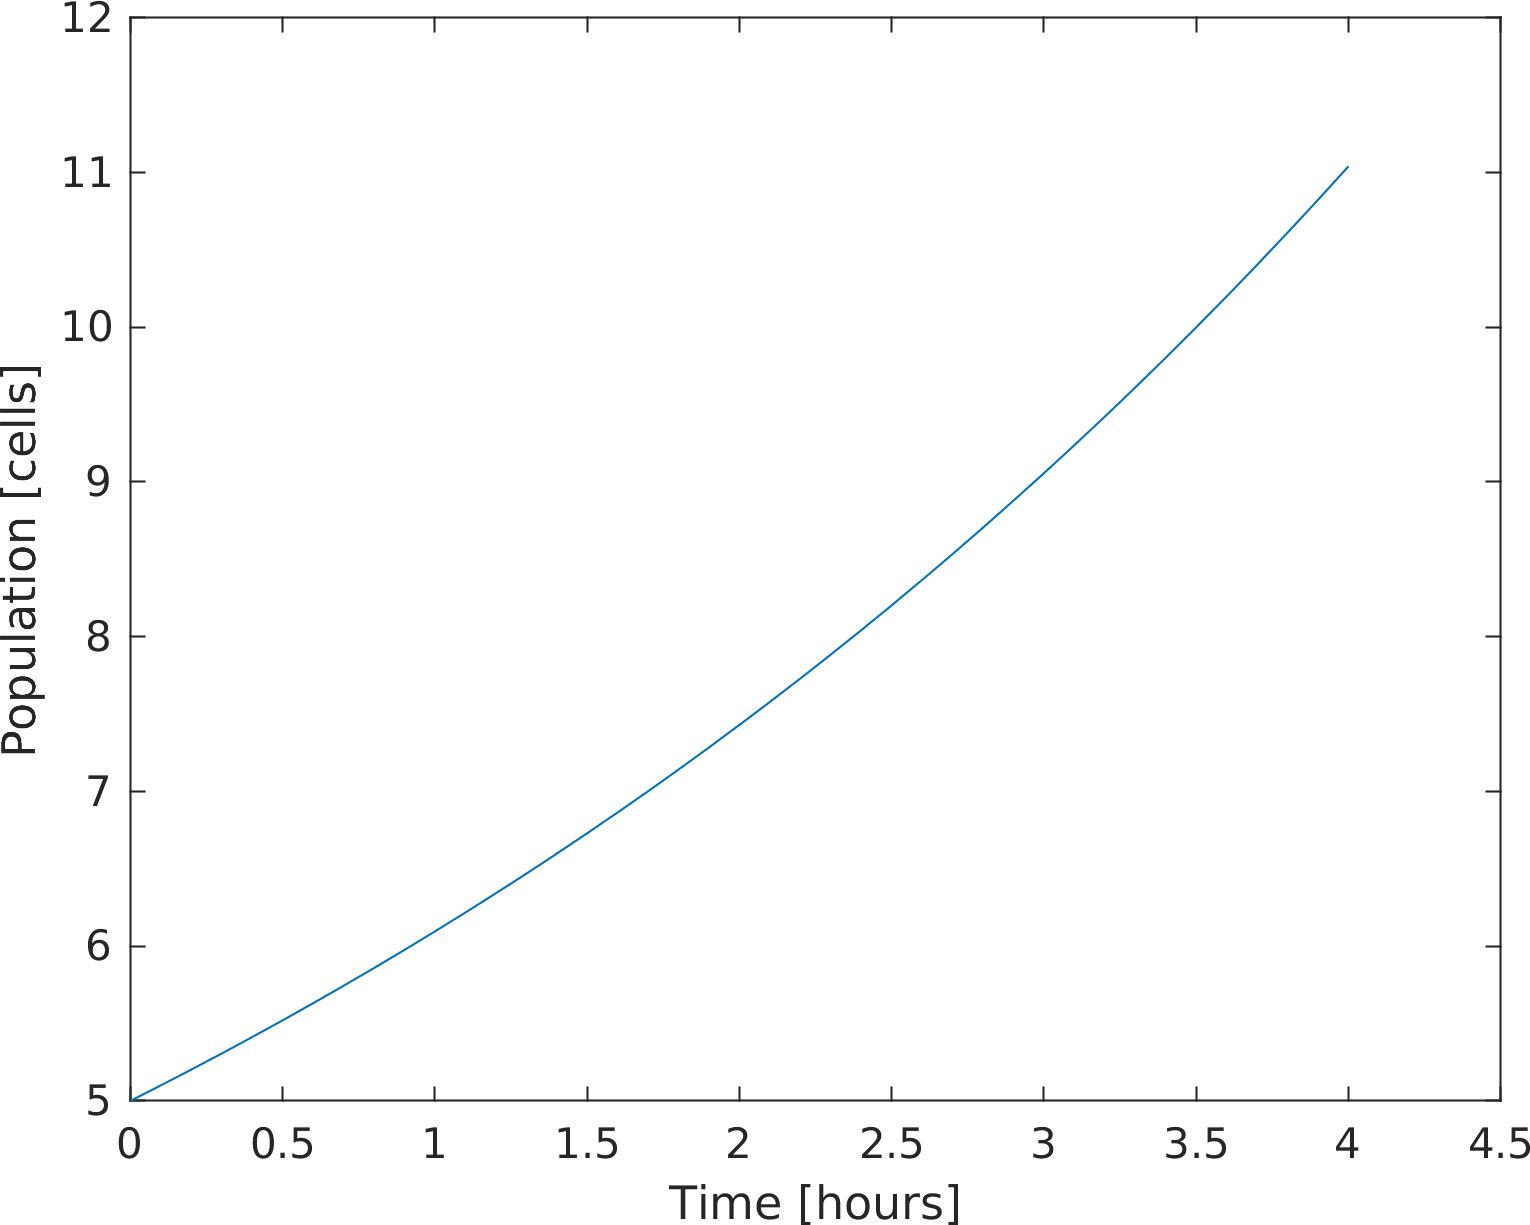
\includegraphics[width=0.7\textwidth]{images/euler.png}}
\caption{Solution to a simple differential equation by Euler's method}
\label{fig:euler}
\end{figure}

As you can see, the population doubles in a little less than 4 hours.  (You may recall for differential equations that for a linear, first-order system, the doubling time is $t_d = \ln(2)/r  = \ln(2)/0.2 = \SI{3.5}{s}$.)

\clearpage

\section{Solving ODEs with ode45}
\label{ode45}

A limitation of Euler's method is that it assumes that the derivative is constant between time steps, and that's not generally true.  Fortunately, there are better methods that estimate the derivative between time steps, and  they can be much more accurate.

\index{time step}
\index{ode45@\lstinline{ode45}}

MATLAB provides a function called \lstinline{ode45} that implements one of these methods.  In this section I'll explain how to use it; you can read more about how it works in Section~\ref{s:howode45} on page~\pageref{s:howode45}.

\index{rate function}
\index{function!rate}

In order to use \lstinline{ode45}, you have to write a function that evaluates $dy/dt$ as a function of $t$ and $y$.  Fortunately, we already have one, called \lstinline{rate_func}:

\begin{code}
function res = rate_func(t, y)
   a = 0.2;
   dydt = a * y;
   res = dydt;
end
\end{code}

We can call \lstinline{ode45} from the Command Window like this:

\begin{code}
[T, Y] = ode45(@rate_func, [0, 4], 5);
plot(T, Y)
\end{code}

The first argument is a function handle, as we saw in Chapter~\ref{fzero}.  The second argument is the time interval where we want to evaluate the solution; in this case the interval is from $t=0$ to $t=4$ hours.  The third argument is the initial population, 5 cells.  The result is two vectors, a vector of time values for the solution and a vector of the same length with the solution.

\index{function handle}
\index{handle!function}
\index{output variable}
\index{variable!output}

The full example, as a live script, is as follows:
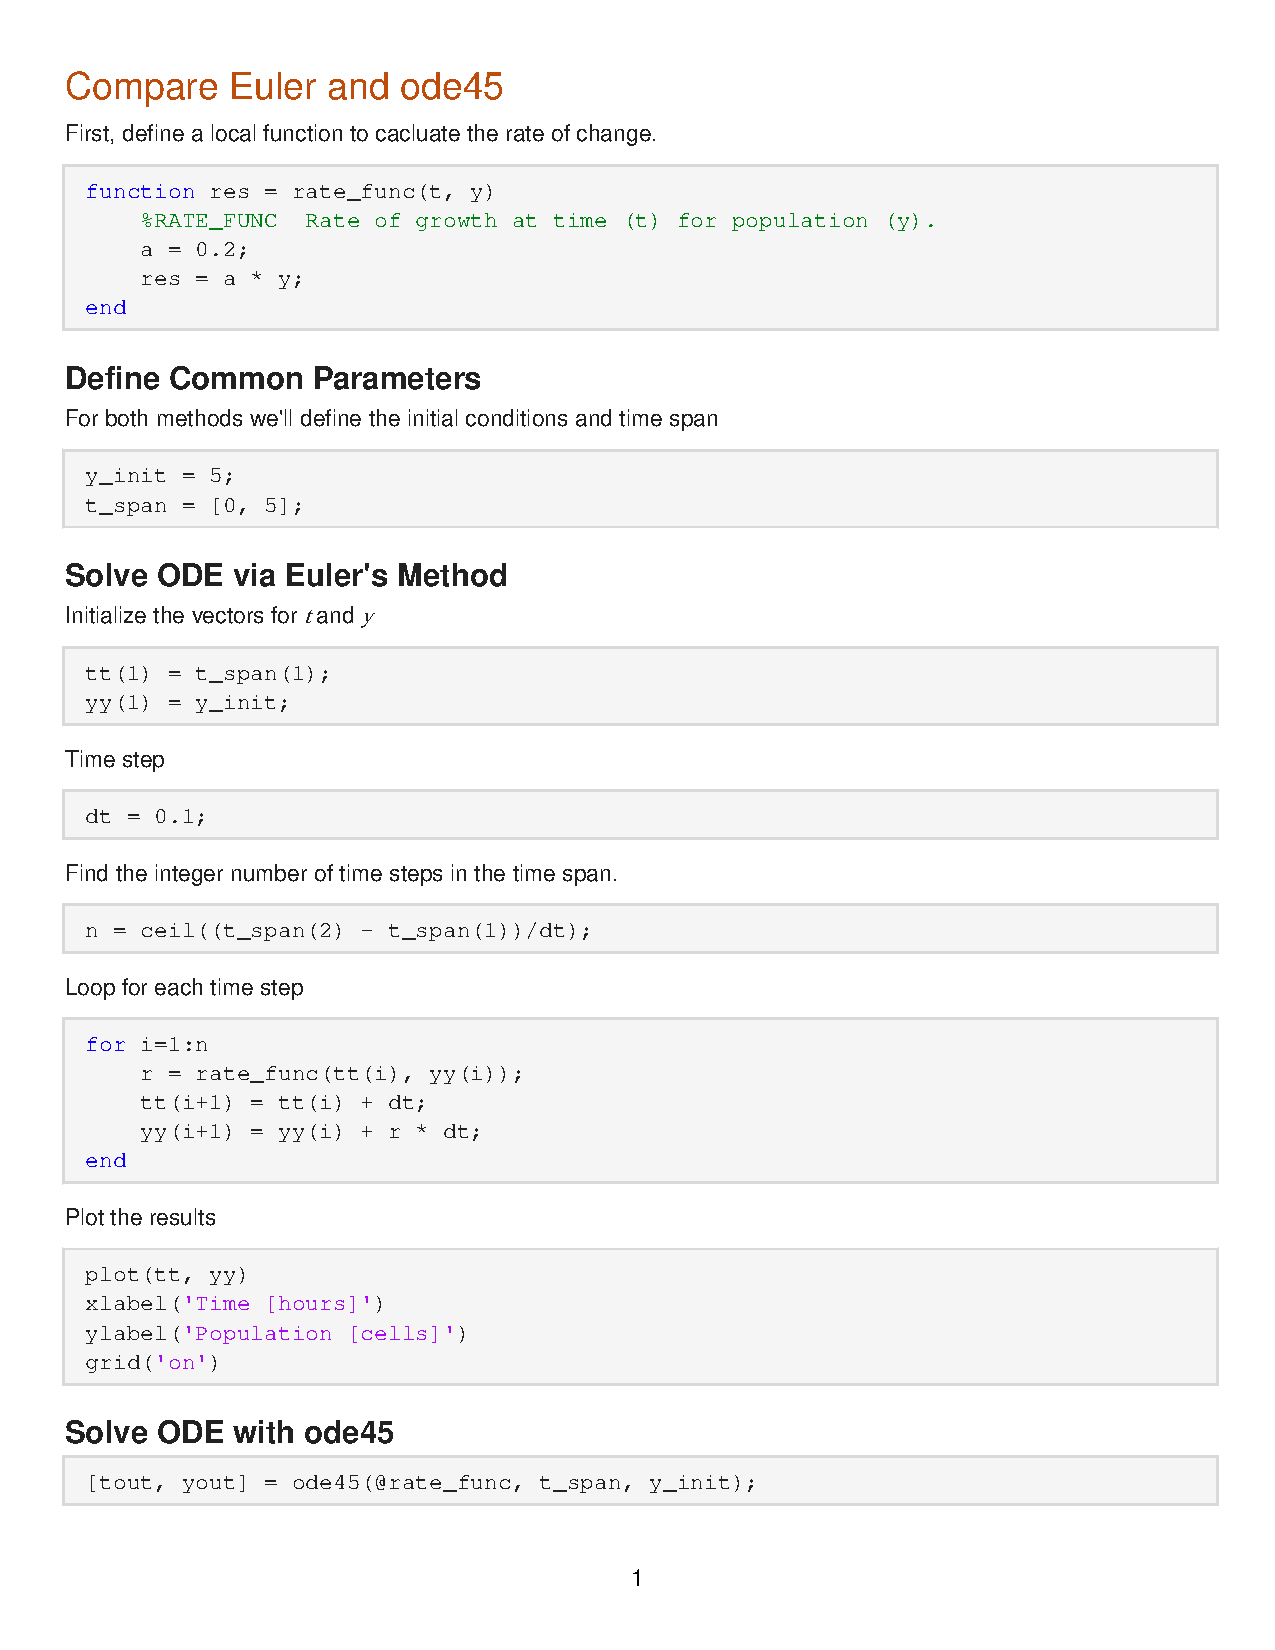
\includepdf[pages=-,frame,pagecommand={},width=\textwidth]{w07_funcvectors_odes/lessons/euler_compare.pdf}

The solid line is the estimate we computed with Euler's method; the dashed line is the solution from \lstinline{ode45}.

For the first 2--3 hours, the two solutions are visually indistinguishable.  During the last hour, they diverge slightly; at 4 hours, the difference is less than 1 percent.

For many purposes, the difference between Euler's method and \lstinline{ode45} is the least of our worries.  In this example, we probably don't know the initial population with perfect accuracy or the growth constant, \lstinline{a}.  Also, the assumption that the growth rate only depends on population is probably not true.  Any of these modeling errors could be bigger than 1 percent.

However, for some problems, Euler's method can be off by a lot more than 1 percent.
In those cases \lstinline{ode45} is almost always more accurate, for two reasons: first, it computes the rate function several times per time step; second, if the time step is too big, \lstinline{ode45} can detect the problem and shrink the time step.  For more details, see ``\nameref{s:howode45}'' on page~\pageref{s:howode45}.


\section{Time Dependence}

Looking at \lstinline{rate_func} in the previous section, you might notice that it takes \lstinline{t} as an input variable but doesn't use it.  That's because the growth rate does not depend on time---bacteria don't know what time it is.

\index{time dependence}

But rats do.  Or, at least, they know what season it is.
Suppose that the growth rate for rats depends on the current population \emph{and} the availability of food, which varies over the course of the year.
The differential equation might be something like
%
\begin{equation*}
\frac{dy}{dt}(t) = a y(t) \left(1 - \cos (\omega t) \right)
\end{equation*}
%
where $t$ is time in days and $y(t)$ is the population at time $t$.
Because the growth rate depends on time, this differential equation is \emph{time dependent}.

The variables $a$ and $\omega$ are \emph{parameters}, which are values that
quantify a physical aspect of the scenario.  Parameters are often constants, but in some models they vary in time.

\index{parameter}

In this example, $a$ characterizes the reproductive rate per day, and
$\omega$ is the frequency of a periodic function that describes
the effect of varying food supply on reproduction.

We'll use the values $a = \SI{0.002}{day^{-1}}$
and $\omega = 2 \pi / 365 \, \SI{}{rad/day}$ (one cycle per year).
The growth rate is lowest at $t=0$, on January~1, and highest at $t=365/2$, on June~30.

Now we can write a function that evaluates the growth rate:

\begin{code}
function res = rate_func(t, rats)
    %RATE_FUNC returns the growth rate at time (t) for population (rats)
    a = 0.002;
    omega = 2*pi / 365;
    res = a * rats * (1 - cos(omega * t));
end
\end{code}

To test this function, I put it in a file called \emph{rats.m} with a main function called
\lstinline{rats}:

\begin{code}
function res = rats_growth()
    t = 365/2;
    rats = 1000;
    res = rate_func(t, rats);
end
\end{code}

The main function assumes, for purposes of testing, that
there are 1000 rats at $t=365/2$ (June~30) and computes the growth rate under those conditions.

We can run the main function like this:

\begin{code}
>> r = rat_growth()

r = 4
\end{code}

Under these conditions, the growth rate is 4 new rats per day.

Now that we've tested \lstinline{rate_func}, we can use \lstinline{ode45} to solve the differential equation.
Here's how to call it from the main function in \emph{rats.m}:

\begin{code}
[tt, yy]] = ode45(@rate_func, [0, 365], 1000)
plot(tt, yy)
\end{code}

The first argument is a function handle, again.  The second argument is the interval we are interested in, a duration of one year, expressed in units of days.
The third argument is the initial population, $y(0) = 1000$.

\index{interval}

We can put this all together in the following program:
\lstinputlisting[style=mcode]{w07_funcvectors_odes/lessons/rat_growth.m}

Figure~\ref{fig:rats} shows the results.

\begin{figure}[ht]
\centerline{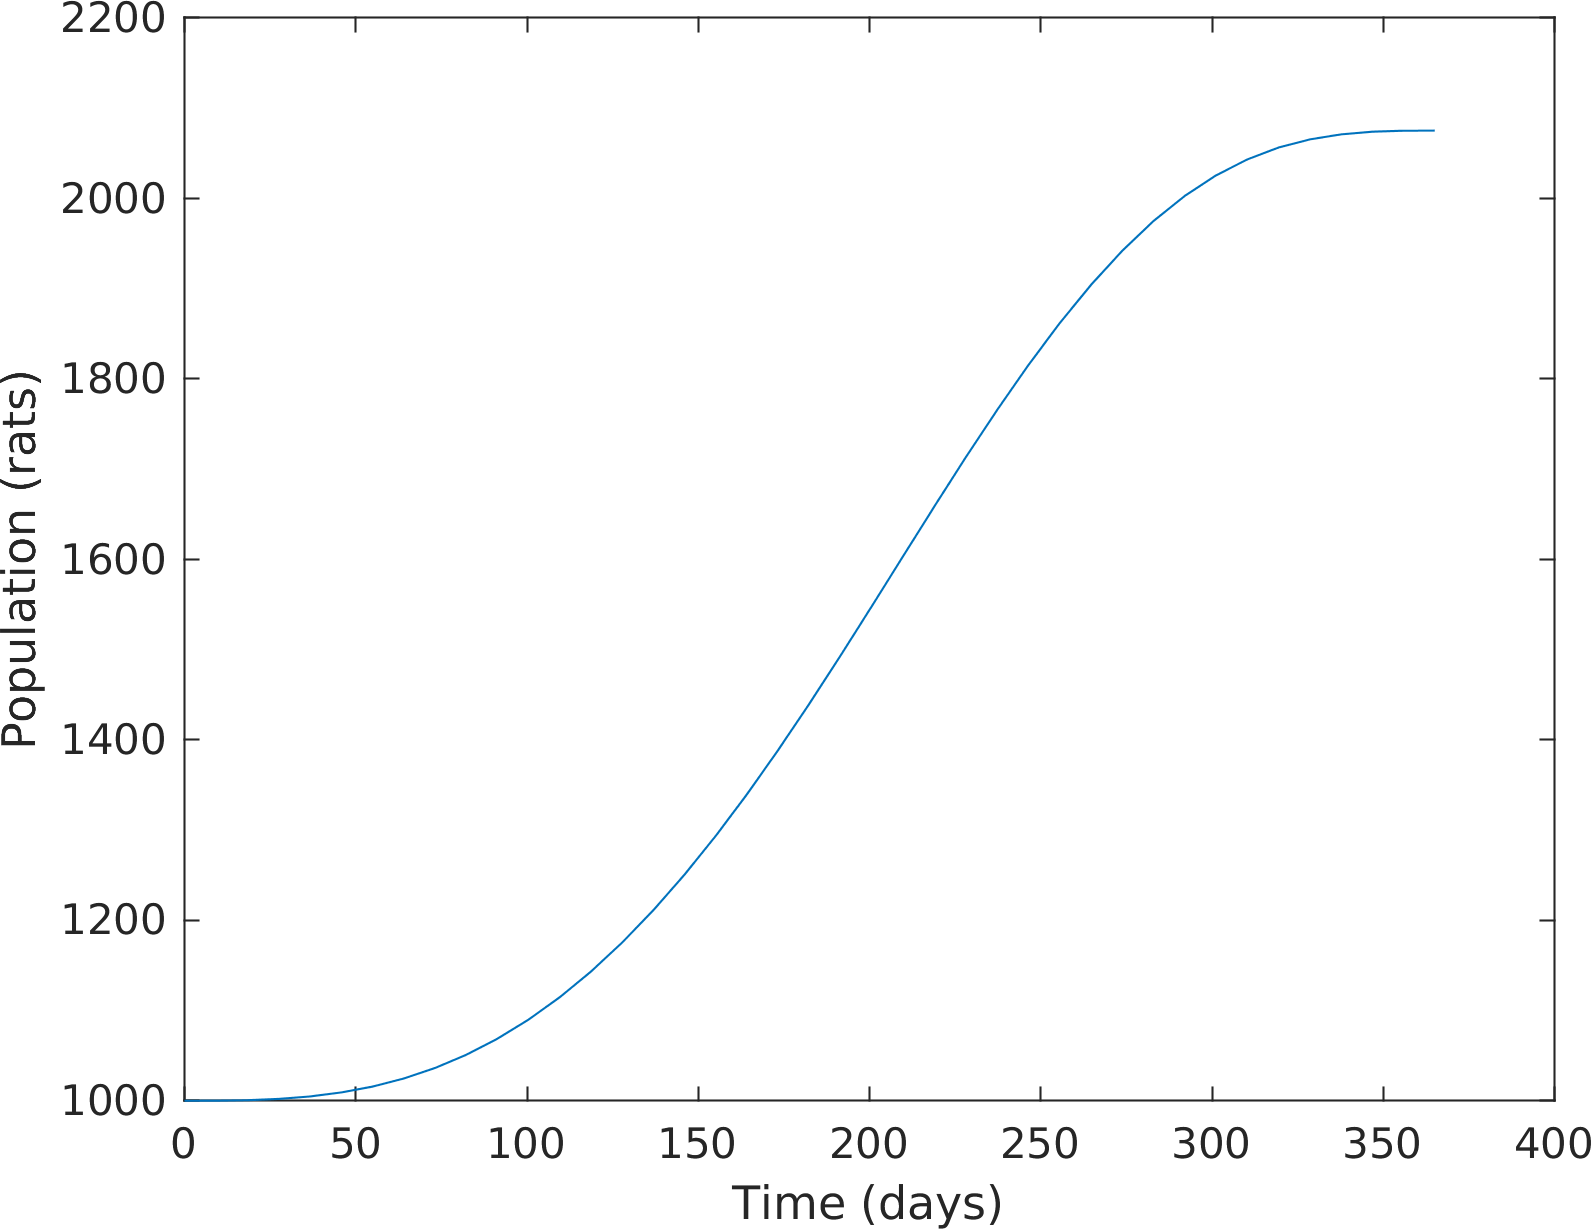
\includegraphics[width=0.7\textwidth]{w07_funcvectors_odes/lessons/rats.png}}
\caption{Solutions to a time-dependent differential equation by Euler's method and \lstinline{ode45}}
\label{fig:rats}
\end{figure}

The population grows slowly during the winter, quickly during the summer, and then slowly again in the fall.

To see the population at the end of the year, you can display the last element of \lstinline{rats}:

\begin{code}
rats(end)
2.0751e+03
\end{code}

That's a little more than 2000 rats, so the population roughly doubles in one year.

The index here is \lstinline{end}, which is a special word in MATLAB that means ``the index of the last element.''  You can use it in an expression, so \lstinline{Y(end - 1)} is the second-to-last element of
\lstinline{Y}.

\index{end statement@\lstinline{end} statement}
\index{index!end@\lstinline{end}}


\section{What Could Go Wrong?}

Don't forget the \lstinline{@} on the function handle.
If you leave it out, like:

\begin{code}
[tt, yy] = ode45(rate_func, [0, 365], 1000)
\end{code}
MATLAB treats the first argument as a function
call and calls \lstinline{rate_func} without providing arguments.
Then you get an error message:

\index{rate function}
\index{function handle}

\begin{code}
Not enough input arguments.

Error in rats>rate_func (line 18)
    res = a * y * (1 - cos(omega * t));

Error in rats (line 6)
    [tt, yy] = ode45(rate_func, [0, 365], 1000);
\end{code}

Also, the rate function you write has to take two input variables,
\lstinline{t} and \lstinline{y}, in that order, and return one output variable,
\lstinline{res}.

\index{output variable}

If you're working with a rate function like:

\begin{equation*}
\frac{dy}{dt}(t) = a y(t)
\end{equation*}
you might be tempted to write this:

\begin{code}
function res = rate_func(y)        % WRONG
    a = 0.002;
    res = a * y;
end
\end{code}

But that would be wrong.  So very wrong.  Why?  Because
when \lstinline{ode45} calls \lstinline{rate_func}, it provides two arguments.
If you only take one input variable, you'll get an error.  So
you have to write a function that takes \lstinline{t} as an input
variable, even if you don't use it:

\index{input variable}

\begin{code}
function res = rate_func(t, y)     % RIGHT
    a = 0.002;
    res = a * y;
end
\end{code}

Another common error is to write a function that doesn't make
an assignment to the output variable.  If you write something
like:

\begin{code}
function res = rate_func(t, y)
    a = 0.002;
    omega = 2*pi / 365;
    r = a * y * (1 - cos(omega * t));    % WRONG
end
\end{code}
 and then call it from \lstinline{ode45}, you get

\begin{code}
Output argument "res" (and maybe others) not assigned during call
to "rate_func".
\end{code}

I hope these warnings save you some time debugging.

\section{Labeling Axes}

The plots in this chapter have labels on the axes, and one of them has a legend, but I didn't show you how to do that.  Let's do it now.

\index{labeling axes}
\index{axes}
\index{xlabel@\lstinline{xlabel}}
\index{ylabel@\lstinline{ylabel}}

The functions to label the axes are \lstinline{xlabel} and \lstinline{ylabel}:

\begin{code}
xlabel('Time (hours)')
ylabel('Population (billions of cells)')
\end{code}

The function to generate a legend is \lstinline{legend}:

\begin{code}
legend('euler', 'ode45')
\end{code}

\index{legend@\lstinline{legend}}

The arguments are the labels for the lines, in the order they were drawn.  Usually the legend is in the upper-right corner, but you can move it by providing an optional argument called \lstinline{Location}:

\begin{code}
legend('euler', 'ode45', 'Location', 'northwest')
\end{code}

Finally,  save the figures using \lstinline{saveas}:

\begin{code}
saveas(gcf,'runge.png','png')
\end{code}

The first argument is the figure we want to save; \lstinline{gcf} is a MATLAB command that stands for ``get current figure,'' which is the figure we just drew.  The second argument is the filename.  The extension specifies the format we want, which is a PNG (\emph{.png}) image file.  The third argument tells MATLAB what driver to use.  The details aren't important, but \lstinline{'png'} generates figures as color images.

\index{figure}
\index{get current figure}
\index{gcf@\lstinline{gcf}}
\index{saveas@\lstinline{saveas}}


\section{How ode45 Works}
\label{s:howode45}

According to the MATLAB documentation, \lstinline{ode45} uses ``an explicit Runge-Kutta formula, the Dormand-Prince pair.''  You can read about it at  \url{https://greenteapress.com/matlab/runge}, but I'll give you a sense of it here.

\index{Runge-Kutta}
\index{ode45@\lstinline{ode45}}
\index{Dormand-Prince}

The key idea behind all Runge-Kutta methods is to evaluate the rate function several times at each time step and use a weighted average of the computed slopes to estimate the value at the next time step.
Different methods evaluate the rate function in different places and compute the average with different weights.

\index{differential equation}
\index{rate function}
\index{function!rate}

As an example, we'll solve the following differential equation:

\[ \frac{dy}{dt}(t) = y \sin t \]

Given a differential equation, it's usually straightforward to write a rate function:

\begin{code}
function res = rate_func(t, y)
    dydt = y * sin(t);
    res = dydt;
end
\end{code}

And we can use it like this:

\begin{code}
    y0 = 1;
    tspan=[0 4];
    options = odeset('Refine', 1);
    [T, Y] = ode45(@rate_func, tspan, y0, options);
\end{code}

For this example we'll use \lstinline{odeset} to set the \lstinline{Refine} option to \lstinline{1}, which tells \lstinline{ode45} to return only the time steps it computes, rather than interpolating between them.

\index{odeset@\lstinline{odeset}}

Now we can modify the rate function to plot the places where it gets evaluated:

\begin{code}
function res = rate_func(t, y)
    dydt = y * sin(t);
    res = dydt;

    plot(t, y, 'ro')
    dt = 0.01;
    ts = [t t+dt];
    ys = [y y+dydt*dt];
    plot(ts, ys, 'r-')
end
\end{code}

When \lstinline{rate_func} runs, it plots a red circle at each location and a short red line showing the computed slope.

\index{time step}

Figure~\ref{fig:odeplot1} shows the result;  \lstinline{ode45} computes 10 time steps (not counting the initial condition) and evaluates the rate function 61 times.

\begin{figure}[h]
\centerline{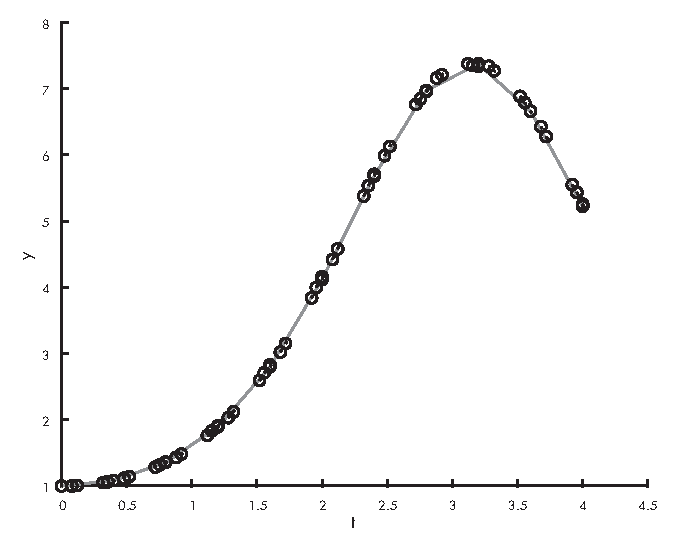
\includegraphics[scale=0.8]{images/figure15_01_new}}
\caption{Points where \lstinline{ode45} evaluates the rate function}
\label{fig:odeplot1}
\end{figure}

Figure~\ref{fig:odeplot2} shows the same plot, zoomed in on a single time step.
The dark squares at $0.8$ to $1.2$ show the values that were returned as part of the solution.
The circles show the places where the rate function was evaluated.

\begin{figure}[h]
\centerline{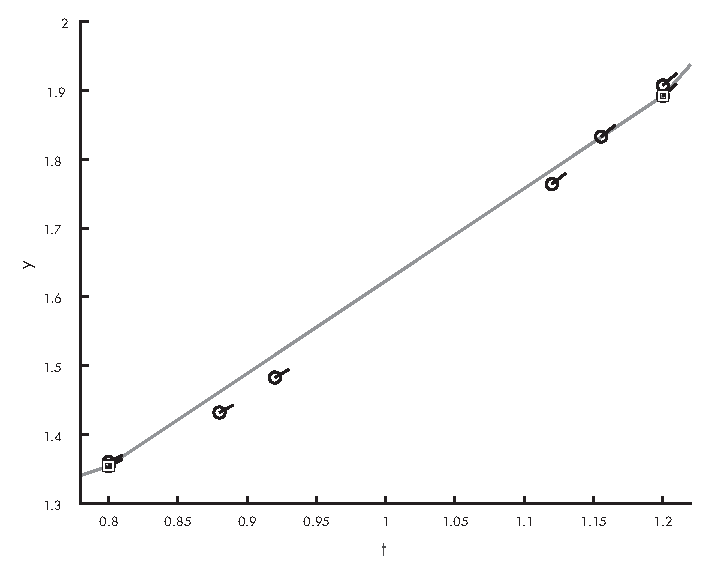
\includegraphics[scale=0.8]{images/figure15_02_new}}
\caption{Points where \lstinline{ode45} evaluates the rate function, zoomed in}
\label{fig:odeplot2}
\end{figure}

We can see that \lstinline{ode45} evaluates the rate function several times per time step, at several places between the end points.
We can also see that most of the places where \lstinline{ode45} evaluates the rate function are not part of the solution it returns, and they are not always good estimates of the solution.
This is good to know when you are writing a rate function; you should not assume that the time and state you get as input variables will be part of the solution.

In a sense, the rate function is answering a hypothetical question: ``\emph{If} the state at a particular time has these particular values, what \emph{would} the slope~be?''


At each time step, \lstinline{ode45} actually computes \emph{two} estimates of the next value.
By comparing them, it can estimate the magnitude of the error,  which it uses to adjust the time step.
If the error is too big, it uses a smaller time step; if the error is small enough, it uses a bigger time step.
Because \lstinline{ode45} is \emph{adaptive} in this way, it minimizes the number of times it calls the rate function to achieve a given level of accuracy.

\index{adaptive}



\section{Chapter Review}

This chapter introduced \emph{differential equations (DE)}, which are equations that describe the
derivatives of an unknown function.
In an \emph{ordinary differential equation (ODE)}, all derivatives are taken with
respect to the same variable, as opposed to a \emph{partial differential equation (PDE)}, which includes derivatives with respect to more than one variable.

A \emph{first-order DE} includes only first derivatives, and a \emph{linear DE} includes no products or powers of the function and its derivatives.
A differential equation is \emph{time dependent} if the rate function depends on time.

When we solve a differential equation numerically, the \emph{time step} is the interval in time between successive elements of the solution.
A \emph{parameter} is a value that appears in a model to quantify some
physical aspect of the scenario being modeled.

Until now, we have only put one function in each M-file, but in this chapter we wrote a \emph{main function}, which is the first function in an M-file, and a \emph{local function}, which is any function in an M-file that is not the main function.

In the next chapter, we'll solve \emph{systems} of ODEs, which are used to describe physical systems with multiple parts that interact.
But first, here's an exercise where you can apply what you've learned so far.


\section{Exercise}

Before you go on, you might want to work on the following exercise.

\begin{ex}

\index{coffee}
\index{cooling}
\index{Newton's law of cooling}

Suppose that you're given an 8-ounce cup of coffee at \SI{90}{\celsius}.
You have learned from bitter experience that the hottest coffee you
can drink comfortably is \SI{60}{\celsius}.

If the temperature of the coffee drops by \SI{0.7}{\celsius} during the first minute, how long will you have to wait to drink your coffee?

You can answer this question with Newton's Law of Cooling (see  \url{https://greenteapress.com/matlab/newton}):
%
\begin{equation*}
\frac{dy}{dt}(t) = -k (y(t) - e)
\end{equation*}
%
where $y(t)$ is the temperature of the coffee at time $t$,
$e$ is the temperature of the environment, and $k$ is a parameter
that characterizes the rate of heat transfer from the coffee to the environment.

Let's assume that $e$ is \SI{20}{\celsius} and constant; that is, the coffee does not warm up the room.

Let's also assume $k$ is constant.  In that case, we can estimate it based on the information we have.  If the temperature drops \SI{0.7}{\celsius} during the first minute, when the coffee is \SI{90}{\celsius}, we can write
%
\begin{equation*}
-0.7 = -k (90 - 20)
\end{equation*}
%

Solving this equation yields $k = 0.01$.

Here are some suggestions for getting started:

\begin{enumerate}

\item Create a file named \emph{coffee.m} and write a function
called \lstinline{coffee} that takes no input variables.  Put a simple statement like \lstinline{x = 5} in the body of the function and invoke \lstinline{coffee} from the Command  Window.

\item Add a helper function called \lstinline{rate_func} that takes \lstinline{t} and \lstinline{y} and computes $dy/dt$.  In this case, \lstinline{rate_func} does not actually depend on $t$; nevertheless, your function has to take $t$ as the first input variable in order to work with \lstinline{ode45}.

\item Test your function by adding a line like \lstinline{rate_func(0, 90)}
to \lstinline{coffee}, then call \lstinline{coffee} from the Command Window.
Confirm that the initial rate is \SI{-0.7}{\celsius \per \minute}.

\item Once you get \lstinline{rate_func} working, modify
\lstinline{coffee} to use \lstinline{ode45} to compute the temperature
of the coffee for 60 minutes.  Confirm that
the coffee cools quickly at first, then cools more slowly, and reaches
room temperature after about an hour.

\item Plot the results and estimate the time when the temperature reaches~\SI{60}{\celsius}.

\end{enumerate}

\end{ex}

\chapter{Matrices and Systems of ODEs}
\label{systems}


In the previous chapter we used Euler's method and \lstinline{ode45} to solve a single first-order differential equation.  In this chapter, we'll move on to systems of first-order ODEs and implement a model of a predator-prey system.  But first, we have to learn more about matrices.


\section{Matrices}

Recall from the introduction to Chapter~\ref{vectors} that the MATLAB's fundamental datatype is an array.  Scalars, in MATLAB, are actually 1-by-1 arrays with a single element and vectors are 1-by-N (or N-by-1) arrays with N elements.  We can even have empty arrays that have zero elements. We can demonstrate this by creating a few variables and interrogating the workspace using \lstinline{whos} to see how they are stored:

\begin{code}
     >> clear;
     w_empty = [];
     w_scalar = 1;
     x_scalar = [2];
     xx_vector = [1, 2, 3];
     whos
       Name           Size            Bytes  Class     Attributes
     
       w_empty        0x0                 0  double              
       w_scalar       1x1                 8  double              
       x_scalar       1x1                 8  double              
       xx_vector      1x3                24  double    
\end{code}

A \emph{matrix} is a two-dimensional array.  Like a vector,
it contains elements that are identified by indices.  The difference
is that the elements are arranged in rows and columns, so it takes
\emph{two} indices to identify an element.  Matrices are a powerful datatype because we can use tools from linear algebra to operate on matrices (and vectors).  

\subsection{Creating a Matrix}

\index{matrix}
\index{index}

A common way to create a matrix is the \lstinline{zeros} function,
which returns a matrix with the given size filled with zeros.
This example creates a matrix with two rows and three columns.

\begin{code}
>> M = zeros(2, 3)

M =  0     0     0
     0     0     0
\end{code}

If you don't know the size of a matrix, you can display it by using \lstinline{whos}:

\begin{code}
>> whos M
  Name      Size            Bytes  Class     Attributes
  M         2x3                48  double
\end{code}
or the \lstinline{size} function, which returns a vector:

\index{whos@\lstinline{whos}}
\index{size@\lstinline{size}}

\begin{code}
>> V = size(M)

V = 2    3
\end{code}

The first element is the number of rows; the second is the number of
columns.

\index{row}
\index{column}
\index{element}

To read an element of a matrix, you specify the row and column \mbox{numbers}:

\begin{code}
>> M(1,2)

ans = 0

>> M(2,3)

ans = 0
\end{code}

When you're working with matrices, it takes some effort to remember
which index comes first, row or column.  I find it useful to repeat
``row, column'' to myself, like a mantra.  You might also find it
helpful to remember ``down, across'' or the abbreviation RC as in ``radio control'' or RC Cola.

Another way to create a matrix is to enclose the elements in
brackets, with semicolons between rows:

\begin{code}
>> D = [1,2,3 ; 4,5,6]

D =  1     2     3
     4     5     6

>> size(D)

ans = 2     3
\end{code}

\index{semicolon}

\subsection{Row and Column Vectors}
\label{rowvector}

\index{row vectors}
\index{column vector}
\index{vector!row}
\index{vector!column}

Although it's useful to think in terms of numbers, vectors, and matrices,
from MATLAB's point of view everything is an array and MATLAB is particularly good and dealing with 2D arrays, matrices.  A number
is just a matrix that happens to have one row and one column:

\begin{code}
>> x = 5;
>> size(x)

ans = 1     1
\end{code}

And a vector is a matrix with only one row:

\begin{code}
>> R = 1:5;
>> size(R)

ans = 1     5
\end{code}

Well, some vectors have only one row, anyway.  Actually, there are two kinds
of vectors.  The ones we've seen so far are called \emph{row vectors},
because the elements are arranged in a row; the other kind are
\emph{column vectors}, where the elements are in a single column.

One way to create a column vector is to create a matrix with only
one element per row:

\begin{code}
>> C = [1;2;3]

C =

     1
     2
     3

>> size(C)

ans = 3     1
\end{code}

The difference between row and column vectors is important in
linear algebra, but for most basic vector operations, it doesn't matter.
For example, when you index the elements of a vector, you don't have to know what kind
it is:

\index{linear algebra}

\begin{code}
>> R(2)

ans = 2

>> C(2)

ans = 2
\end{code}


\subsection{The Transpose Operator}
\index{matrix transpose}

The transpose operator, which looks remarkably like an apostrophe,
computes the \emph{transpose} of a matrix, which is a new matrix
that has all the elements of the original, but with each row
transformed into a column (or you can think of it the other way around).

\index{transpose operator}

In this example \lstinline{D} has two rows:

\begin{code}
>> D = [1,2,3 ; 4,5,6]

D =  1     2     3
     4     5     6
\end{code}
so its transpose has two columns:

\begin{code}
>> Dt = D'

Dt = 1     4
     2     5
     3     6
\end{code}

\begin{ex}
What effect does the transpose operator
have on row vectors, column vectors, and numbers?
\end{ex}


\section{Solving Systems of ODEs}

Now that we've seen the basics of matrices, let's see how we can use them to solve systems of differential equations.

A generic form for a system of first-order, non-linear ODEs is the non-linear \emph{state-space} equation typically wrtiten as
\begin{equation} \label{e:nonlinearstatespace}
\dot{\mathbf{x}}(t) = \mathbf{f}(\mathbf{x}(t), \mathbf{u}(t))
\end{equation}
where \( \mathbf{x}(t) \) is the state vector, \( \mathbf{f} \) is a non-linear function of the state vector and \( \mathbf{u}(t) \) is the input vector.  We've used the notation convention where scalar variables are expressed in regular font (e.g., $t$), vectors are in bold font (e.g., $\mathbf{x}$) and matrices are capitalized (e.g., $A$).  If we can get our problem into this form, we can then apply a variety of MATLAB numerical tools to solve the system of equations.

\subsection{Lotka-Volterra}
\label{lotka}

The Lotka-Volterra model describes the interactions between two
species in an ecosystem, a predator and its prey.  As an example, we'll consider foxes and rabbits.

\index{Lotka-Volterra model}
\index{rabbit}
\index{fox}
\index{system!of ODEs}

The model is governed by the following system of first-order, non-linear differential equations:

\begin{eqnarray*}
    \frac{dx}{dt} &=& a x - b x y         \\
    \frac{dy}{dt} &=& -c y + d x y
\end{eqnarray*}
%
where $x$ and $y$ are the populations of rabbits and foxes,
and $a$, $b$, $c$, and $d$ are parameters
that quantify the interactions between the two species (see
\url{https://greenteapress.com/matlab/lotka}).

We can put this model into the state-space form of Equation~\ref{e:nonlinearstatespace}.  The first step is to define the state as the vector of rabbits and foxes,
\begin{equation*}
\dot{\mathbf{x}}(t)  = \left\{ \begin{array}{c}
     x(t) \\
     y(t)
\end{array}\right\}.
\end{equation*}
Using this state, the right side of our model is only a function of those state values---there is no external input.  So there is no input vector $\mathbf{u}(t)$.  So in standard state-space form our model is
\begin{equation*}
     \left\{ \begin{array}{c}
          \dot{x}(t) \\
          \dot{y}(t)
     \end{array}\right\} = 
     \left[  \begin{array}{c}
          ax - bxy \\
          -cy + dxy
     \end{array}\right].
     \end{equation*}

At first glance, you might think you could solve these equations by
calling \lstinline{ode45} once to solve for $x$ and
once to solve for $y$.  The problem is that each equation involves
both variables, which is what makes this a \emph{system of equations}
and not just a list of unrelated equations.  To solve a system, you
have  to solve the equations simultaneously.

\index{system!of equations}
\index{ode45@\lstinline{ode45}}

Fortunately, \lstinline{ode45} can handle systems of equations.  The
difference is that the initial condition is a vector that contains the
initial values $x(0)$ and $y(0)$, and the output is a matrix
that contains one column for $x$ and one for $y$.

\index{rate function}

Listing~\ref{lst:lotka_volterra} shows the rate function
with the parameters $a = 0.1$, $b = 0.01$, $c = 0.1$, and $d = 0.002$:

\begin{lstlisting}[caption={A rate function for Lotka-Volterra}, label={lst:lotka_volterra}]
function res = rate_func(t, V)
    % unpack the elements of V
    x = V(1);
    y = V(2);

    % set the parameters
    a = 0.1;
    b = 0.01;
    c = 0.1;
    d = 0.002;

    % compute the derivatives
    dxdt = a*x - b*x*y;
    dydt = -c*y + d*x*y;

    % pack the derivatives into a column vector
    res = [dxdt; dydt];
end
\end{lstlisting}

The first input variable, \lstinline{t}, is time.
Even though the time variable is not used in this rate function,
it has to be there in order for this function to work with \lstinline{ode45}.
The second input variable, \lstinline{V}, is a vector with two elements,
$x(t)$ and $y(t)$.
The body of the function includes four sections, each explained by a comment.

The first section \emph{unpacks} the vector by copying the elements
into variables.  This isn't necessary, but giving names to
these values will help you to remember what's what.  It also makes the third
section, where we compute the derivatives, resemble the mathematical
equations we were given, which helps prevent errors.

\index{pack vector}
\index{unpack vector}

The second section sets the parameters that describe the
reproductive rates of rabbits and foxes, and the characteristics of
their interactions.  If we were studying a real system, these values
would come from observations of real animals, but for this example
I chose values that yield interesting results.

\index{parameter}

The third section computes the derivatives of $x$ and $y$, using the equations
we were given.

The last section \emph{packs} the computed derivatives back into a
vector.  When \lstinline{ode45} calls this function, it provides a vector
as input and expects to get a vector as output.

Sharp-eyed readers will notice something different about this line:

\begin{code}
    res = [drdt; dfdt];
\end{code}

The semicolon between the elements of the vector is not an error.  It
is necessary in this case because \lstinline{ode45} requires the result of
this function to be a column vector.

\index{semicolon}

As always, it's a good idea to test your rate function before you call \lstinline{ode45}.
Create a file named \emph{lotka.m} with the following main function:

\begin{code}
function res = lotka()
    t = 0;
    V_init = [80, 20];
    rate_func(t, V_init)
end
\end{code}

\index{initial condition}

\lstinline{V_init} is a vector that represents the initial condition, 80 rabbits and 20 foxes.
The result from \lstinline{rate_func} is

\begin{code}
-8.0000
 1.2000
 \end{code}
which means that with these initial conditions, we expect the rabbit population to decline initially at a rate of 8 per week and the fox population to increase by 1.2 per week.

Now we can run \lstinline{ode45} like this:

\begin{code}
tspan = [0, 200]
[T, M] = ode45(@rate_func, tspan, V_init)
\end{code}

The first argument is the function handle for the rate function.
The second argument is the time span, from 0 to 200 weeks.
The third argument is the initial condition.

\index{function handle}
\index{handle!function}


\subsection{Output Matrices}

The \lstinline{ode45} function returns two values: \lstinline{T}, a vector,
and \lstinline{M}, a matrix.

\begin{code}
>> size(T)
ans = 101     1

>> size(M)
ans = 101     2
\end{code}

\lstinline{T} has 101 rows and 1 column, so it is a column vector with one row for
each time step.

\lstinline{M} has 101 rows, one for each time step, and 2 columns, one for each variable,
$x$ and $y$.

This structure---one column per variable---is a common way to
use matrices. And \lstinline{plot} understands this structure, so if you
do the following:

\begin{code}
>> plot(T, M)
\end{code}
MATLAB understands that it should plot each column from \lstinline{M}
versus \lstinline{T}.

\index{colon}

You can copy the columns of \lstinline{M} into other variables like
this:

\begin{code}
>> R = M(:, 1);
>> F = M(:, 2);
\end{code}

In this context, the colon represents the range from \lstinline{1} to \lstinline{end},
so \lstinline{M(:, 1)} means ``all the rows, column 1'' and
\lstinline{M(:, 2)} means ``all the rows, column 2.''

\begin{code}
>> size(R)
ans = 101     1

>> size(F)
ans = 101     1
\end{code}

So \lstinline{R} and \lstinline{F} are column vectors.

\index{column vector}

Now we can plot these vectors separately, which makes it easier to give them different style strings:

\begin{code}
>> plot(T, R, '-')
>> plot(T, F, '--')
\end{code}


Figure~\ref{fig:lotka} shows the results. The x-axis is time in weeks; the y-axis is population.  The top curve shows the population of rabbits; the bottom curve shows foxes.

\begin{figure}[h]
\centerline{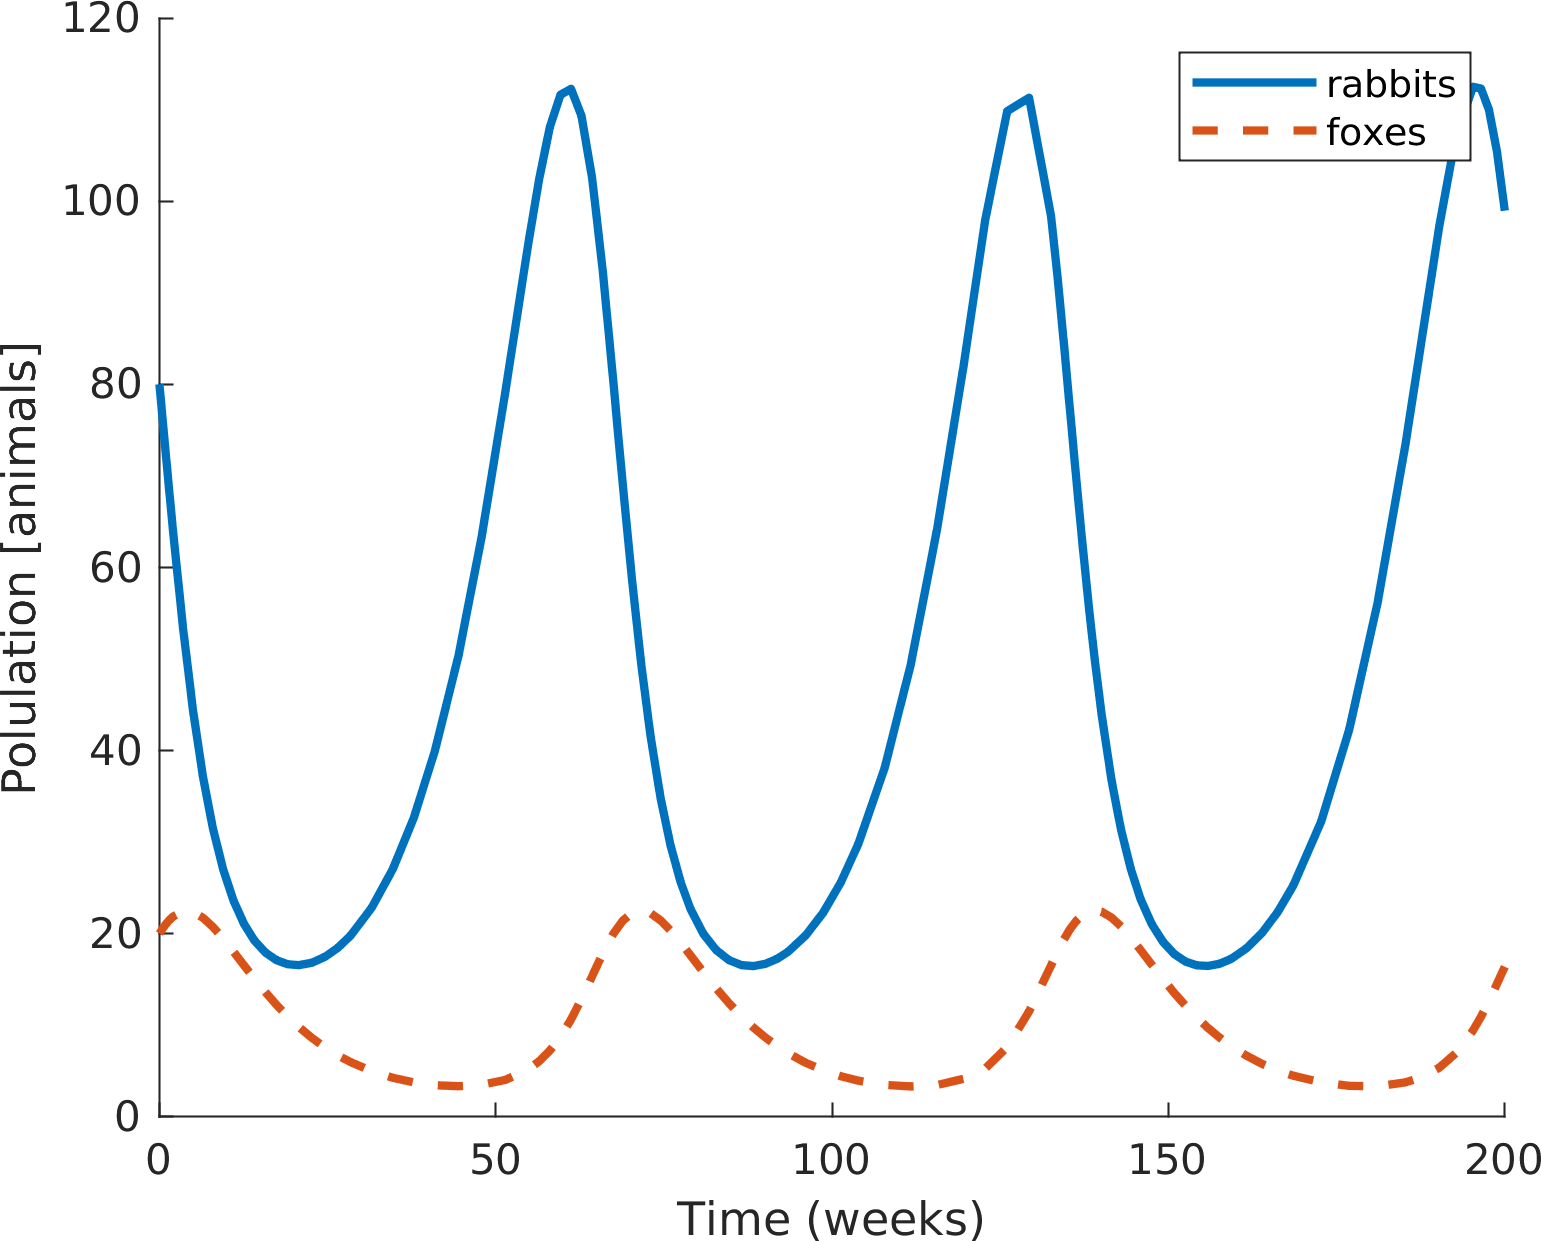
\includegraphics[width=0.7\textwidth]{w08_matrices_secondorder/lessons/lotka_time.png}}
\caption{Solution for the Lotka-Volterra model}
\label{fig:lotka}
\end{figure}

\index{boom and bust}

Initially, there are too many foxes, so the rabbit population declines.  Then there are not enough rabbits, and the fox population declines.  That allows the rabbit population to recover, and the pattern repeats.

This cycle of ``boom and bust'' is typical of the Lotka-Volterra model.


\subsection{Phase Plot}

Instead of plotting the two populations over time, it is sometimes useful to plot them against each other:

\begin{code}
>> plot(R, F)
\end{code}

Figure~\ref{fig:phase} shows the result, which is called a \emph{phase plot}.
Each point on this plot represents a certain number of rabbits (on the
x-axis) and a certain number of foxes (on the y-axis).
Since these are the only two variables in the system, each point in
this plane describes the complete \emph{state} of the system, that is, the values of
the variables we're solving for.

\begin{figure}[ht]
\centerline{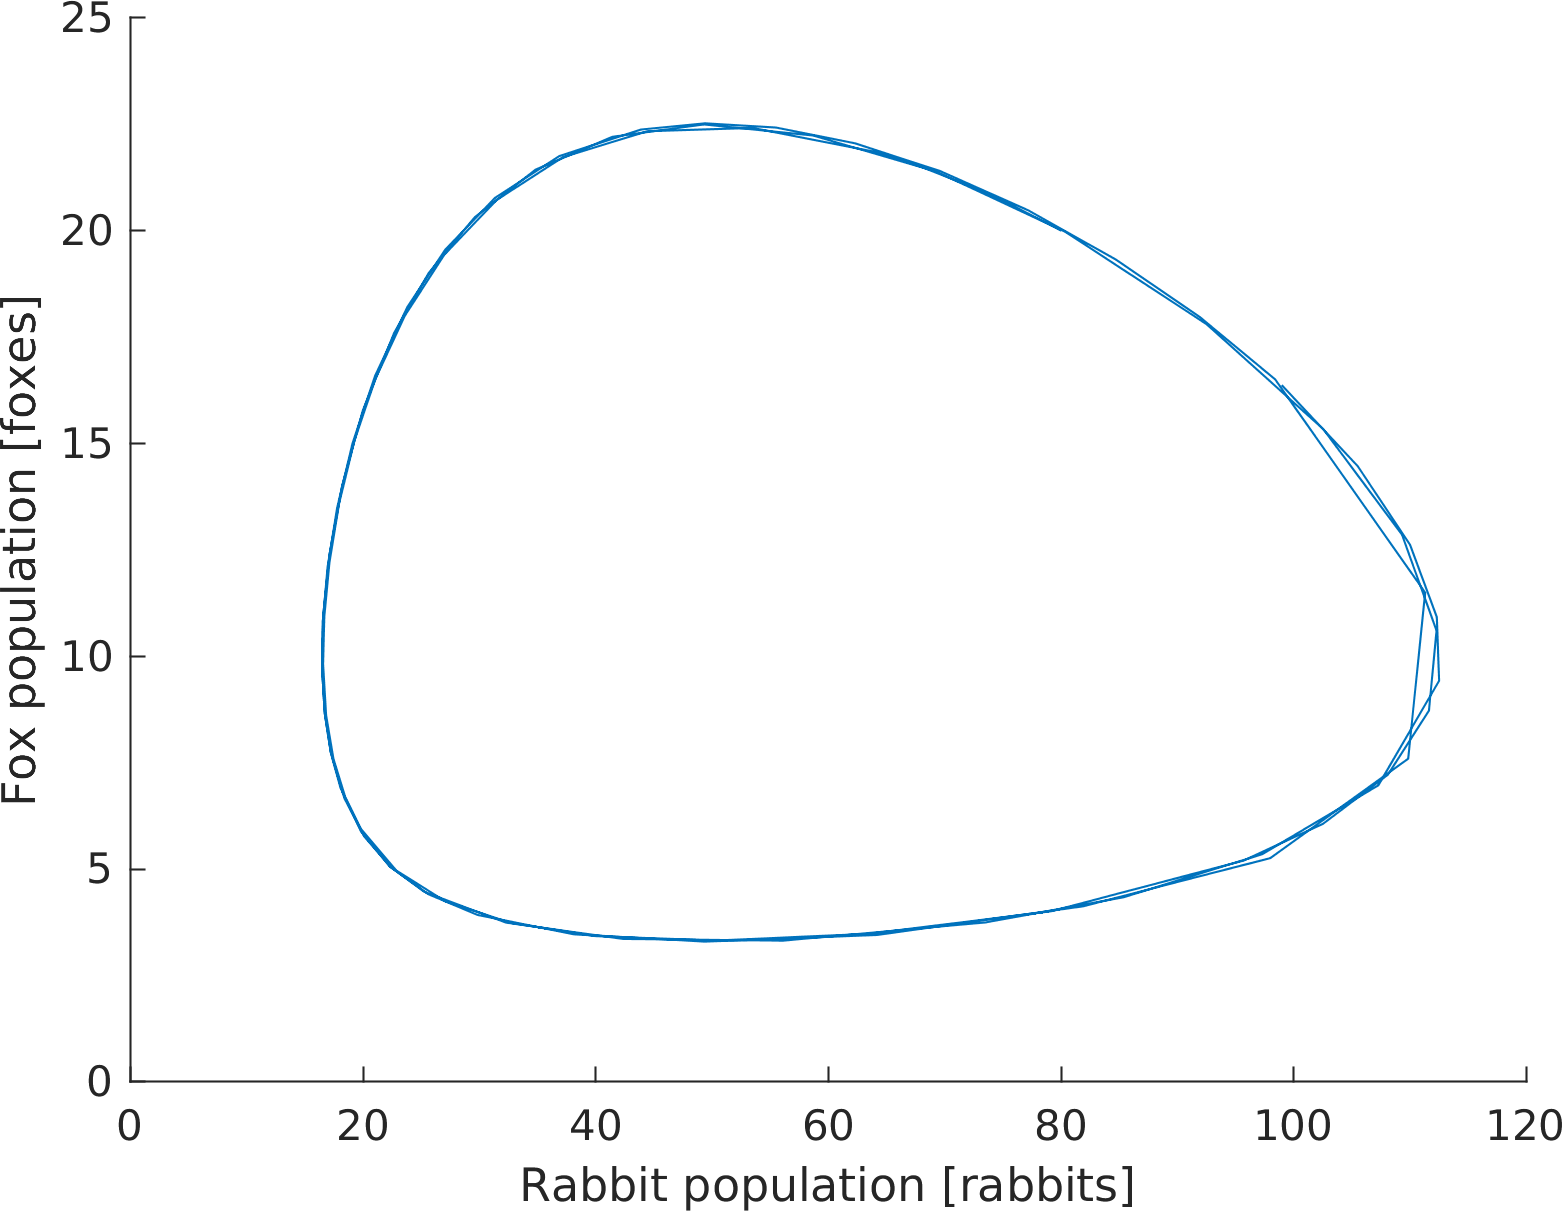
\includegraphics[width=0.7\textwidth]{w08_matrices_secondorder/lessons/lotka_state.png}}
\caption{Phase plot from the Lotka-Volterra model}
\label{fig:phase}
\end{figure}

\index{phase plot}
\index{trajectory}
\index{state}

Over time, the state moves around the plane. Figure~\ref{fig:phase} shows
the path traced by the state over time; this path
is called a \emph{trajectory}.

Since the behavior of this system is periodic, the trajectory is a loop.

If there are three variables in the system, we need three dimensions to show
the state of the system, so the trajectory is a 3D curve.
You can use \lstinline{plot3} to trace trajectories in three dimensions,
but for four or more variables, you're on your own.

\index{plot3@\lstinline{plot3}}


\subsection{What Could Go Wrong?}

The output vector from the rate function has to be a column vector, otherwise you get an error:

\begin{code}
Error using odearguments (line 93)
RATE_FUNC must return a column vector.
\end{code}
which is a pretty good error message.  It's not clear \emph{why}
it needs to be a column vector, but that's not our problem.

\index{column vector}

Another possible error is reversing the order of the elements in the
initial conditions or the vectors inside \lstinline{lotka}.  MATLAB
doesn't know what the elements are supposed to mean, so it can't catch
errors like this; it will just produce incorrect results.

The order of the elements (rabbits and foxes) is up to you, but
you have to be consistent.  That is, the order of the initial conditions you
provide when you call \lstinline{ode45} has to be the same as the order
inside \lstinline{rate_func} where you unpack the input vector and the
same as the order of the derivatives in the output vector.

\section{Chapter Review}

In this chapter, we used \lstinline{ode45} to solve a system of first-order differential equations.
As an exercise, you'll have a chance to solve the famous Lorenz equations, one of the first examples of a chaotic system.

Here are the terms from this chapter you might want to remember.

A \emph{row vector} is a matrix that has only one row, and a \emph{column vector} is a matrix that has only one column.
The \emph{transpose operation} transforms the  rows of a matrix
into columns (or the other way around, if you prefer).

A \emph{system of equations} is a collection of equations written in terms of
the same set of variables.

In a rate function, we often have to \emph{unpack} the input variable,
copying the elements of a vector into a set of variables.
Then we have to \emph{pack} the results into a vector as an output variable.

The \emph{state} of a system is a set of variables that quantify the condition of the system as it changes over time.

When we solve a system of differential equations, we can visualize the results with a \emph{phase plot}, which shows the state of a system as a point in the space of possible states.
A \emph{trajectory} is a path in a phase plot that shows how the state of a system changes over time.

In the next chapter, we'll move on to second-order systems, which we use to describe systems
with objects moving in space, governed by Newton's laws of motion.


\section{Exercises}

Before you go on, you might want to work on the following exercise.

\begin{ex}

\index{Lorenz attractor}

Based on the examples we've seen so far, you'd think that all ODEs describe population as
a function of time, but that's not true.

For example, the Lorenz system is a system of differential equations based on a model of fluid dynamics in the atmosphere
(see \url{https://greenteapress.com/matlab/lorenz}).
It turns out to be interesting in part because its solutions are chaotic; that is, small changes in the initial conditions yield big differences in the solutions.

The system is described by these differential equations:
%
\begin{eqnarray*}
x_t &=& \sigma (y - x)  \\
y_t &=& x (r - z) - y   \\
z_t &=& xy - b z
\end{eqnarray*}
%
Common values for the parameters are $\sigma = 10$, $b = 8/3$, and $r=28$.

Use \lstinline{ode45} to estimate a solution to this system of equations.

\begin{enumerate}

\item Create a file named \emph{lorenz.m} with a main function named \lstinline{lorenz} and a helper function named \lstinline{rate_func}.

\item  The rate function should
take \lstinline{t} and \lstinline{V} as input variables, where the components
of \lstinline{V} are understood to be the current values of \lstinline{x},
\lstinline{y}, and \lstinline{z}.  It should compute the corresponding derivatives
and return them in a single column vector.

\item Test the function by calling it from the main function with values like $t=0$, $x=1$, $y=2$, and $z=3$.
Once you get your function working, you should make it a silent function before calling \lstinline{ode45}.

\item Use \lstinline{ode45} to estimate the solution for the time span $[0, 30]$
with the initial condition $x=1$, $y=2$, and $z=3$.

\item Plot the results as a time series, that is, each of the variables as a function of time.

\item Use \lstinline{plot3} to plot the trajectory of $x$, $y$, and $z$.

\end{enumerate}

% lorenz.m

\end{ex}

\chapter{Second-Order Systems}


So far we've seen first-order differential equations and systems of first-order ODEs.  In this chapter, we'll introduce second-order systems, which are particularly useful for modeling Newtonian motion.

\index{Newtonian motion}
\index{Newton's law of motion}

\section{Newtonian Motion}
\label{s:newton}

Newton's second law of motion is often written like this:

\begin{equation*}
    F = m a
\end{equation*}
where $F$ is the net force acting on an object, $m$ is the
mass of the object, and $a$ is the acceleration of the object.

This equation suggests
that if you know $m$ and $a$, you can compute the force. And that's true,
but in most physical simulations it's the other way around: based on a
physical model, you know $F$ and $m$, and you compute $a$.

\index{second derivative}
\index{second-order differential equation}
\index{differential equation!second-order}

So if we know acceleration as a function of time, how do we
find the position of the object, $r$?  Well, we know that acceleration
is the second derivative of position, so we can write the differential
equation

\begin{equation*}
    \frac{d^2r}{dt^2} = a
\end{equation*}
where ${d^2r}/{dt^2}$ is the second time derivative of $r$.

Because this equation includes a second derivative, it's
a second-order ODE.  We can't solve the equation using \lstinline{ode45} in this form, but
by introducing a new variable, \emph{v}, for velocity, we can rewrite it
as a system of first-order ODEs:

\begin{eqnarray*}
    \frac{dr}{dt} &=& v   \\
    \frac{dv}{dt} &=& a
\end{eqnarray*}

The first equation says that the first derivative of $r$ is $v$;
the second equation says that the first derivative of $v$ is $a$.

Another way to present this model is to put it into linear \emph{state space} form.  The standard form for the state equation is
\begin{equation} \label{e:statespace}
    \dot{\mathbf{x}}(t) = A \mathbf{x}(t) + B \mathbf{u}(t) 
\end{equation}
where $\mathbf{x}(t)$ is the state vector of the system, $\mathbf{u}(t)$ is the input vector to the system, $A$ is the state transition matrix and $B$ is the input matrix.  Again we've used the notation convention where scalar variables are expressed in regular font (e.g., $t$), vectors are in bold font (e.g., $\mathbf{x}$) and matrices are capitalized (e.g., $A$).  This linear form is a special case of the more general non-linear state-space form in Equation~\ref{e:nonlinearstatespace}

To get our system of equations into state space form we can define the state vector as a column vector with elements of position ($r(t)$) and velocity ($v(t)$).

\begin{equation}
\left\lbrace
\begin{array}{c}
    \dot{r}(t) \\
    \dot{v}(t)
\end{array}
\right\rbrace
=
\left[ \begin{array}{cc}
0 & 1 \\
0 & 0 
\end{array} \right]
\left\{ \begin{array}{c}
    r(t) \\ v(t)
\end{array} \right\}
+ 
\left[ \begin{array}{c}
    0 \\ 1
\end{array} \right]
\left\{ a \right\}
\end{equation}

It turns out that any higher-order ordinary differential equation (ODE) can be transformed into a system of first-order ODEs. Numerical methods, such as \lstinline{ode45} are often setup to operate on these systems of first-order ODEs.  This example, of transforming a single second-order ODE into a system of two first-order ODEs is a specific example of a general approach.

\section{Free Fall}
\label{freefall}

As an example of Newtonian motion, let's go back to the question from Section~\ref{penny}:

\begin{quote}
If you drop a penny from the top of the Empire State Building, how long does it take to reach the sidewalk, and how fast is it going when it gets there?
\end{quote}

We'll start with no air resistance; then we'll add air resistance to the model and see what effect it has.

\index{air resistance}
\index{gravity}

Near the surface of the earth,
acceleration due to gravity is \SI{-9.81}{\meter \per \second \squared}, where the minus sign
indicates that gravity pulls down, so $a=\SI{-9.81}{m/s^2}$.
If the object falls straight down, we can describe its position with a
scalar value $y$, representing altitude.

\index{position}
\index{velocity}
\index{rate function}
Listing~\ref{lst:penny_rate_func} contains a rate function we can use with \lstinline{ode45} to solve
this problem:

\begin{lstlisting}[caption={A rate function for the falling penny problem}, label={lst:penny_rate_func}]
function xx_dot = rate_func(t, xx)
    % Rate function using state space format
    A = [0, 1; 0, 0];
    B = [0; 1];
    uu = -9.81;
    
    xx_dot = A*xx+B*uu;
end
\end{lstlisting}

The rate function in Listing~\ref{lst:penny_rate_func} takes scalar \lstinline{t} and column vector \lstinline{xx} as input variables, where the elements of \lstinline{xx} are understood to be the position and velocity of the penny.

It returns a column vector that contains which are velocity and acceleration, respectively.

As always, we should test the rate function before we call \lstinline{ode45}.  Here's the top-level function we can use to test it:

\begin{code}
% Initial conditions as state vector: position and velocity
xx_init = [381; 0];

% Test the rate function
rate_func(0, xx_init)
\end{code}

The initial condition of \lstinline{xx} is the initial position, which is the height of the Empire State Building, about \SI{381}{\meter}, and the initial velocity, which is \SI{0}{\meter \per \second}.

\index{Empire State Building}
\index{penny}

The result from \lstinline{rate_func} is

\begin{code}
    0
   -9.8000
\end{code}
which is what we expect.

Now we can run \lstinline{ode45} with this rate function:

\begin{code}
tspan = [0, 10]
[tout, Xout] = ode45(@rate_func, tspan, xx_init);
\end{code}

As always, the first argument is the function handle, the second is the time span (10 seconds), and the third is the initial condition.

The result is a vector, \lstinline{tout}, that contains the time values, and a matrix, \lstinline{Xout}, that contains two columns, one for altitude and one for velocity.
\index{function handle}
\index{time span}
\index{matrix}

We can extract the first column and plot it, like this:

\begin{code}
Y = Xout(:, 1)
plot(T, Y)
\end{code}

Here is the full listing\dots
\lstinputlisting[style=mcode]{w08_matrices_secondorder/lessons/penny1.m}

\begin{figure}
\centerline{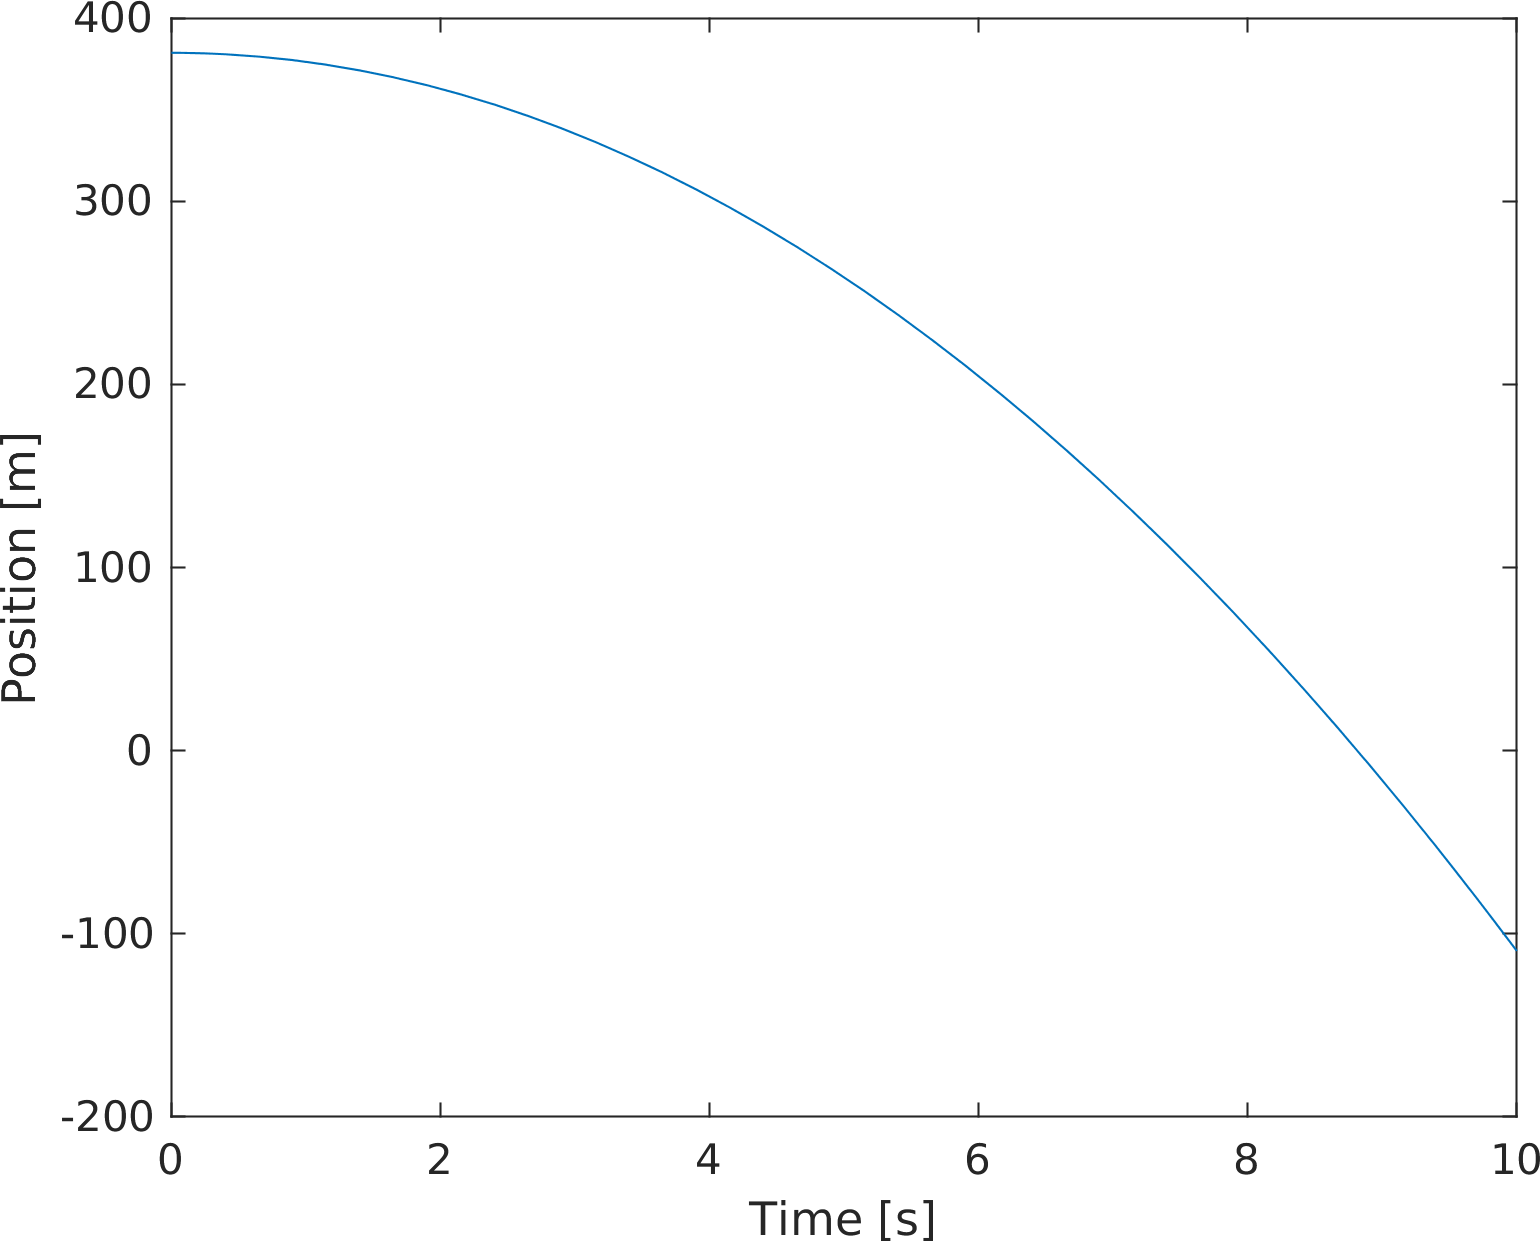
\includegraphics[width=0.7\textwidth]{w08_matrices_secondorder/lessons/penny1.png}}
\caption{Altitude versus time for an object in free fall}
\label{fig:penny}
\end{figure}

Figure~\ref{fig:penny} shows the result.  Altitude drops slowly at first and picks up speed.  Between 8 and 9 seconds, the altitude reaches 0, which means the penny hits the sidewalk.  But \lstinline{ode45} doesn't know where the ground is, so  the penny keeps going through 0 into negative altitude.  We'll solve that problem in the next section.

\section{ODE Events}
\label{events}

\index{ODE event}

Normally when you call \lstinline{ode45} you specify a start time and
an end time.  But sometimes you don't know ahead of time when the
simulation should end.  To solve this problem we can define an \emph{event},
something of interest that happens during a simulation,
like the penny reaching the ground.

Here are the steps:

\index{event function}
\index{function!event}
\index{ODE event}

\begin{enumerate}

\item First we define an \href{https://www.mathworks.com/help/matlab/math/ode-event-location.html}{\emph{event function}} that allows \lstinline{ode45} to figure out when
an event occurs.  Here's an event function for the penny example:

\begin{code}
function [value, isterminal, direction] = event_func(t,xx)
    value = xx(1);
    isterminal = 1;
    direction = -1;
end
\end{code}

The event function takes the same input variables as the rate function and returns three output variables: \lstinline{value} is zero when an event can occur, \lstinline{direction} can be 0 to allow all events, +1 for the event to occur only when the event function is increasing, and \lstinline{isterminal} is 1 if the integration should terminate and 0 otherwise. 
More specifically, an event can occur when \lstinline{value} passes through 0.
If \lstinline{direction} is positive, the event only occurs if \lstinline{value} is increasing.
 If \lstinline{direction} is negative, the event only occurs if \lstinline{value} is decreasing.
If \lstinline{direction} is 0, the event always occurs.
If \lstinline{isterminal} is 1, the event causes the simulation to end; if it is 0, the simulation continues.

This event function uses the altitude of the penny as \lstinline{value} so an event can occur when altitude passes through 0.
Because \lstinline{direction} is negative, an event occurs only when altitude is decreasing, and
because \lstinline{isterminal} is 1, the simulation ends if an event occurs.

\index{odeset@\lstinline{odeset}}
\index{options@\lstinline{options}}

\item Next, we use \lstinline{odeset} to create an object called \lstinline{options}:

\begin{code}
options = odeset('Events', @event_func);
\end{code}
%
The name of the option is \lstinline{Events} and the value is the handle of the event function.

\item Finally, we pass \lstinline{options} as a fourth argument to \lstinline{ode45}:

\begin{code}
[tout, Xout] = ode45(@rate_func, tspan, xx_init, options);
\end{code}

When \lstinline{ode45} runs, it invokes \lstinline{event_func} after each time step.  If the event function indicates that a terminal event occurred,
\lstinline{ode45} stops the simulation.

\end{enumerate}

Let's look at the results from the penny example:

\begin{code}
    >> tout(end)
    ans =
    8.8134
    
    >> Xout(end,:)
    ans =
             0  -86.4594
\end{code}

The last value of \lstinline{tt} is about 8.8, which is the number of seconds the penny takes to reach the sidewalk.

The last row of \lstinline{Xout} indicates that the final altitude is 0, which is what we wanted, and the final velocity is about \SI{-86}{\meter \per \second}.


\section{Air Resistance}
\label{air_resistance}

\index{drag}
\index{air resistance}

To make this simulation more realistic, we can add air resistance.
For large objects moving quickly through air, the force due to air resistance, \emph{drag}, is proportional to velocity squared.
For an object falling down, drag is
directed up, so if velocity is negative, drag force is positive.

% b is used in the book "Physics for Scientists and Engineers" by Paul A. Tipler.
%TODO: consider writing out the drag equation

Here's how we can compute the force of drag as a function of velocity in one dimension:

\begin{equation*}
    f_\mathrm{d} = -\mathrm{sign}(v) b v^2
\end{equation*}
where $v$ is velocity and
$b$ is a drag constant that depends on the density of
air, the cross-sectional area of the object, and the shape
of the object.

The sign or signum function returns the value $1$ for positive values of
$v$ and $-1$ for negative values.  So $f_\mathrm{d}$ is always in the opposite direction of $v$.

\index{signum function}
\index{sign@\lstinline{sign}}
\index{mass}
\index{terminal velocity}

To convert from force to acceleration we have to know mass, but that's easy to find: the mass of a penny is about \SI{2.5}{\gram}.  It's not as easy to find the drag constant, but based on reports that the terminal velocity of a penny is about \SI{18}{\meter \per \second}, I've estimated that it's about \SI{75e-6}{\kilogram \per \meter}.

Listing~\ref{lst:acceleration_drag} defines a function that takes \lstinline{t} and \lstinline{X} as input variables and returns the total acceleration of the penny due to gravity and drag:

\begin{lstlisting}[caption={Calculating acceleration of a penny with drag}, label={lst:acceleration_drag}]
function accel = acceleration(t, xx)
    % Return total acceleration due to gravity and drag.
    
    % Drag constant in kg/m
    b = 75e-6; 
    % Velocity from state, in m/s
    v = xx(2);
    % Drag force in N    
    f_d = -sign(v) * b * v^2;
    % Mass in kg
    m = 2.5e-3;
    % Drag acceleration in m/s^2
    a_d = f_d / m;
    % Gravity
    a_g = -9.8;
    % Return total drag
    accel = a_g + a_d;
end
\end{lstlisting}

First, we compute force due to drag. Then we compute acceleration due to drag. Lastly, we compute total acceleration due to drag and gravity.

\index{acceleration}
\index{force}

Be careful when you're working with forces and accelerations; make sure
you only add forces to forces or accelerations to accelerations.  In my
code, I use comments to remind myself what units the values have.
That helps me avoid errors like adding forces to accelerations.

To use this function, we make a small change in \lstinline{rate_func}:

\begin{code}
function xx_dot = rate_func(t, xx)
    % Rate function using state space format
    A = [0, 1; 0, 0];
    B = [0; 1];
    % Intput is total acceleration - this line has changed!
    uu = acceleration(t, xx);
    
    xx_dot = A*xx+B*uu;
end
\end{code}

In the previous version, acceleration is always \lstinline{-9.8}, the acceleration due to gravity.
In this version, we call \lstinline{acceleration} to compute the total acceleration due to gravity and drag.

\begin{figure}[ht]
\centerline{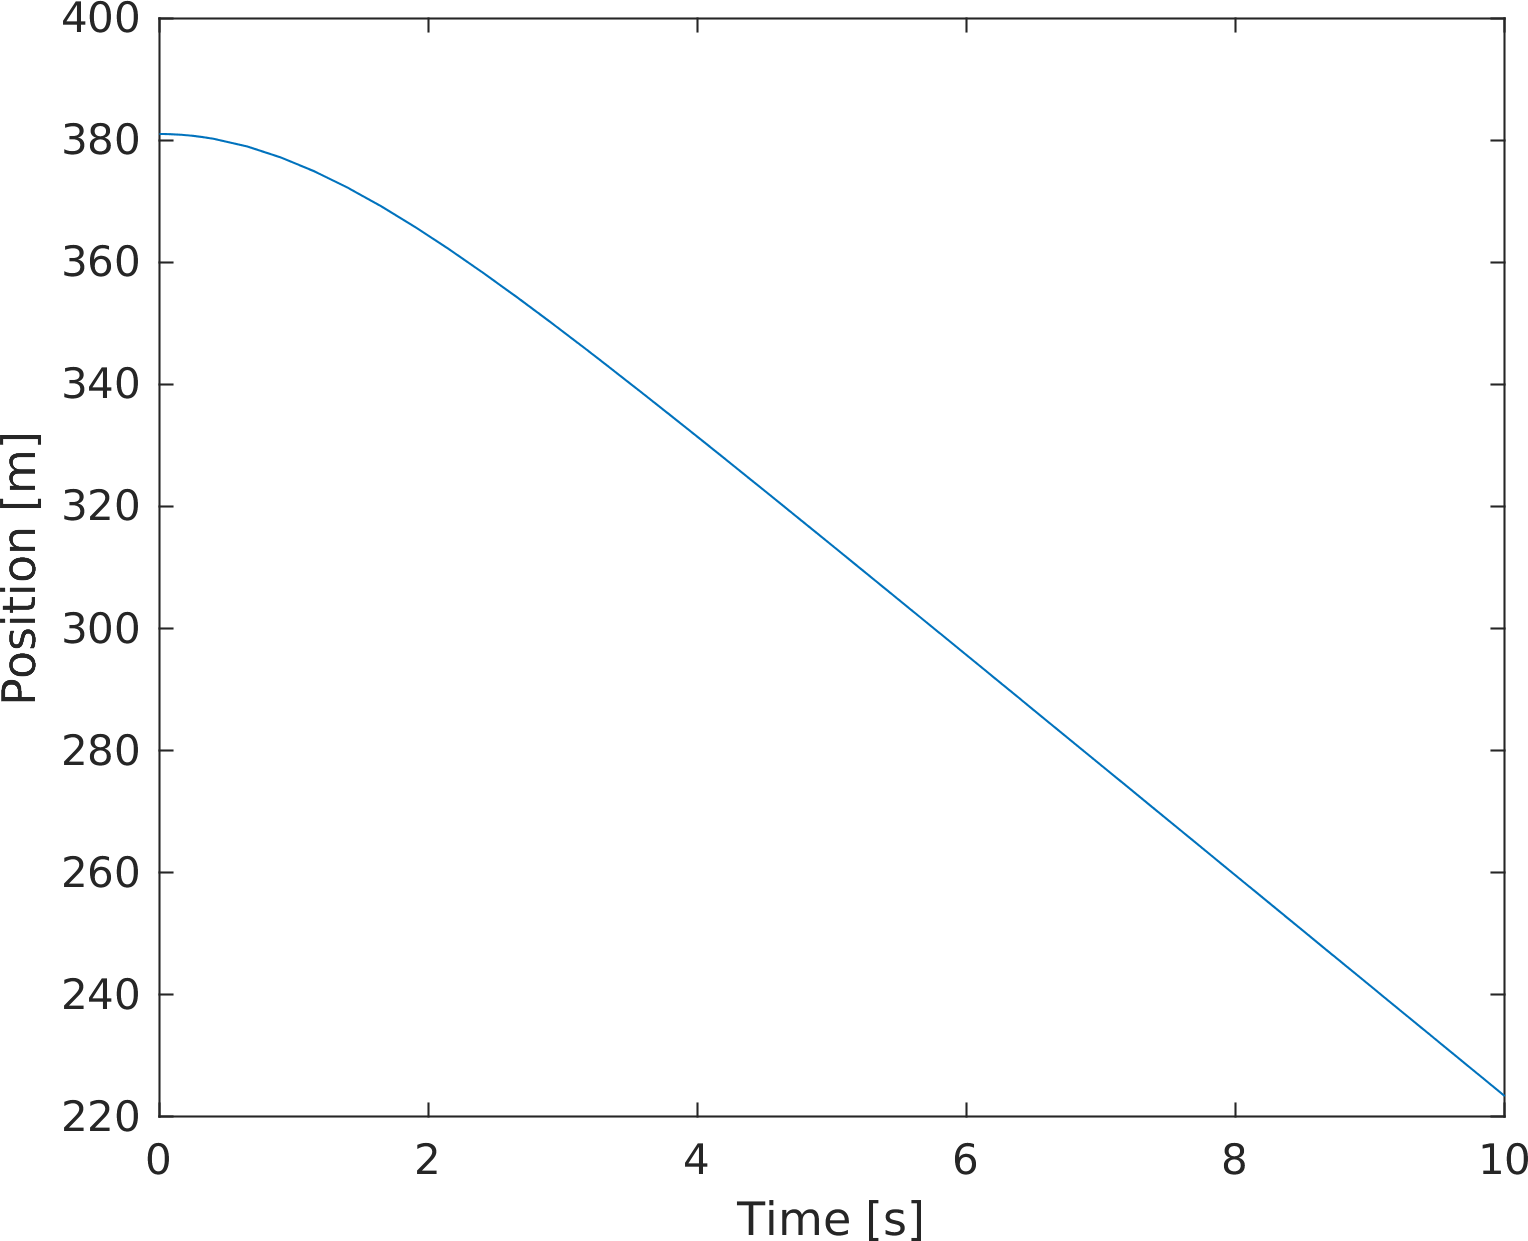
\includegraphics[width=0.7\textwidth]{w08_matrices_secondorder/lessons/penny_event_drag.png}}
\caption{Altitude versus time for a penny in free fall with air resistance}
\label{fig:penny2}
\end{figure}

Everything else is the same.  Figure~\ref{fig:penny2} shows the result.

Air resistance makes a big difference! Velocity increases until
acceleration due to drag equals acceleration due to gravity; after that, velocity is constant and position decreases linearly (and much more slowly than it would in a vacuum).

With air resistance, the time until the penny hits the sidewalk is \SI{22.4}{\second}, substantially longer than before (\SI{8.8}{\second}).

And the final velocity is \SI{18.1}{\meter \per \second}, substantially slower than before (\SI{86}{\meter \per \second}).

Here is the full script\dots
\lstinputlisting[style=mcode]{w08_matrices_secondorder/lessons/penny_event_drag.m}

\section{Chapter Review}

In this chapter, we used Newton's laws of motion to write a differential equation that describes the motion of a falling penny.

We rewrote that equation as a system of first-order differential equations, so we could use \lstinline{ode45} to solve it.  Then we ran simulations of a falling penny with and without air resistance, also known as \emph{drag}.

We defined an \emph{event} as something of interest that happens during a simulation, like a collision between moving objects, and we wrote an \emph{event function}, which allows \lstinline{ode45} to figure out when an event occurs.

In the next chapter, we extend Newtonian motion to two dimensions and model the flight of a baseball.


\section{Exercises}

Before you go on, you might want to work on the following exercise.

\begin{ex}
\index{skydiver}
\index{parachute}

In this exercise we'll model the descent of a skydiver, taking into account the change in drag when the parachute opens.

\begin{enumerate}

\item Modify the penny code from this chapter to simulate the descent of a \SI{75}{\kilogram} skydiver from an initial altitude of \SI{4000}{\meter}.
The drag constant for a skydiver without a parachute is about \SI{0.2}{\kilogram \per \meter}.
What would the velocity of the skydiver be on impact?

\item After opening their parachute, the velocity of the skydiver slows to about \SI{5}{\meter\per\second}.  Use your simulation to find the drag constant that yields a terminal velocity of \SI{5}{\meter\per\second}.

\item Increase the mass of the skydiver, and confirm that terminal velocity increases.  This phenomenon is the source of the intuition that heavy objects fall faster; in air, they do!

\item Now suppose the skydiver free falls until they get to an altitude of \SI{1000}{\meter} before opening the parachute.  How long would it take them to reach the ground?

\item What is the lowest altitude where the skydiver can open the parachute and still land at less than \SI{6}{\meter\per\second} (assuming that the parachute opens and deploys instantly)?

\end{enumerate}

% skydiver.m

\end{ex}



\begin{ex}
\label{earth}

\index{Earth}
\index{Sun}
\index{Law of Universal Gravitation}

Here's a question from the website \emph{Ask an Astronomer} (see \url{https://greenteapress.com/matlab/astro}):

\begin{quote}
If the Earth suddenly stopped orbiting the Sun, I know eventually it would be pulled in by the Sun's gravity and hit it. How long would it take the Earth to hit the Sun? I imagine it would go slowly at first and then pick up speed.
\end{quote}

Use \lstinline{ode45} to answer this question.  Here are some suggestions about how to proceed:

\begin{enumerate}

\item Look up the Law of Universal Gravitation and any constants you need. I suggest you work entirely in SI units: meters, kilograms, and newtons.

\item When the distance between the Earth and the Sun gets small, this system behaves badly, so you should use an event function to stop when the surface of the Earth reaches the surface of the Sun.

\item Express your answer in days, and plot the results as millions of kilometers versus days.

\end{enumerate}

% earth.m

\end{ex}

\chapter{Reinforcement Learning}

In this chapter, we'll introduce some of the basic concepts of \emph{reinforcement learning} as a primer for implementing a computational example.  Overall, we want to implement a learn-by-doing approach to be able to discover concepts and skills involved in applying machine learning through exploring their implementation; this brief overview provides the basics to start that exploration.

\begin{quote}
Reinforcement learning is learning what to do---how to map situations to actions---so
as to maximize a numerical reward signal. The learner is not told which actions to
take, but instead must discover which actions yield the most reward by trying them. In
the most interesting and challenging cases, actions may affect not only the immediate
reward but also the next situation and, through that, all subsequent rewards. These two
characteristics—trial-and-error search and delayed reward—are the two most important
distinguishing features of reinforcement learning.
\end{quote}
\href{http://www.incompleteideas.net/book/the-book.html}{R. Sutton and A. Barto, “Reinforcement Learning: An Introduction” 2020.}

\chapter{Reinforcement Learning: Blackjack}
\label{rl_blackjack}

\verify{Chapter content TBD. This chapter will cover Q-learning,
policy evaluation, and the \texttt{matlab\_gymnasium} blackjack
environment used in Week 11.}

\section{Q-Learning Overview}

\verify{TBD}

\section{The Blackjack Environment}

\verify{TBD --- references the \texttt{matlab\_gymnasium} repository at
\url{https://github.com/bsb808/matlab_gymnasium}.}

\section{Exercise 2: Define Your Own RL Problem}

\verify{TBD --- assignment description for student-defined RL problem.}


\backmatter
\printindex

\end{document}
